% =====================================================================
% MLLB-DL report of Maria Martinez Garcia-Taheno (experimental design,
% PyTorch, training, evaluation, reproducibility).
% Compile from report/:  pdflatex maria_mllb && bibtex maria_mllb && pdflatex x2
% Shared parts: common/ (preamble, floats, code excerpts, contributions); text: maria/.
% =====================================================================
\documentclass[11pt]{article}
% =====================================================================
% Shared preamble of the four DL reports (PRDL-DL and MLLB-DL of each author).
% Written once; each main file (report/<author>_<course>.tex) does
%     \documentclass[11pt]{article}
%     % =====================================================================
% Shared preamble of the four DL reports (PRDL-DL and MLLB-DL of each author).
% Written once; each main file (report/<author>_<course>.tex) does
%     \documentclass[11pt]{article}
%     % =====================================================================
% Shared preamble of the four DL reports (PRDL-DL and MLLB-DL of each author).
% Written once; each main file (report/<author>_<course>.tex) does
%     \documentclass[11pt]{article}
%     \input{common/preamble}
% and is compiled from the folder report/, so every path below is relative
% to report/ (also on Overleaf: upload report/ and choose the main file).
% Style taken from the ML reports (contexto_DL/ML_ref_*_main.tex.txt).
% =====================================================================

% ---------- Packages ----------
\usepackage[a4paper,margin=2.5cm]{geometry}
\usepackage[utf8]{inputenc}
\usepackage[T1]{fontenc}
\usepackage{lmodern}
\usepackage{amsmath,amssymb}
\usepackage{graphicx}
\usepackage{xcolor}
\usepackage{tabularx}
\usepackage{booktabs}
\usepackage{enumitem}
\usepackage[explicit]{titlesec}
\usepackage{fancyhdr}
\usepackage{caption}
\usepackage{float}
\usepackage{array}
\usepackage{adjustbox}   % tables shrink to the text width only when wider
\usepackage{listings}
\usepackage{siunitx}
\usepackage{cite}
\usepackage{hyperref}
\hypersetup{hidelinks}

% ---------- Colours ----------
\definecolor{etsitorange}{RGB}{237,125,49}
\definecolor{etsitblue}{RGB}{31,73,125}
\definecolor{codebg}{RGB}{245,245,245}

% ---------- Code listings (MLLB) ----------
\lstset{
  language=Python,
  backgroundcolor=\color{codebg},
  basicstyle=\ttfamily\footnotesize,
  breaklines=true,
  frame=single,
  columns=fullflexible,
  keepspaces=true,
  numbers=left,
  numberstyle=\tiny\color{gray},
  keywordstyle=\color{etsitblue}\bfseries,
  commentstyle=\color{gray}\itshape,
  showstringspaces=false
}

% ---------- Section banners (orange bar, as in the course template) ----------
\titleformat{\section}
  {\bfseries\Large\color{white}}
  {}{0pt}
  {\colorbox{etsitorange}{\parbox{\dimexpr\textwidth-4\fboxsep-12pt\relax}{\centering\thesection.\ #1}}}
\titlespacing*{\section}{0pt}{18pt}{12pt}
\titleformat{name=\section,numberless}
  {\bfseries\Large\color{white}}
  {}{0pt}
  {\colorbox{etsitorange}{\parbox{\dimexpr\textwidth-4\fboxsep-12pt\relax}{\centering#1}}}
\titlespacing*{name=\section,numberless}{0pt}{18pt}{12pt}
\titleformat{\subsection}{\bfseries\large}{\thesubsection.}{0.5em}{#1}
\titlespacing*{\subsection}{0pt}{12pt}{6pt}
\titleformat{\subsubsection}{\bfseries\normalsize}{\thesubsubsection}{0.5em}{#1}
\titlespacing*{\subsubsection}{0pt}{10pt}{4pt}

% Appendix banner (no number)
\newcommand{\appendixbanner}[1]{%
  \colorbox{etsitorange}{\parbox{\dimexpr\textwidth-4\fboxsep-12pt\relax}{\centering\bfseries\Large\color{white} #1}}%
  \vspace{12pt}}

\renewcommand{\contentsname}{CONTENTS}
\renewcommand{\listtablename}{LIST OF TABLES}
\renewcommand{\listfigurename}{LIST OF FIGURES}

\pagestyle{fancy}
\fancyhf{}
\renewcommand{\headrulewidth}{0pt}
\fancyfoot[C]{\thepage}

\captionsetup{font=small,labelfont=bf}
\graphicspath{{figures/}}
\setlength{\emergencystretch}{2em}

% ---------- Numbers ----------
% Every measured number is a macro generated from results/logs/*.json by
% report/make_numbers.py; published results come from report/published.json.
\input{numbers}

% A claim without a checked quote would be tagged with this macro; the final
% version must contain none (checked before delivery).
\newcommand{\todoverify}[1]{\textcolor{red}{\,\textsf{\footnotesize[verify: #1]}}}

% ---------- Helpers ----------
% Rounded display of a number macro (only for macros without a thousands
% separator), e.g. \intval{\edaAgeMedianNORM} -> 54; the value still comes from the log.
\newcommand{\intval}[1]{\num[round-mode=places,round-precision=0]{#1}}
\newcommand{\onedec}[1]{\num[round-mode=places,round-precision=1]{#1}}
% File or code name in typewriter font (url's \path breaks long names at / . _)
\newcommand{\file}[1]{\path{#1}}
% Report kind: \prdltrue in PRDL mains, \prdlfalse in MLLB mains
\newif\ifprdl

% Cover page: \reportcover{course}{report title}{author}{date}
\newcommand{\reportcover}[4]{%
\begin{titlepage}
\centering
\vspace*{1cm}
\IfFileExists{figures/etsit_logo.jpeg}{
\includegraphics[width=0.4\textwidth]{figures/etsit_logo.jpeg}\par}{}
\vspace{1.5cm}
{\color{etsitblue}\bfseries\Large Course:}\par
\vspace{0.5cm}
{\bfseries\huge #1}\par
\vspace{1cm}
{\Large Deep Learning Report}\par
{\bfseries\Large #2}\par
\vspace{0.5cm}
\rule{0.7\textwidth}{0.4pt}\par
\vspace{0.5cm}
{\large Master in Signal Theory and Communications (MUTSC), ETSIT -- Universidad Polit\'ecnica de Madrid}\par
\vspace{2.5cm}
\large Name: \underline{\hspace{2mm}#3\hspace{2mm}}\par
\vspace{0.3cm}
\large Team: Oriana Andrea Ferraz De Jesus and Mar\'ia Mart\'inez Garc\'ia-Tahe\~no\par
\vspace{0.5cm}
\hfill Date: \underline{\hspace{2mm}#4\hspace{2mm}}\par
\vfill
{\small Code and results: \url{https://github.com/orianafe16/ptbxl-DL}}\par
\end{titlepage}}

% and is compiled from the folder report/, so every path below is relative
% to report/ (also on Overleaf: upload report/ and choose the main file).
% Style taken from the ML reports (contexto_DL/ML_ref_*_main.tex.txt).
% =====================================================================

% ---------- Packages ----------
\usepackage[a4paper,margin=2.5cm]{geometry}
\usepackage[utf8]{inputenc}
\usepackage[T1]{fontenc}
\usepackage{lmodern}
\usepackage{amsmath,amssymb}
\usepackage{graphicx}
\usepackage{xcolor}
\usepackage{tabularx}
\usepackage{booktabs}
\usepackage{enumitem}
\usepackage[explicit]{titlesec}
\usepackage{fancyhdr}
\usepackage{caption}
\usepackage{float}
\usepackage{array}
\usepackage{adjustbox}   % tables shrink to the text width only when wider
\usepackage{listings}
\usepackage{siunitx}
\usepackage{cite}
\usepackage{hyperref}
\hypersetup{hidelinks}

% ---------- Colours ----------
\definecolor{etsitorange}{RGB}{237,125,49}
\definecolor{etsitblue}{RGB}{31,73,125}
\definecolor{codebg}{RGB}{245,245,245}

% ---------- Code listings (MLLB) ----------
\lstset{
  language=Python,
  backgroundcolor=\color{codebg},
  basicstyle=\ttfamily\footnotesize,
  breaklines=true,
  frame=single,
  columns=fullflexible,
  keepspaces=true,
  numbers=left,
  numberstyle=\tiny\color{gray},
  keywordstyle=\color{etsitblue}\bfseries,
  commentstyle=\color{gray}\itshape,
  showstringspaces=false
}

% ---------- Section banners (orange bar, as in the course template) ----------
\titleformat{\section}
  {\bfseries\Large\color{white}}
  {}{0pt}
  {\colorbox{etsitorange}{\parbox{\dimexpr\textwidth-4\fboxsep-12pt\relax}{\centering\thesection.\ #1}}}
\titlespacing*{\section}{0pt}{18pt}{12pt}
\titleformat{name=\section,numberless}
  {\bfseries\Large\color{white}}
  {}{0pt}
  {\colorbox{etsitorange}{\parbox{\dimexpr\textwidth-4\fboxsep-12pt\relax}{\centering#1}}}
\titlespacing*{name=\section,numberless}{0pt}{18pt}{12pt}
\titleformat{\subsection}{\bfseries\large}{\thesubsection.}{0.5em}{#1}
\titlespacing*{\subsection}{0pt}{12pt}{6pt}
\titleformat{\subsubsection}{\bfseries\normalsize}{\thesubsubsection}{0.5em}{#1}
\titlespacing*{\subsubsection}{0pt}{10pt}{4pt}

% Appendix banner (no number)
\newcommand{\appendixbanner}[1]{%
  \colorbox{etsitorange}{\parbox{\dimexpr\textwidth-4\fboxsep-12pt\relax}{\centering\bfseries\Large\color{white} #1}}%
  \vspace{12pt}}

\renewcommand{\contentsname}{CONTENTS}
\renewcommand{\listtablename}{LIST OF TABLES}
\renewcommand{\listfigurename}{LIST OF FIGURES}

\pagestyle{fancy}
\fancyhf{}
\renewcommand{\headrulewidth}{0pt}
\fancyfoot[C]{\thepage}

\captionsetup{font=small,labelfont=bf}
\graphicspath{{figures/}}
\setlength{\emergencystretch}{2em}

% ---------- Numbers ----------
% Every measured number is a macro generated from results/logs/*.json by
% report/make_numbers.py; published results come from report/published.json.
% numbers.tex: generated by report/make_numbers.py on 2026-11-20 19:44. Do not edit by hand.
% Sources:
%   eda: results/logs/eda.json (created 2026-11-20T17:53:34, git 8441284)
%   trivial: results/logs/trivial_e2e_s42_20261120-183809.json (created 2026-11-20T18:39:15, git f090231, uncommitted changes)
%   dense: results/logs/dense_summary.json (created 2026-11-20T19:44:51, git fcc3c3b, uncommitted changes)

% ---- eda: eda
% eda: n_records_all
\newcommand{\edaNRecordsAll}{21{,}799}
% eda: n_patients_all
\newcommand{\edaNPatientsAll}{18{,}869}
% eda: n_labelled_all
\newcommand{\edaNLabelledAll}{21{,}388}
% eda: n_records_train
\newcommand{\edaNRecordsTrain}{17{,}418}
% eda: n_patients_train
\newcommand{\edaNPatientsTrain}{15{,}023}
% eda: n_labelled_train
\newcommand{\edaNLabelledTrain}{17{,}084}
% eda: n_records_val
\newcommand{\edaNRecordsVal}{2{,}183}
% eda: n_patients_val
\newcommand{\edaNPatientsVal}{1{,}942}
% eda: n_labelled_val
\newcommand{\edaNLabelledVal}{2{,}146}
% eda: n_records_test
\newcommand{\edaNRecordsTest}{2{,}198}
% eda: n_patients_test
\newcommand{\edaNPatientsTest}{1{,}904}
% eda: n_labelled_test
\newcommand{\edaNLabelledTest}{2{,}158}
% eda: n_nosuper_all
\newcommand{\edaNNosuperAll}{411}
% eda: n_nosuper_pacemaker_field
\newcommand{\edaNNosuperPacemakerField}{277}
% eda: n_nosuper_with_rhythm_code
\newcommand{\edaNNosuperWithRhythmCode}{409}
% eda: n_nosuper_with_form_code
\newcommand{\edaNNosuperWithFormCode}{41}
% eda: n_nosuper_rhythm_only
\newcommand{\edaNNosuperRhythmOnly}{370}
% eda: n_nosuper_train
\newcommand{\edaNNosuperTrain}{334}
% eda: n_nosuper_val
\newcommand{\edaNNosuperVal}{37}
% eda: n_nosuper_test
\newcommand{\edaNNosuperTest}{40}
% eda: count_all_NORM
\newcommand{\edaCountAllNORM}{9{,}514}
% eda: prev_all_NORM
\newcommand{\edaPrevAllNORM}{0.445}
% eda: prev_all_NORM
\newcommand{\edaPrevAllNORMPct}{44.5\%}
% eda: count_all_MI
\newcommand{\edaCountAllMI}{5{,}469}
% eda: prev_all_MI
\newcommand{\edaPrevAllMI}{0.256}
% eda: prev_all_MI
\newcommand{\edaPrevAllMIPct}{25.6\%}
% eda: count_all_STTC
\newcommand{\edaCountAllSTTC}{5{,}235}
% eda: prev_all_STTC
\newcommand{\edaPrevAllSTTC}{0.245}
% eda: prev_all_STTC
\newcommand{\edaPrevAllSTTCPct}{24.5\%}
% eda: count_all_CD
\newcommand{\edaCountAllCD}{4{,}898}
% eda: prev_all_CD
\newcommand{\edaPrevAllCD}{0.229}
% eda: prev_all_CD
\newcommand{\edaPrevAllCDPct}{22.9\%}
% eda: count_all_HYP
\newcommand{\edaCountAllHYP}{2{,}649}
% eda: prev_all_HYP
\newcommand{\edaPrevAllHYP}{0.124}
% eda: prev_all_HYP
\newcommand{\edaPrevAllHYPPct}{12.4\%}
% eda: count_train_NORM
\newcommand{\edaCountTrainNORM}{7{,}596}
% eda: prev_train_NORM
\newcommand{\edaPrevTrainNORM}{0.445}
% eda: prev_train_NORM
\newcommand{\edaPrevTrainNORMPct}{44.5\%}
% eda: count_train_MI
\newcommand{\edaCountTrainMI}{4{,}379}
% eda: prev_train_MI
\newcommand{\edaPrevTrainMI}{0.256}
% eda: prev_train_MI
\newcommand{\edaPrevTrainMIPct}{25.6\%}
% eda: count_train_STTC
\newcommand{\edaCountTrainSTTC}{4{,}186}
% eda: prev_train_STTC
\newcommand{\edaPrevTrainSTTC}{0.245}
% eda: prev_train_STTC
\newcommand{\edaPrevTrainSTTCPct}{24.5\%}
% eda: count_train_CD
\newcommand{\edaCountTrainCD}{3{,}907}
% eda: prev_train_CD
\newcommand{\edaPrevTrainCD}{0.229}
% eda: prev_train_CD
\newcommand{\edaPrevTrainCDPct}{22.9\%}
% eda: count_train_HYP
\newcommand{\edaCountTrainHYP}{2{,}119}
% eda: prev_train_HYP
\newcommand{\edaPrevTrainHYP}{0.124}
% eda: prev_train_HYP
\newcommand{\edaPrevTrainHYPPct}{12.4\%}
% eda: count_val_NORM
\newcommand{\edaCountValNORM}{955}
% eda: prev_val_NORM
\newcommand{\edaPrevValNORM}{0.445}
% eda: prev_val_NORM
\newcommand{\edaPrevValNORMPct}{44.5\%}
% eda: count_val_MI
\newcommand{\edaCountValMI}{540}
% eda: prev_val_MI
\newcommand{\edaPrevValMI}{0.252}
% eda: prev_val_MI
\newcommand{\edaPrevValMIPct}{25.2\%}
% eda: count_val_STTC
\newcommand{\edaCountValSTTC}{528}
% eda: prev_val_STTC
\newcommand{\edaPrevValSTTC}{0.246}
% eda: prev_val_STTC
\newcommand{\edaPrevValSTTCPct}{24.6\%}
% eda: count_val_CD
\newcommand{\edaCountValCD}{495}
% eda: prev_val_CD
\newcommand{\edaPrevValCD}{0.231}
% eda: prev_val_CD
\newcommand{\edaPrevValCDPct}{23.1\%}
% eda: count_val_HYP
\newcommand{\edaCountValHYP}{268}
% eda: prev_val_HYP
\newcommand{\edaPrevValHYP}{0.125}
% eda: prev_val_HYP
\newcommand{\edaPrevValHYPPct}{12.5\%}
% eda: count_test_NORM
\newcommand{\edaCountTestNORM}{963}
% eda: prev_test_NORM
\newcommand{\edaPrevTestNORM}{0.446}
% eda: prev_test_NORM
\newcommand{\edaPrevTestNORMPct}{44.6\%}
% eda: count_test_MI
\newcommand{\edaCountTestMI}{550}
% eda: prev_test_MI
\newcommand{\edaPrevTestMI}{0.255}
% eda: prev_test_MI
\newcommand{\edaPrevTestMIPct}{25.5\%}
% eda: count_test_STTC
\newcommand{\edaCountTestSTTC}{521}
% eda: prev_test_STTC
\newcommand{\edaPrevTestSTTC}{0.241}
% eda: prev_test_STTC
\newcommand{\edaPrevTestSTTCPct}{24.1\%}
% eda: count_test_CD
\newcommand{\edaCountTestCD}{496}
% eda: prev_test_CD
\newcommand{\edaPrevTestCD}{0.230}
% eda: prev_test_CD
\newcommand{\edaPrevTestCDPct}{23.0\%}
% eda: count_test_HYP
\newcommand{\edaCountTestHYP}{262}
% eda: prev_test_HYP
\newcommand{\edaPrevTestHYP}{0.121}
% eda: prev_test_HYP
\newcommand{\edaPrevTestHYPPct}{12.1\%}
% eda: imbalance_ratio_train
\newcommand{\edaImbalanceRatioTrain}{3.585}
% eda: n_with_1_labels
\newcommand{\edaNWithOneLabels}{16{,}244}
% eda: n_with_2_labels
\newcommand{\edaNWithTwoLabels}{4{,}068}
% eda: n_with_3_labels
\newcommand{\edaNWithThreeLabels}{919}
% eda: n_with_4_labels
\newcommand{\edaNWithFourLabels}{157}
% eda: frac_multilabel_all
\newcommand{\edaFracMultilabelAll}{0.241}
% eda: frac_multilabel_all
\newcommand{\edaFracMultilabelAllPct}{24.1\%}
% eda: n_norm_with_other
\newcommand{\edaNNormWithOther}{445}
% eda: n_combinations
\newcommand{\edaNCombinations}{22}
% eda: max_fold_prev_gap_pp
\newcommand{\edaMaxFoldPrevGapPp}{1.610}
% eda: n_age_over89_all
\newcommand{\edaNAgeOverEightNineAll}{293}
% eda: n_age_missing_all
\newcommand{\edaNAgeMissingAll}{0}
% eda: age_min_all
\newcommand{\edaAgeMinAll}{2.000}
% eda: age_max_all
\newcommand{\edaAgeMaxAll}{89.000}
% eda: age_median_all
\newcommand{\edaAgeMedianAll}{61.000}
% eda: age_q1_all
\newcommand{\edaAgeQOneAll}{50.000}
% eda: age_q3_all
\newcommand{\edaAgeQThreeAll}{72.000}
% eda: n_sex0_all
\newcommand{\edaNSexZeroAll}{11{,}354}
% eda: n_sex1_all
\newcommand{\edaNSexOneAll}{10{,}445}
% eda: frac_sex1_all
\newcommand{\edaFracSexOneAll}{0.479}
% eda: frac_sex1_all
\newcommand{\edaFracSexOneAllPct}{47.9\%}
% eda: age_median_train
\newcommand{\edaAgeMedianTrain}{61.000}
% eda: age_q1_train
\newcommand{\edaAgeQOneTrain}{50.000}
% eda: age_q3_train
\newcommand{\edaAgeQThreeTrain}{72.000}
% eda: n_sex0_train
\newcommand{\edaNSexZeroTrain}{9{,}089}
% eda: n_sex1_train
\newcommand{\edaNSexOneTrain}{8{,}329}
% eda: frac_sex1_train
\newcommand{\edaFracSexOneTrain}{0.478}
% eda: frac_sex1_train
\newcommand{\edaFracSexOneTrainPct}{47.8\%}
% eda: age_median_val
\newcommand{\edaAgeMedianVal}{62.000}
% eda: age_q1_val
\newcommand{\edaAgeQOneVal}{49.000}
% eda: age_q3_val
\newcommand{\edaAgeQThreeVal}{73.000}
% eda: n_sex0_val
\newcommand{\edaNSexZeroVal}{1{,}133}
% eda: n_sex1_val
\newcommand{\edaNSexOneVal}{1{,}050}
% eda: frac_sex1_val
\newcommand{\edaFracSexOneVal}{0.481}
% eda: frac_sex1_val
\newcommand{\edaFracSexOneValPct}{48.1\%}
% eda: age_median_test
\newcommand{\edaAgeMedianTest}{63.000}
% eda: age_q1_test
\newcommand{\edaAgeQOneTest}{50.000}
% eda: age_q3_test
\newcommand{\edaAgeQThreeTest}{74.000}
% eda: n_sex0_test
\newcommand{\edaNSexZeroTest}{1{,}132}
% eda: n_sex1_test
\newcommand{\edaNSexOneTest}{1{,}066}
% eda: frac_sex1_test
\newcommand{\edaFracSexOneTest}{0.485}
% eda: frac_sex1_test
\newcommand{\edaFracSexOneTestPct}{48.5\%}
% eda: age_median_NORM
\newcommand{\edaAgeMedianNORM}{54.000}
% eda: frac_sex1_NORM
\newcommand{\edaFracSexOneNORM}{0.539}
% eda: frac_sex1_NORM
\newcommand{\edaFracSexOneNORMPct}{53.9\%}
% eda: age_median_MI
\newcommand{\edaAgeMedianMI}{67.000}
% eda: frac_sex1_MI
\newcommand{\edaFracSexOneMI}{0.377}
% eda: frac_sex1_MI
\newcommand{\edaFracSexOneMIPct}{37.7\%}
% eda: age_median_STTC
\newcommand{\edaAgeMedianSTTC}{67.000}
% eda: frac_sex1_STTC
\newcommand{\edaFracSexOneSTTC}{0.510}
% eda: frac_sex1_STTC
\newcommand{\edaFracSexOneSTTCPct}{51.0\%}
% eda: age_median_CD
\newcommand{\edaAgeMedianCD}{67.000}
% eda: frac_sex1_CD
\newcommand{\edaFracSexOneCD}{0.388}
% eda: frac_sex1_CD
\newcommand{\edaFracSexOneCDPct}{38.8\%}
% eda: age_median_HYP
\newcommand{\edaAgeMedianHYP}{67.000}
% eda: frac_sex1_HYP
\newcommand{\edaFracSexOneHYP}{0.426}
% eda: frac_sex1_HYP
\newcommand{\edaFracSexOneHYPPct}{42.6\%}
% eda: n_height_missing_all
\newcommand{\edaNHeightMissingAll}{14{,}825}
% eda: n_weight_missing_all
\newcommand{\edaNWeightMissingAll}{12{,}378}
% eda: n_patients_one_record
\newcommand{\edaNPatientsOneRecord}{16{,}758}
% eda: n_patients_several_records
\newcommand{\edaNPatientsSeveralRecords}{2{,}111}
% eda: max_records_per_patient
\newcommand{\edaMaxRecordsPerPatient}{10}
% eda: n_baseline_drift_all
\newcommand{\edaNBaselineDriftAll}{1{,}598}
% eda: n_static_noise_all
\newcommand{\edaNStaticNoiseAll}{3{,}260}
% eda: n_burst_noise_all
\newcommand{\edaNBurstNoiseAll}{612}
% eda: n_electrodes_problems_all
\newcommand{\edaNElectrodesProblemsAll}{30}
% eda: n_extra_beats_all
\newcommand{\edaNExtraBeatsAll}{1{,}949}
% eda: n_pacemaker_all
\newcommand{\edaNPacemakerAll}{291}
% eda: n_any_quality_flag_all
\newcommand{\edaNAnyQualityFlagAll}{6{,}610}
% eda: frac_any_quality_flag_all
\newcommand{\edaFracAnyQualityFlagAll}{0.303}
% eda: frac_any_quality_flag_all
\newcommand{\edaFracAnyQualityFlagAllPct}{30.3\%}
% eda: n_baseline_drift_train
\newcommand{\edaNBaselineDriftTrain}{1{,}133}
% eda: n_static_noise_train
\newcommand{\edaNStaticNoiseTrain}{2{,}613}
% eda: n_burst_noise_train
\newcommand{\edaNBurstNoiseTrain}{520}
% eda: n_electrodes_problems_train
\newcommand{\edaNElectrodesProblemsTrain}{23}
% eda: n_extra_beats_train
\newcommand{\edaNExtraBeatsTrain}{1{,}557}
% eda: n_pacemaker_train
\newcommand{\edaNPacemakerTrain}{234}
% eda: n_any_quality_flag_train
\newcommand{\edaNAnyQualityFlagTrain}{5{,}232}
% eda: frac_any_quality_flag_train
\newcommand{\edaFracAnyQualityFlagTrain}{0.300}
% eda: frac_any_quality_flag_train
\newcommand{\edaFracAnyQualityFlagTrainPct}{30.0\%}
% eda: n_baseline_drift_val
\newcommand{\edaNBaselineDriftVal}{229}
% eda: n_static_noise_val
\newcommand{\edaNStaticNoiseVal}{331}
% eda: n_burst_noise_val
\newcommand{\edaNBurstNoiseVal}{52}
% eda: n_electrodes_problems_val
\newcommand{\edaNElectrodesProblemsVal}{4}
% eda: n_extra_beats_val
\newcommand{\edaNExtraBeatsVal}{194}
% eda: n_pacemaker_val
\newcommand{\edaNPacemakerVal}{28}
% eda: n_any_quality_flag_val
\newcommand{\edaNAnyQualityFlagVal}{699}
% eda: frac_any_quality_flag_val
\newcommand{\edaFracAnyQualityFlagVal}{0.320}
% eda: frac_any_quality_flag_val
\newcommand{\edaFracAnyQualityFlagValPct}{32.0\%}
% eda: n_baseline_drift_test
\newcommand{\edaNBaselineDriftTest}{236}
% eda: n_static_noise_test
\newcommand{\edaNStaticNoiseTest}{316}
% eda: n_burst_noise_test
\newcommand{\edaNBurstNoiseTest}{40}
% eda: n_electrodes_problems_test
\newcommand{\edaNElectrodesProblemsTest}{3}
% eda: n_extra_beats_test
\newcommand{\edaNExtraBeatsTest}{198}
% eda: n_pacemaker_test
\newcommand{\edaNPacemakerTest}{29}
% eda: n_any_quality_flag_test
\newcommand{\edaNAnyQualityFlagTest}{679}
% eda: frac_any_quality_flag_test
\newcommand{\edaFracAnyQualityFlagTest}{0.309}
% eda: frac_any_quality_flag_test
\newcommand{\edaFracAnyQualityFlagTestPct}{30.9\%}
% eda: n_validated_by_human_all
\newcommand{\edaNValidatedByHumanAll}{16{,}056}
% eda: frac_validated_by_human_all
\newcommand{\edaFracValidatedByHumanAll}{0.737}
% eda: frac_validated_by_human_all
\newcommand{\edaFracValidatedByHumanAllPct}{73.7\%}
% eda: n_validated_by_human_train
\newcommand{\edaNValidatedByHumanTrain}{11{,}675}
% eda: frac_validated_by_human_train
\newcommand{\edaFracValidatedByHumanTrain}{0.670}
% eda: frac_validated_by_human_train
\newcommand{\edaFracValidatedByHumanTrainPct}{67.0\%}
% eda: n_validated_by_human_val
\newcommand{\edaNValidatedByHumanVal}{2{,}183}
% eda: frac_validated_by_human_val
\newcommand{\edaFracValidatedByHumanVal}{1.000}
% eda: frac_validated_by_human_val
\newcommand{\edaFracValidatedByHumanValPct}{100.0\%}
% eda: n_validated_by_human_test
\newcommand{\edaNValidatedByHumanTest}{2{,}198}
% eda: frac_validated_by_human_test
\newcommand{\edaFracValidatedByHumanTest}{1.000}
% eda: frac_validated_by_human_test
\newcommand{\edaFracValidatedByHumanTestPct}{100.0\%}
% eda: n_second_opinion_all
\newcommand{\edaNSecondOpinionAll}{555}
% eda: n_signal_records_train
\newcommand{\edaNSignalRecordsTrain}{17{,}084}
% eda: lead_mean_I
\newcommand{\edaLeadMeanI}{\ensuremath{-}0.002}
% eda: lead_std_I
\newcommand{\edaLeadStdI}{0.160}
% eda: lead_ptp_median_I
\newcommand{\edaLeadPtpMedianI}{1.039}
% eda: lead_mean_II
\newcommand{\edaLeadMeanII}{\ensuremath{-}0.002}
% eda: lead_std_II
\newcommand{\edaLeadStdII}{0.159}
% eda: lead_ptp_median_II
\newcommand{\edaLeadPtpMedianII}{1.041}
% eda: lead_mean_III
\newcommand{\edaLeadMeanIII}{0.000}
% eda: lead_std_III
\newcommand{\edaLeadStdIII}{0.160}
% eda: lead_ptp_median_III
\newcommand{\edaLeadPtpMedianIII}{0.888}
% eda: lead_mean_AVR
\newcommand{\edaLeadMeanAVR}{0.002}
% eda: lead_std_AVR
\newcommand{\edaLeadStdAVR}{0.138}
% eda: lead_ptp_median_AVR
\newcommand{\edaLeadPtpMedianAVR}{0.949}
% eda: lead_mean_AVL
\newcommand{\edaLeadMeanAVL}{\ensuremath{-}0.001}
% eda: lead_std_AVL
\newcommand{\edaLeadStdAVL}{0.139}
% eda: lead_ptp_median_AVL
\newcommand{\edaLeadPtpMedianAVL}{0.821}
% eda: lead_mean_AVF
\newcommand{\edaLeadMeanAVF}{\ensuremath{-}0.001}
% eda: lead_std_AVF
\newcommand{\edaLeadStdAVF}{0.138}
% eda: lead_ptp_median_AVF
\newcommand{\edaLeadPtpMedianAVF}{0.811}
% eda: lead_mean_V1
\newcommand{\edaLeadMeanVOne}{0.000}
% eda: lead_std_V1
\newcommand{\edaLeadStdVOne}{0.234}
% eda: lead_ptp_median_V1
\newcommand{\edaLeadPtpMedianVOne}{1.246}
% eda: lead_mean_V2
\newcommand{\edaLeadMeanVTwo}{\ensuremath{-}0.001}
% eda: lead_std_V2
\newcommand{\edaLeadStdVTwo}{0.334}
% eda: lead_ptp_median_V2
\newcommand{\edaLeadPtpMedianVTwo}{1.962}
% eda: lead_mean_V3
\newcommand{\edaLeadMeanVThree}{\ensuremath{-}0.002}
% eda: lead_std_V3
\newcommand{\edaLeadStdVThree}{0.328}
% eda: lead_ptp_median_V3
\newcommand{\edaLeadPtpMedianVThree}{2.016}
% eda: lead_mean_V4
\newcommand{\edaLeadMeanVFour}{\ensuremath{-}0.001}
% eda: lead_std_V4
\newcommand{\edaLeadStdVFour}{0.293}
% eda: lead_ptp_median_V4
\newcommand{\edaLeadPtpMedianVFour}{2.106}
% eda: lead_mean_V5
\newcommand{\edaLeadMeanVFive}{\ensuremath{-}0.001}
% eda: lead_std_V5
\newcommand{\edaLeadStdVFive}{0.272}
% eda: lead_ptp_median_V5
\newcommand{\edaLeadPtpMedianVFive}{1.815}
% eda: lead_mean_V6
\newcommand{\edaLeadMeanVSix}{\ensuremath{-}0.002}
% eda: lead_std_V6
\newcommand{\edaLeadStdVSix}{0.281}
% eda: lead_ptp_median_V6
\newcommand{\edaLeadPtpMedianVSix}{1.385}
% eda: n_nan_values_train
\newcommand{\edaNNanValuesTrain}{0}
% eda: n_flat_leads_train
\newcommand{\edaNFlatLeadsTrain}{1}
% eda: lead_std_ratio_max_min
\newcommand{\edaLeadStdRatioMaxMin}{2.422}

% ---- trivial: trivial_e2e_s42_20261120-183809
% trivial: best_epoch
\newcommand{\trivialBestEpoch}{28}
% trivial: epochs_run
\newcommand{\trivialEpochsRun}{33}
% trivial: n_params
\newcommand{\trivialNParams}{125}
% trivial: n_trainable
\newcommand{\trivialNTrainable}{125}
% trivial: train_time_s
\newcommand{\trivialTrainTimeS}{37.655}
% trivial: threshold_NORM
\newcommand{\trivialThresholdNORM}{0.360}
% trivial: threshold_MI
\newcommand{\trivialThresholdMI}{0.250}
% trivial: threshold_STTC
\newcommand{\trivialThresholdSTTC}{0.240}
% trivial: threshold_CD
\newcommand{\trivialThresholdCD}{0.240}
% trivial: threshold_HYP
\newcommand{\trivialThresholdHYP}{0.150}
% trivial: val_loss
\newcommand{\trivialValLoss}{0.490}
% trivial: val_macro_auroc
\newcommand{\trivialValMacroAuroc}{0.741}
% trivial: val_macro_auroc_lo
\newcommand{\trivialValMacroAurocLo}{0.727}
% trivial: val_macro_auroc_hi
\newcommand{\trivialValMacroAurocHi}{0.753}
% trivial: val_macro_f1
\newcommand{\trivialValMacroFOne}{0.534}
% trivial: val_macro_f1_lo
\newcommand{\trivialValMacroFOneLo}{0.517}
% trivial: val_macro_f1_hi
\newcommand{\trivialValMacroFOneHi}{0.548}
% trivial: val_auroc_NORM
\newcommand{\trivialValAurocNORM}{0.758}
% trivial: val_auroc_NORM_lo
\newcommand{\trivialValAurocNORMLo}{0.737}
% trivial: val_auroc_NORM_hi
\newcommand{\trivialValAurocNORMHi}{0.777}
% trivial: val_f1_NORM
\newcommand{\trivialValFOneNORM}{0.694}
% trivial: val_auroc_MI
\newcommand{\trivialValAurocMI}{0.729}
% trivial: val_auroc_MI_lo
\newcommand{\trivialValAurocMILo}{0.701}
% trivial: val_auroc_MI_hi
\newcommand{\trivialValAurocMIHi}{0.753}
% trivial: val_f1_MI
\newcommand{\trivialValFOneMI}{0.525}
% trivial: val_auroc_STTC
\newcommand{\trivialValAurocSTTC}{0.655}
% trivial: val_auroc_STTC_lo
\newcommand{\trivialValAurocSTTCLo}{0.625}
% trivial: val_auroc_STTC_hi
\newcommand{\trivialValAurocSTTCHi}{0.683}
% trivial: val_f1_STTC
\newcommand{\trivialValFOneSTTC}{0.455}
% trivial: val_auroc_CD
\newcommand{\trivialValAurocCD}{0.736}
% trivial: val_auroc_CD_lo
\newcommand{\trivialValAurocCDLo}{0.706}
% trivial: val_auroc_CD_hi
\newcommand{\trivialValAurocCDHi}{0.761}
% trivial: val_f1_CD
\newcommand{\trivialValFOneCD}{0.508}
% trivial: val_auroc_HYP
\newcommand{\trivialValAurocHYP}{0.829}
% trivial: val_auroc_HYP_lo
\newcommand{\trivialValAurocHYPLo}{0.802}
% trivial: val_auroc_HYP_hi
\newcommand{\trivialValAurocHYPHi}{0.853}
% trivial: val_f1_HYP
\newcommand{\trivialValFOneHYP}{0.487}
% trivial: test_loss
\newcommand{\trivialTestLoss}{0.495}
% trivial: test_macro_auroc
\newcommand{\trivialTestMacroAuroc}{0.718}
% trivial: test_macro_auroc_lo
\newcommand{\trivialTestMacroAurocLo}{0.702}
% trivial: test_macro_auroc_hi
\newcommand{\trivialTestMacroAurocHi}{0.732}
% trivial: test_macro_f1
\newcommand{\trivialTestMacroFOne}{0.503}
% trivial: test_macro_f1_lo
\newcommand{\trivialTestMacroFOneLo}{0.485}
% trivial: test_macro_f1_hi
\newcommand{\trivialTestMacroFOneHi}{0.519}
% trivial: test_auroc_NORM
\newcommand{\trivialTestAurocNORM}{0.729}
% trivial: test_auroc_NORM_lo
\newcommand{\trivialTestAurocNORMLo}{0.706}
% trivial: test_auroc_NORM_hi
\newcommand{\trivialTestAurocNORMHi}{0.751}
% trivial: test_f1_NORM
\newcommand{\trivialTestFOneNORM}{0.681}
% trivial: test_auroc_MI
\newcommand{\trivialTestAurocMI}{0.727}
% trivial: test_auroc_MI_lo
\newcommand{\trivialTestAurocMILo}{0.700}
% trivial: test_auroc_MI_hi
\newcommand{\trivialTestAurocMIHi}{0.753}
% trivial: test_f1_MI
\newcommand{\trivialTestFOneMI}{0.508}
% trivial: test_auroc_STTC
\newcommand{\trivialTestAurocSTTC}{0.626}
% trivial: test_auroc_STTC_lo
\newcommand{\trivialTestAurocSTTCLo}{0.597}
% trivial: test_auroc_STTC_hi
\newcommand{\trivialTestAurocSTTCHi}{0.656}
% trivial: test_f1_STTC
\newcommand{\trivialTestFOneSTTC}{0.415}
% trivial: test_auroc_CD
\newcommand{\trivialTestAurocCD}{0.712}
% trivial: test_auroc_CD_lo
\newcommand{\trivialTestAurocCDLo}{0.681}
% trivial: test_auroc_CD_hi
\newcommand{\trivialTestAurocCDHi}{0.743}
% trivial: test_f1_CD
\newcommand{\trivialTestFOneCD}{0.482}
% trivial: test_auroc_HYP
\newcommand{\trivialTestAurocHYP}{0.796}
% trivial: test_auroc_HYP_lo
\newcommand{\trivialTestAurocHYPLo}{0.767}
% trivial: test_auroc_HYP_hi
\newcommand{\trivialTestAurocHYPHi}{0.822}
% trivial: test_f1_HYP
\newcommand{\trivialTestFOneHYP}{0.429}

% ---- dense: dense_summary
% dense: params_base
\newcommand{\denseParamsBase}{3{,}140{,}357}
% dense: val_auroc_mean_base
\newcommand{\denseValAurocMeanBase}{0.757}
% dense: val_auroc_sd_base
\newcommand{\denseValAurocSdBase}{0.002}
% dense: best_epoch_mean_base
\newcommand{\denseBestEpochMeanBase}{17.333}
% dense: epoch_time_mean_base
\newcommand{\denseEpochTimeMeanBase}{1.362}
% dense: val_auroc_first_base
\newcommand{\denseValAurocFirstBase}{0.759}
% dense: val_auroc_lo_first_base
\newcommand{\denseValAurocLoFirstBase}{0.745}
% dense: val_auroc_hi_first_base
\newcommand{\denseValAurocHiFirstBase}{0.772}
% dense: params_no_norm
\newcommand{\denseParamsNoNorm}{3{,}140{,}357}
% dense: val_auroc_mean_no_norm
\newcommand{\denseValAurocMeanNoNorm}{0.760}
% dense: val_auroc_sd_no_norm
\newcommand{\denseValAurocSdNoNorm}{0.002}
% dense: best_epoch_mean_no_norm
\newcommand{\denseBestEpochMeanNoNorm}{19.000}
% dense: epoch_time_mean_no_norm
\newcommand{\denseEpochTimeMeanNoNorm}{1.252}
% dense: val_auroc_first_no_norm
\newcommand{\denseValAurocFirstNoNorm}{0.758}
% dense: val_auroc_lo_first_no_norm
\newcommand{\denseValAurocLoFirstNoNorm}{0.744}
% dense: val_auroc_hi_first_no_norm
\newcommand{\denseValAurocHiFirstNoNorm}{0.770}
% dense: diff_s42_no_norm
\newcommand{\denseDiffSFourTwoNoNorm}{\ensuremath{-}0.001}
% dense: diff_lo_s42_no_norm
\newcommand{\denseDiffLoSFourTwoNoNorm}{\ensuremath{-}0.009}
% dense: diff_hi_s42_no_norm
\newcommand{\denseDiffHiSFourTwoNoNorm}{0.007}
% dense: diff_s43_no_norm
\newcommand{\denseDiffSFourThreeNoNorm}{0.005}
% dense: diff_lo_s43_no_norm
\newcommand{\denseDiffLoSFourThreeNoNorm}{\ensuremath{-}0.004}
% dense: diff_hi_s43_no_norm
\newcommand{\denseDiffHiSFourThreeNoNorm}{0.014}
% dense: diff_s44_no_norm
\newcommand{\denseDiffSFourFourNoNorm}{0.004}
% dense: diff_lo_s44_no_norm
\newcommand{\denseDiffLoSFourFourNoNorm}{\ensuremath{-}0.005}
% dense: diff_hi_s44_no_norm
\newcommand{\denseDiffHiSFourFourNoNorm}{0.013}
% dense: diff_mean_no_norm
\newcommand{\denseDiffMeanNoNorm}{0.003}
% dense: n_seeds_better_no_norm
\newcommand{\denseNSeedsBetterNoNorm}{0}
% dense: n_seeds_worse_no_norm
\newcommand{\denseNSeedsWorseNoNorm}{0}
% dense: n_seeds_compared_no_norm
\newcommand{\denseNSeedsComparedNoNorm}{3}
% dense: params_no_bn
\newcommand{\denseParamsNoBn}{3{,}139{,}333}
% dense: val_auroc_mean_no_bn
\newcommand{\denseValAurocMeanNoBn}{0.704}
% dense: val_auroc_sd_no_bn
\newcommand{\denseValAurocSdNoBn}{0.003}
% dense: best_epoch_mean_no_bn
\newcommand{\denseBestEpochMeanNoBn}{12.000}
% dense: epoch_time_mean_no_bn
\newcommand{\denseEpochTimeMeanNoBn}{1.555}
% dense: val_auroc_first_no_bn
\newcommand{\denseValAurocFirstNoBn}{0.706}
% dense: val_auroc_lo_first_no_bn
\newcommand{\denseValAurocLoFirstNoBn}{0.691}
% dense: val_auroc_hi_first_no_bn
\newcommand{\denseValAurocHiFirstNoBn}{0.721}
% dense: diff_s42_no_bn
\newcommand{\denseDiffSFourTwoNoBn}{\ensuremath{-}0.052}
% dense: diff_lo_s42_no_bn
\newcommand{\denseDiffLoSFourTwoNoBn}{\ensuremath{-}0.066}
% dense: diff_hi_s42_no_bn
\newcommand{\denseDiffHiSFourTwoNoBn}{\ensuremath{-}0.039}
% dense: diff_s43_no_bn
\newcommand{\denseDiffSFourThreeNoBn}{\ensuremath{-}0.053}
% dense: diff_lo_s43_no_bn
\newcommand{\denseDiffLoSFourThreeNoBn}{\ensuremath{-}0.067}
% dense: diff_hi_s43_no_bn
\newcommand{\denseDiffHiSFourThreeNoBn}{\ensuremath{-}0.040}
% dense: diff_s44_no_bn
\newcommand{\denseDiffSFourFourNoBn}{\ensuremath{-}0.053}
% dense: diff_lo_s44_no_bn
\newcommand{\denseDiffLoSFourFourNoBn}{\ensuremath{-}0.066}
% dense: diff_hi_s44_no_bn
\newcommand{\denseDiffHiSFourFourNoBn}{\ensuremath{-}0.040}
% dense: diff_mean_no_bn
\newcommand{\denseDiffMeanNoBn}{\ensuremath{-}0.053}
% dense: n_seeds_better_no_bn
\newcommand{\denseNSeedsBetterNoBn}{0}
% dense: n_seeds_worse_no_bn
\newcommand{\denseNSeedsWorseNoBn}{3}
% dense: n_seeds_compared_no_bn
\newcommand{\denseNSeedsComparedNoBn}{3}
% dense: params_no_norm_no_bn
\newcommand{\denseParamsNoNormNoBn}{3{,}139{,}333}
% dense: val_auroc_mean_no_norm_no_bn
\newcommand{\denseValAurocMeanNoNormNoBn}{0.719}
% dense: val_auroc_sd_no_norm_no_bn
\newcommand{\denseValAurocSdNoNormNoBn}{0.005}
% dense: best_epoch_mean_no_norm_no_bn
\newcommand{\denseBestEpochMeanNoNormNoBn}{10.333}
% dense: epoch_time_mean_no_norm_no_bn
\newcommand{\denseEpochTimeMeanNoNormNoBn}{1.124}
% dense: val_auroc_first_no_norm_no_bn
\newcommand{\denseValAurocFirstNoNormNoBn}{0.713}
% dense: val_auroc_lo_first_no_norm_no_bn
\newcommand{\denseValAurocLoFirstNoNormNoBn}{0.696}
% dense: val_auroc_hi_first_no_norm_no_bn
\newcommand{\denseValAurocHiFirstNoNormNoBn}{0.728}
% dense: diff_s42_no_norm_no_bn
\newcommand{\denseDiffSFourTwoNoNormNoBn}{\ensuremath{-}0.046}
% dense: diff_lo_s42_no_norm_no_bn
\newcommand{\denseDiffLoSFourTwoNoNormNoBn}{\ensuremath{-}0.058}
% dense: diff_hi_s42_no_norm_no_bn
\newcommand{\denseDiffHiSFourTwoNoNormNoBn}{\ensuremath{-}0.034}
% dense: diff_s43_no_norm_no_bn
\newcommand{\denseDiffSFourThreeNoNormNoBn}{\ensuremath{-}0.033}
% dense: diff_lo_s43_no_norm_no_bn
\newcommand{\denseDiffLoSFourThreeNoNormNoBn}{\ensuremath{-}0.044}
% dense: diff_hi_s43_no_norm_no_bn
\newcommand{\denseDiffHiSFourThreeNoNormNoBn}{\ensuremath{-}0.022}
% dense: diff_s44_no_norm_no_bn
\newcommand{\denseDiffSFourFourNoNormNoBn}{\ensuremath{-}0.035}
% dense: diff_lo_s44_no_norm_no_bn
\newcommand{\denseDiffLoSFourFourNoNormNoBn}{\ensuremath{-}0.046}
% dense: diff_hi_s44_no_norm_no_bn
\newcommand{\denseDiffHiSFourFourNoNormNoBn}{\ensuremath{-}0.024}
% dense: diff_mean_no_norm_no_bn
\newcommand{\denseDiffMeanNoNormNoBn}{\ensuremath{-}0.038}
% dense: n_seeds_better_no_norm_no_bn
\newcommand{\denseNSeedsBetterNoNormNoBn}{0}
% dense: n_seeds_worse_no_norm_no_bn
\newcommand{\denseNSeedsWorseNoNormNoBn}{3}
% dense: n_seeds_compared_no_norm_no_bn
\newcommand{\denseNSeedsComparedNoNormNoBn}{3}
% dense: params_no_dropout
\newcommand{\denseParamsNoDropout}{3{,}140{,}357}
% dense: val_auroc_mean_no_dropout
\newcommand{\denseValAurocMeanNoDropout}{0.725}
% dense: val_auroc_sd_no_dropout
\newcommand{\denseValAurocSdNoDropout}{0.007}
% dense: best_epoch_mean_no_dropout
\newcommand{\denseBestEpochMeanNoDropout}{3.000}
% dense: epoch_time_mean_no_dropout
\newcommand{\denseEpochTimeMeanNoDropout}{1.558}
% dense: val_auroc_first_no_dropout
\newcommand{\denseValAurocFirstNoDropout}{0.720}
% dense: val_auroc_lo_first_no_dropout
\newcommand{\denseValAurocLoFirstNoDropout}{0.706}
% dense: val_auroc_hi_first_no_dropout
\newcommand{\denseValAurocHiFirstNoDropout}{0.734}
% dense: diff_s42_no_dropout
\newcommand{\denseDiffSFourTwoNoDropout}{\ensuremath{-}0.039}
% dense: diff_lo_s42_no_dropout
\newcommand{\denseDiffLoSFourTwoNoDropout}{\ensuremath{-}0.049}
% dense: diff_hi_s42_no_dropout
\newcommand{\denseDiffHiSFourTwoNoDropout}{\ensuremath{-}0.029}
% dense: diff_s43_no_dropout
\newcommand{\denseDiffSFourThreeNoDropout}{\ensuremath{-}0.022}
% dense: diff_lo_s43_no_dropout
\newcommand{\denseDiffLoSFourThreeNoDropout}{\ensuremath{-}0.033}
% dense: diff_hi_s43_no_dropout
\newcommand{\denseDiffHiSFourThreeNoDropout}{\ensuremath{-}0.011}
% dense: diff_s44_no_dropout
\newcommand{\denseDiffSFourFourNoDropout}{\ensuremath{-}0.037}
% dense: diff_lo_s44_no_dropout
\newcommand{\denseDiffLoSFourFourNoDropout}{\ensuremath{-}0.047}
% dense: diff_hi_s44_no_dropout
\newcommand{\denseDiffHiSFourFourNoDropout}{\ensuremath{-}0.026}
% dense: diff_mean_no_dropout
\newcommand{\denseDiffMeanNoDropout}{\ensuremath{-}0.032}
% dense: n_seeds_better_no_dropout
\newcommand{\denseNSeedsBetterNoDropout}{0}
% dense: n_seeds_worse_no_dropout
\newcommand{\denseNSeedsWorseNoDropout}{3}
% dense: n_seeds_compared_no_dropout
\newcommand{\denseNSeedsComparedNoDropout}{3}
% dense: params_dropout02
\newcommand{\denseParamsDropoutZeroTwo}{3{,}140{,}357}
% dense: val_auroc_mean_dropout02
\newcommand{\denseValAurocMeanDropoutZeroTwo}{0.738}
% dense: val_auroc_sd_dropout02
\newcommand{\denseValAurocSdDropoutZeroTwo}{0.001}
% dense: best_epoch_mean_dropout02
\newcommand{\denseBestEpochMeanDropoutZeroTwo}{5.333}
% dense: epoch_time_mean_dropout02
\newcommand{\denseEpochTimeMeanDropoutZeroTwo}{1.605}
% dense: val_auroc_first_dropout02
\newcommand{\denseValAurocFirstDropoutZeroTwo}{0.739}
% dense: val_auroc_lo_first_dropout02
\newcommand{\denseValAurocLoFirstDropoutZeroTwo}{0.725}
% dense: val_auroc_hi_first_dropout02
\newcommand{\denseValAurocHiFirstDropoutZeroTwo}{0.751}
% dense: diff_s42_dropout02
\newcommand{\denseDiffSFourTwoDropoutZeroTwo}{\ensuremath{-}0.020}
% dense: diff_lo_s42_dropout02
\newcommand{\denseDiffLoSFourTwoDropoutZeroTwo}{\ensuremath{-}0.030}
% dense: diff_hi_s42_dropout02
\newcommand{\denseDiffHiSFourTwoDropoutZeroTwo}{\ensuremath{-}0.010}
% dense: diff_s43_dropout02
\newcommand{\denseDiffSFourThreeDropoutZeroTwo}{\ensuremath{-}0.016}
% dense: diff_lo_s43_dropout02
\newcommand{\denseDiffLoSFourThreeDropoutZeroTwo}{\ensuremath{-}0.027}
% dense: diff_hi_s43_dropout02
\newcommand{\denseDiffHiSFourThreeDropoutZeroTwo}{\ensuremath{-}0.007}
% dense: diff_s44_dropout02
\newcommand{\denseDiffSFourFourDropoutZeroTwo}{\ensuremath{-}0.021}
% dense: diff_lo_s44_dropout02
\newcommand{\denseDiffLoSFourFourDropoutZeroTwo}{\ensuremath{-}0.031}
% dense: diff_hi_s44_dropout02
\newcommand{\denseDiffHiSFourFourDropoutZeroTwo}{\ensuremath{-}0.012}
% dense: diff_mean_dropout02
\newcommand{\denseDiffMeanDropoutZeroTwo}{\ensuremath{-}0.019}
% dense: n_seeds_better_dropout02
\newcommand{\denseNSeedsBetterDropoutZeroTwo}{0}
% dense: n_seeds_worse_dropout02
\newcommand{\denseNSeedsWorseDropoutZeroTwo}{3}
% dense: n_seeds_compared_dropout02
\newcommand{\denseNSeedsComparedDropoutZeroTwo}{3}
% dense: params_depth1
\newcommand{\denseParamsDepthOne}{3{,}074{,}053}
% dense: val_auroc_mean_depth1
\newcommand{\denseValAurocMeanDepthOne}{0.694}
% dense: val_auroc_sd_depth1
\newcommand{\denseValAurocSdDepthOne}{0.003}
% dense: best_epoch_mean_depth1
\newcommand{\denseBestEpochMeanDepthOne}{11.333}
% dense: epoch_time_mean_depth1
\newcommand{\denseEpochTimeMeanDepthOne}{1.390}
% dense: val_auroc_first_depth1
\newcommand{\denseValAurocFirstDepthOne}{0.691}
% dense: val_auroc_lo_first_depth1
\newcommand{\denseValAurocLoFirstDepthOne}{0.675}
% dense: val_auroc_hi_first_depth1
\newcommand{\denseValAurocHiFirstDepthOne}{0.705}
% dense: diff_s42_depth1
\newcommand{\denseDiffSFourTwoDepthOne}{\ensuremath{-}0.068}
% dense: diff_lo_s42_depth1
\newcommand{\denseDiffLoSFourTwoDepthOne}{\ensuremath{-}0.080}
% dense: diff_hi_s42_depth1
\newcommand{\denseDiffHiSFourTwoDepthOne}{\ensuremath{-}0.056}
% dense: diff_s43_depth1
\newcommand{\denseDiffSFourThreeDepthOne}{\ensuremath{-}0.060}
% dense: diff_lo_s43_depth1
\newcommand{\denseDiffLoSFourThreeDepthOne}{\ensuremath{-}0.072}
% dense: diff_hi_s43_depth1
\newcommand{\denseDiffHiSFourThreeDepthOne}{\ensuremath{-}0.048}
% dense: diff_s44_depth1
\newcommand{\denseDiffSFourFourDepthOne}{\ensuremath{-}0.062}
% dense: diff_lo_s44_depth1
\newcommand{\denseDiffLoSFourFourDepthOne}{\ensuremath{-}0.074}
% dense: diff_hi_s44_depth1
\newcommand{\denseDiffHiSFourFourDepthOne}{\ensuremath{-}0.050}
% dense: diff_mean_depth1
\newcommand{\denseDiffMeanDepthOne}{\ensuremath{-}0.063}
% dense: n_seeds_better_depth1
\newcommand{\denseNSeedsBetterDepthOne}{0}
% dense: n_seeds_worse_depth1
\newcommand{\denseNSeedsWorseDepthOne}{3}
% dense: n_seeds_compared_depth1
\newcommand{\denseNSeedsComparedDepthOne}{3}
% dense: params_depth3
\newcommand{\denseParamsDepthThree}{3{,}206{,}661}
% dense: val_auroc_mean_depth3
\newcommand{\denseValAurocMeanDepthThree}{0.755}
% dense: val_auroc_sd_depth3
\newcommand{\denseValAurocSdDepthThree}{0.001}
% dense: best_epoch_mean_depth3
\newcommand{\denseBestEpochMeanDepthThree}{15.000}
% dense: epoch_time_mean_depth3
\newcommand{\denseEpochTimeMeanDepthThree}{1.451}
% dense: val_auroc_first_depth3
\newcommand{\denseValAurocFirstDepthThree}{0.754}
% dense: val_auroc_lo_first_depth3
\newcommand{\denseValAurocLoFirstDepthThree}{0.741}
% dense: val_auroc_hi_first_depth3
\newcommand{\denseValAurocHiFirstDepthThree}{0.768}
% dense: diff_s42_depth3
\newcommand{\denseDiffSFourTwoDepthThree}{\ensuremath{-}0.005}
% dense: diff_lo_s42_depth3
\newcommand{\denseDiffLoSFourTwoDepthThree}{\ensuremath{-}0.014}
% dense: diff_hi_s42_depth3
\newcommand{\denseDiffHiSFourTwoDepthThree}{0.006}
% dense: diff_s43_depth3
\newcommand{\denseDiffSFourThreeDepthThree}{0.000}
% dense: diff_lo_s43_depth3
\newcommand{\denseDiffLoSFourThreeDepthThree}{\ensuremath{-}0.009}
% dense: diff_hi_s43_depth3
\newcommand{\denseDiffHiSFourThreeDepthThree}{0.010}
% dense: diff_s44_depth3
\newcommand{\denseDiffSFourFourDepthThree}{\ensuremath{-}0.002}
% dense: diff_lo_s44_depth3
\newcommand{\denseDiffLoSFourFourDepthThree}{\ensuremath{-}0.012}
% dense: diff_hi_s44_depth3
\newcommand{\denseDiffHiSFourFourDepthThree}{0.007}
% dense: diff_mean_depth3
\newcommand{\denseDiffMeanDepthThree}{\ensuremath{-}0.002}
% dense: n_seeds_better_depth3
\newcommand{\denseNSeedsBetterDepthThree}{0}
% dense: n_seeds_worse_depth3
\newcommand{\denseNSeedsWorseDepthThree}{0}
% dense: n_seeds_compared_depth3
\newcommand{\denseNSeedsComparedDepthThree}{3}
% dense: params_depth4
\newcommand{\denseParamsDepthFour}{3{,}272{,}965}
% dense: val_auroc_mean_depth4
\newcommand{\denseValAurocMeanDepthFour}{0.748}
% dense: val_auroc_sd_depth4
\newcommand{\denseValAurocSdDepthFour}{0.005}
% dense: best_epoch_mean_depth4
\newcommand{\denseBestEpochMeanDepthFour}{18.667}
% dense: epoch_time_mean_depth4
\newcommand{\denseEpochTimeMeanDepthFour}{1.563}
% dense: val_auroc_first_depth4
\newcommand{\denseValAurocFirstDepthFour}{0.745}
% dense: val_auroc_lo_first_depth4
\newcommand{\denseValAurocLoFirstDepthFour}{0.729}
% dense: val_auroc_hi_first_depth4
\newcommand{\denseValAurocHiFirstDepthFour}{0.759}
% dense: diff_s42_depth4
\newcommand{\denseDiffSFourTwoDepthFour}{\ensuremath{-}0.014}
% dense: diff_lo_s42_depth4
\newcommand{\denseDiffLoSFourTwoDepthFour}{\ensuremath{-}0.025}
% dense: diff_hi_s42_depth4
\newcommand{\denseDiffHiSFourTwoDepthFour}{\ensuremath{-}0.004}
% dense: diff_s43_depth4
\newcommand{\denseDiffSFourThreeDepthFour}{\ensuremath{-}0.010}
% dense: diff_lo_s43_depth4
\newcommand{\denseDiffLoSFourThreeDepthFour}{\ensuremath{-}0.019}
% dense: diff_hi_s43_depth4
\newcommand{\denseDiffHiSFourThreeDepthFour}{0.000}
% dense: diff_s44_depth4
\newcommand{\denseDiffSFourFourDepthFour}{\ensuremath{-}0.004}
% dense: diff_lo_s44_depth4
\newcommand{\denseDiffLoSFourFourDepthFour}{\ensuremath{-}0.014}
% dense: diff_hi_s44_depth4
\newcommand{\denseDiffHiSFourFourDepthFour}{0.006}
% dense: diff_mean_depth4
\newcommand{\denseDiffMeanDepthFour}{\ensuremath{-}0.009}
% dense: n_seeds_better_depth4
\newcommand{\denseNSeedsBetterDepthFour}{0}
% dense: n_seeds_worse_depth4
\newcommand{\denseNSeedsWorseDepthFour}{1}
% dense: n_seeds_compared_depth4
\newcommand{\denseNSeedsComparedDepthFour}{3}
% dense: params_width64
\newcommand{\denseParamsWidthSixFour}{772{,}805}
% dense: val_auroc_mean_width64
\newcommand{\denseValAurocMeanWidthSixFour}{0.743}
% dense: val_auroc_sd_width64
\newcommand{\denseValAurocSdWidthSixFour}{0.002}
% dense: best_epoch_mean_width64
\newcommand{\denseBestEpochMeanWidthSixFour}{14.333}
% dense: epoch_time_mean_width64
\newcommand{\denseEpochTimeMeanWidthSixFour}{1.134}
% dense: val_auroc_first_width64
\newcommand{\denseValAurocFirstWidthSixFour}{0.742}
% dense: val_auroc_lo_first_width64
\newcommand{\denseValAurocLoFirstWidthSixFour}{0.728}
% dense: val_auroc_hi_first_width64
\newcommand{\denseValAurocHiFirstWidthSixFour}{0.755}
% dense: diff_s42_width64
\newcommand{\denseDiffSFourTwoWidthSixFour}{\ensuremath{-}0.017}
% dense: diff_lo_s42_width64
\newcommand{\denseDiffLoSFourTwoWidthSixFour}{\ensuremath{-}0.027}
% dense: diff_hi_s42_width64
\newcommand{\denseDiffHiSFourTwoWidthSixFour}{\ensuremath{-}0.007}
% dense: diff_s43_width64
\newcommand{\denseDiffSFourThreeWidthSixFour}{\ensuremath{-}0.011}
% dense: diff_lo_s43_width64
\newcommand{\denseDiffLoSFourThreeWidthSixFour}{\ensuremath{-}0.021}
% dense: diff_hi_s43_width64
\newcommand{\denseDiffHiSFourThreeWidthSixFour}{\ensuremath{-}0.001}
% dense: diff_s44_width64
\newcommand{\denseDiffSFourFourWidthSixFour}{\ensuremath{-}0.013}
% dense: diff_lo_s44_width64
\newcommand{\denseDiffLoSFourFourWidthSixFour}{\ensuremath{-}0.023}
% dense: diff_hi_s44_width64
\newcommand{\denseDiffHiSFourFourWidthSixFour}{\ensuremath{-}0.003}
% dense: diff_mean_width64
\newcommand{\denseDiffMeanWidthSixFour}{\ensuremath{-}0.014}
% dense: n_seeds_better_width64
\newcommand{\denseNSeedsBetterWidthSixFour}{0}
% dense: n_seeds_worse_width64
\newcommand{\denseNSeedsWorseWidthSixFour}{3}
% dense: n_seeds_compared_width64
\newcommand{\denseNSeedsComparedWidthSixFour}{3}
% dense: params_width1024
\newcommand{\denseParamsWidthOneZeroTwoFour}{13{,}347{,}845}
% dense: val_auroc_mean_width1024
\newcommand{\denseValAurocMeanWidthOneZeroTwoFour}{0.753}
% dense: val_auroc_sd_width1024
\newcommand{\denseValAurocSdWidthOneZeroTwoFour}{0.005}
% dense: best_epoch_mean_width1024
\newcommand{\denseBestEpochMeanWidthOneZeroTwoFour}{14.333}
% dense: epoch_time_mean_width1024
\newcommand{\denseEpochTimeMeanWidthOneZeroTwoFour}{2.581}
% dense: val_auroc_first_width1024
\newcommand{\denseValAurocFirstWidthOneZeroTwoFour}{0.753}
% dense: val_auroc_lo_first_width1024
\newcommand{\denseValAurocLoFirstWidthOneZeroTwoFour}{0.739}
% dense: val_auroc_hi_first_width1024
\newcommand{\denseValAurocHiFirstWidthOneZeroTwoFour}{0.766}
% dense: diff_s42_width1024
\newcommand{\denseDiffSFourTwoWidthOneZeroTwoFour}{\ensuremath{-}0.006}
% dense: diff_lo_s42_width1024
\newcommand{\denseDiffLoSFourTwoWidthOneZeroTwoFour}{\ensuremath{-}0.015}
% dense: diff_hi_s42_width1024
\newcommand{\denseDiffHiSFourTwoWidthOneZeroTwoFour}{0.003}
% dense: diff_s43_width1024
\newcommand{\denseDiffSFourThreeWidthOneZeroTwoFour}{\ensuremath{-}0.006}
% dense: diff_lo_s43_width1024
\newcommand{\denseDiffLoSFourThreeWidthOneZeroTwoFour}{\ensuremath{-}0.016}
% dense: diff_hi_s43_width1024
\newcommand{\denseDiffHiSFourThreeWidthOneZeroTwoFour}{0.002}
% dense: diff_s44_width1024
\newcommand{\denseDiffSFourFourWidthOneZeroTwoFour}{0.001}
% dense: diff_lo_s44_width1024
\newcommand{\denseDiffLoSFourFourWidthOneZeroTwoFour}{\ensuremath{-}0.008}
% dense: diff_hi_s44_width1024
\newcommand{\denseDiffHiSFourFourWidthOneZeroTwoFour}{0.008}
% dense: diff_mean_width1024
\newcommand{\denseDiffMeanWidthOneZeroTwoFour}{\ensuremath{-}0.004}
% dense: n_seeds_better_width1024
\newcommand{\denseNSeedsBetterWidthOneZeroTwoFour}{0}
% dense: n_seeds_worse_width1024
\newcommand{\denseNSeedsWorseWidthOneZeroTwoFour}{0}
% dense: n_seeds_compared_width1024
\newcommand{\denseNSeedsComparedWidthOneZeroTwoFour}{3}
% dense: final_n_params
\newcommand{\denseFinalNParams}{3{,}140{,}357}
% dense: final_n_seeds
\newcommand{\denseFinalNSeeds}{3}
% dense: final_val_macro_auroc_mean
\newcommand{\denseFinalValMacroAurocMean}{0.760}
% dense: final_val_macro_auroc_sd
\newcommand{\denseFinalValMacroAurocSd}{0.002}
% dense: final_test_macro_auroc_mean
\newcommand{\denseFinalTestMacroAurocMean}{0.744}
% dense: final_test_macro_auroc_sd
\newcommand{\denseFinalTestMacroAurocSd}{0.002}
% dense: final_test_macro_f1_mean
\newcommand{\denseFinalTestMacroFOneMean}{0.511}
% dense: final_test_macro_f1_sd
\newcommand{\denseFinalTestMacroFOneSd}{0.003}
% dense: final_test_auroc_NORM_mean
\newcommand{\denseFinalTestAurocNORMMean}{0.801}
% dense: final_test_auroc_NORM_sd
\newcommand{\denseFinalTestAurocNORMSd}{0.004}
% dense: final_test_auroc_MI_mean
\newcommand{\denseFinalTestAurocMIMean}{0.691}
% dense: final_test_auroc_MI_sd
\newcommand{\denseFinalTestAurocMISd}{0.001}
% dense: final_test_auroc_STTC_mean
\newcommand{\denseFinalTestAurocSTTCMean}{0.747}
% dense: final_test_auroc_STTC_sd
\newcommand{\denseFinalTestAurocSTTCSd}{0.007}
% dense: final_test_auroc_CD_mean
\newcommand{\denseFinalTestAurocCDMean}{0.691}
% dense: final_test_auroc_CD_sd
\newcommand{\denseFinalTestAurocCDSd}{0.011}
% dense: final_test_auroc_HYP_mean
\newcommand{\denseFinalTestAurocHYPMean}{0.790}
% dense: final_test_auroc_HYP_sd
\newcommand{\denseFinalTestAurocHYPSd}{0.008}
% dense: final_first_seed
\newcommand{\denseFinalFirstSeed}{42}
% dense: final_first_test_macro_auroc
\newcommand{\denseFinalFirstTestMacroAuroc}{0.746}
% dense: final_first_test_macro_auroc_lo
\newcommand{\denseFinalFirstTestMacroAurocLo}{0.732}
% dense: final_first_test_macro_auroc_hi
\newcommand{\denseFinalFirstTestMacroAurocHi}{0.759}
% dense: final_first_test_macro_f1
\newcommand{\denseFinalFirstTestMacroFOne}{0.515}
% dense: final_first_test_macro_f1_lo
\newcommand{\denseFinalFirstTestMacroFOneLo}{0.498}
% dense: final_first_test_macro_f1_hi
\newcommand{\denseFinalFirstTestMacroFOneHi}{0.530}
% dense: final_first_test_auroc_NORM
\newcommand{\denseFinalFirstTestAurocNORM}{0.805}
% dense: final_first_test_auroc_NORM_lo
\newcommand{\denseFinalFirstTestAurocNORMLo}{0.785}
% dense: final_first_test_auroc_NORM_hi
\newcommand{\denseFinalFirstTestAurocNORMHi}{0.823}
% dense: final_first_test_auroc_MI
\newcommand{\denseFinalFirstTestAurocMI}{0.690}
% dense: final_first_test_auroc_MI_lo
\newcommand{\denseFinalFirstTestAurocMILo}{0.663}
% dense: final_first_test_auroc_MI_hi
\newcommand{\denseFinalFirstTestAurocMIHi}{0.714}
% dense: final_first_test_auroc_STTC
\newcommand{\denseFinalFirstTestAurocSTTC}{0.747}
% dense: final_first_test_auroc_STTC_lo
\newcommand{\denseFinalFirstTestAurocSTTCLo}{0.723}
% dense: final_first_test_auroc_STTC_hi
\newcommand{\denseFinalFirstTestAurocSTTCHi}{0.769}
% dense: final_first_test_auroc_CD
\newcommand{\denseFinalFirstTestAurocCD}{0.691}
% dense: final_first_test_auroc_CD_lo
\newcommand{\denseFinalFirstTestAurocCDLo}{0.661}
% dense: final_first_test_auroc_CD_hi
\newcommand{\denseFinalFirstTestAurocCDHi}{0.719}
% dense: final_first_test_auroc_HYP
\newcommand{\denseFinalFirstTestAurocHYP}{0.798}
% dense: final_first_test_auroc_HYP_lo
\newcommand{\denseFinalFirstTestAurocHYPLo}{0.770}
% dense: final_first_test_auroc_HYP_hi
\newcommand{\denseFinalFirstTestAurocHYPHi}{0.824}
% dense: final_first_test_f1_NORM
\newcommand{\denseFinalFirstTestFOneNORM}{0.718}
% dense: final_first_test_f1_MI
\newcommand{\denseFinalFirstTestFOneMI}{0.473}
% dense: final_first_test_f1_STTC
\newcommand{\denseFinalFirstTestFOneSTTC}{0.505}
% dense: final_first_test_f1_CD
\newcommand{\denseFinalFirstTestFOneCD}{0.455}
% dense: final_first_test_f1_HYP
\newcommand{\denseFinalFirstTestFOneHYP}{0.422}
% dense: diff_trivial_s42
\newcommand{\denseDiffTrivialSFourTwo}{0.028}
% dense: diff_trivial_lo_s42
\newcommand{\denseDiffTrivialLoSFourTwo}{0.013}
% dense: diff_trivial_hi_s42
\newcommand{\denseDiffTrivialHiSFourTwo}{0.043}
% dense: diff_trivial_s43
\newcommand{\denseDiffTrivialSFourThree}{0.024}
% dense: diff_trivial_lo_s43
\newcommand{\denseDiffTrivialLoSFourThree}{0.010}
% dense: diff_trivial_hi_s43
\newcommand{\denseDiffTrivialHiSFourThree}{0.039}
% dense: diff_trivial_s44
\newcommand{\denseDiffTrivialSFourFour}{0.025}
% dense: diff_trivial_lo_s44
\newcommand{\denseDiffTrivialLoSFourFour}{0.011}
% dense: diff_trivial_hi_s44
\newcommand{\denseDiffTrivialHiSFourFour}{0.039}
% dense: diff_trivial_mean
\newcommand{\denseDiffTrivialMean}{0.026}
% dense: trivial_val_macro_auroc
\newcommand{\denseTrivialValMacroAuroc}{0.741}


% A claim without a checked quote would be tagged with this macro; the final
% version must contain none (checked before delivery).
\newcommand{\todoverify}[1]{\textcolor{red}{\,\textsf{\footnotesize[verify: #1]}}}

% ---------- Helpers ----------
% Rounded display of a number macro (only for macros without a thousands
% separator), e.g. \intval{\edaAgeMedianNORM} -> 54; the value still comes from the log.
\newcommand{\intval}[1]{\num[round-mode=places,round-precision=0]{#1}}
\newcommand{\onedec}[1]{\num[round-mode=places,round-precision=1]{#1}}
% File or code name in typewriter font (url's \path breaks long names at / . _)
\newcommand{\file}[1]{\path{#1}}
% Report kind: \prdltrue in PRDL mains, \prdlfalse in MLLB mains
\newif\ifprdl

% Cover page: \reportcover{course}{report title}{author}{date}
\newcommand{\reportcover}[4]{%
\begin{titlepage}
\centering
\vspace*{1cm}
\IfFileExists{figures/etsit_logo.jpeg}{
\includegraphics[width=0.4\textwidth]{figures/etsit_logo.jpeg}\par}{}
\vspace{1.5cm}
{\color{etsitblue}\bfseries\Large Course:}\par
\vspace{0.5cm}
{\bfseries\huge #1}\par
\vspace{1cm}
{\Large Deep Learning Report}\par
{\bfseries\Large #2}\par
\vspace{0.5cm}
\rule{0.7\textwidth}{0.4pt}\par
\vspace{0.5cm}
{\large Master in Signal Theory and Communications (MUTSC), ETSIT -- Universidad Polit\'ecnica de Madrid}\par
\vspace{2.5cm}
\large Name: \underline{\hspace{2mm}#3\hspace{2mm}}\par
\vspace{0.3cm}
\large Team: Oriana Andrea Ferraz De Jesus and Mar\'ia Mart\'inez Garc\'ia-Tahe\~no\par
\vspace{0.5cm}
\hfill Date: \underline{\hspace{2mm}#4\hspace{2mm}}\par
\vfill
{\small Code and results: \url{https://github.com/orianafe16/ptbxl-DL}}\par
\end{titlepage}}

% and is compiled from the folder report/, so every path below is relative
% to report/ (also on Overleaf: upload report/ and choose the main file).
% Style taken from the ML reports (contexto_DL/ML_ref_*_main.tex.txt).
% =====================================================================

% ---------- Packages ----------
\usepackage[a4paper,margin=2.5cm]{geometry}
\usepackage[utf8]{inputenc}
\usepackage[T1]{fontenc}
\usepackage{lmodern}
\usepackage{amsmath,amssymb}
\usepackage{graphicx}
\usepackage{xcolor}
\usepackage{tabularx}
\usepackage{booktabs}
\usepackage{enumitem}
\usepackage[explicit]{titlesec}
\usepackage{fancyhdr}
\usepackage{caption}
\usepackage{float}
\usepackage{array}
\usepackage{adjustbox}   % tables shrink to the text width only when wider
\usepackage{listings}
\usepackage{siunitx}
\usepackage{cite}
\usepackage{hyperref}
\hypersetup{hidelinks}

% ---------- Colours ----------
\definecolor{etsitorange}{RGB}{237,125,49}
\definecolor{etsitblue}{RGB}{31,73,125}
\definecolor{codebg}{RGB}{245,245,245}

% ---------- Code listings (MLLB) ----------
\lstset{
  language=Python,
  backgroundcolor=\color{codebg},
  basicstyle=\ttfamily\footnotesize,
  breaklines=true,
  frame=single,
  columns=fullflexible,
  keepspaces=true,
  numbers=left,
  numberstyle=\tiny\color{gray},
  keywordstyle=\color{etsitblue}\bfseries,
  commentstyle=\color{gray}\itshape,
  showstringspaces=false
}

% ---------- Section banners (orange bar, as in the course template) ----------
\titleformat{\section}
  {\bfseries\Large\color{white}}
  {}{0pt}
  {\colorbox{etsitorange}{\parbox{\dimexpr\textwidth-4\fboxsep-12pt\relax}{\centering\thesection.\ #1}}}
\titlespacing*{\section}{0pt}{18pt}{12pt}
\titleformat{name=\section,numberless}
  {\bfseries\Large\color{white}}
  {}{0pt}
  {\colorbox{etsitorange}{\parbox{\dimexpr\textwidth-4\fboxsep-12pt\relax}{\centering#1}}}
\titlespacing*{name=\section,numberless}{0pt}{18pt}{12pt}
\titleformat{\subsection}{\bfseries\large}{\thesubsection.}{0.5em}{#1}
\titlespacing*{\subsection}{0pt}{12pt}{6pt}
\titleformat{\subsubsection}{\bfseries\normalsize}{\thesubsubsection}{0.5em}{#1}
\titlespacing*{\subsubsection}{0pt}{10pt}{4pt}

% Appendix banner (no number)
\newcommand{\appendixbanner}[1]{%
  \colorbox{etsitorange}{\parbox{\dimexpr\textwidth-4\fboxsep-12pt\relax}{\centering\bfseries\Large\color{white} #1}}%
  \vspace{12pt}}

\renewcommand{\contentsname}{CONTENTS}
\renewcommand{\listtablename}{LIST OF TABLES}
\renewcommand{\listfigurename}{LIST OF FIGURES}

\pagestyle{fancy}
\fancyhf{}
\renewcommand{\headrulewidth}{0pt}
\fancyfoot[C]{\thepage}

\captionsetup{font=small,labelfont=bf}
\graphicspath{{figures/}}
\setlength{\emergencystretch}{2em}

% ---------- Numbers ----------
% Every measured number is a macro generated from results/logs/*.json by
% report/make_numbers.py; published results come from report/published.json.
% numbers.tex: generated by report/make_numbers.py on 2026-11-20 19:44. Do not edit by hand.
% Sources:
%   eda: results/logs/eda.json (created 2026-11-20T17:53:34, git 8441284)
%   trivial: results/logs/trivial_e2e_s42_20261120-183809.json (created 2026-11-20T18:39:15, git f090231, uncommitted changes)
%   dense: results/logs/dense_summary.json (created 2026-11-20T19:44:51, git fcc3c3b, uncommitted changes)

% ---- eda: eda
% eda: n_records_all
\newcommand{\edaNRecordsAll}{21{,}799}
% eda: n_patients_all
\newcommand{\edaNPatientsAll}{18{,}869}
% eda: n_labelled_all
\newcommand{\edaNLabelledAll}{21{,}388}
% eda: n_records_train
\newcommand{\edaNRecordsTrain}{17{,}418}
% eda: n_patients_train
\newcommand{\edaNPatientsTrain}{15{,}023}
% eda: n_labelled_train
\newcommand{\edaNLabelledTrain}{17{,}084}
% eda: n_records_val
\newcommand{\edaNRecordsVal}{2{,}183}
% eda: n_patients_val
\newcommand{\edaNPatientsVal}{1{,}942}
% eda: n_labelled_val
\newcommand{\edaNLabelledVal}{2{,}146}
% eda: n_records_test
\newcommand{\edaNRecordsTest}{2{,}198}
% eda: n_patients_test
\newcommand{\edaNPatientsTest}{1{,}904}
% eda: n_labelled_test
\newcommand{\edaNLabelledTest}{2{,}158}
% eda: n_nosuper_all
\newcommand{\edaNNosuperAll}{411}
% eda: n_nosuper_pacemaker_field
\newcommand{\edaNNosuperPacemakerField}{277}
% eda: n_nosuper_with_rhythm_code
\newcommand{\edaNNosuperWithRhythmCode}{409}
% eda: n_nosuper_with_form_code
\newcommand{\edaNNosuperWithFormCode}{41}
% eda: n_nosuper_rhythm_only
\newcommand{\edaNNosuperRhythmOnly}{370}
% eda: n_nosuper_train
\newcommand{\edaNNosuperTrain}{334}
% eda: n_nosuper_val
\newcommand{\edaNNosuperVal}{37}
% eda: n_nosuper_test
\newcommand{\edaNNosuperTest}{40}
% eda: count_all_NORM
\newcommand{\edaCountAllNORM}{9{,}514}
% eda: prev_all_NORM
\newcommand{\edaPrevAllNORM}{0.445}
% eda: prev_all_NORM
\newcommand{\edaPrevAllNORMPct}{44.5\%}
% eda: count_all_MI
\newcommand{\edaCountAllMI}{5{,}469}
% eda: prev_all_MI
\newcommand{\edaPrevAllMI}{0.256}
% eda: prev_all_MI
\newcommand{\edaPrevAllMIPct}{25.6\%}
% eda: count_all_STTC
\newcommand{\edaCountAllSTTC}{5{,}235}
% eda: prev_all_STTC
\newcommand{\edaPrevAllSTTC}{0.245}
% eda: prev_all_STTC
\newcommand{\edaPrevAllSTTCPct}{24.5\%}
% eda: count_all_CD
\newcommand{\edaCountAllCD}{4{,}898}
% eda: prev_all_CD
\newcommand{\edaPrevAllCD}{0.229}
% eda: prev_all_CD
\newcommand{\edaPrevAllCDPct}{22.9\%}
% eda: count_all_HYP
\newcommand{\edaCountAllHYP}{2{,}649}
% eda: prev_all_HYP
\newcommand{\edaPrevAllHYP}{0.124}
% eda: prev_all_HYP
\newcommand{\edaPrevAllHYPPct}{12.4\%}
% eda: count_train_NORM
\newcommand{\edaCountTrainNORM}{7{,}596}
% eda: prev_train_NORM
\newcommand{\edaPrevTrainNORM}{0.445}
% eda: prev_train_NORM
\newcommand{\edaPrevTrainNORMPct}{44.5\%}
% eda: count_train_MI
\newcommand{\edaCountTrainMI}{4{,}379}
% eda: prev_train_MI
\newcommand{\edaPrevTrainMI}{0.256}
% eda: prev_train_MI
\newcommand{\edaPrevTrainMIPct}{25.6\%}
% eda: count_train_STTC
\newcommand{\edaCountTrainSTTC}{4{,}186}
% eda: prev_train_STTC
\newcommand{\edaPrevTrainSTTC}{0.245}
% eda: prev_train_STTC
\newcommand{\edaPrevTrainSTTCPct}{24.5\%}
% eda: count_train_CD
\newcommand{\edaCountTrainCD}{3{,}907}
% eda: prev_train_CD
\newcommand{\edaPrevTrainCD}{0.229}
% eda: prev_train_CD
\newcommand{\edaPrevTrainCDPct}{22.9\%}
% eda: count_train_HYP
\newcommand{\edaCountTrainHYP}{2{,}119}
% eda: prev_train_HYP
\newcommand{\edaPrevTrainHYP}{0.124}
% eda: prev_train_HYP
\newcommand{\edaPrevTrainHYPPct}{12.4\%}
% eda: count_val_NORM
\newcommand{\edaCountValNORM}{955}
% eda: prev_val_NORM
\newcommand{\edaPrevValNORM}{0.445}
% eda: prev_val_NORM
\newcommand{\edaPrevValNORMPct}{44.5\%}
% eda: count_val_MI
\newcommand{\edaCountValMI}{540}
% eda: prev_val_MI
\newcommand{\edaPrevValMI}{0.252}
% eda: prev_val_MI
\newcommand{\edaPrevValMIPct}{25.2\%}
% eda: count_val_STTC
\newcommand{\edaCountValSTTC}{528}
% eda: prev_val_STTC
\newcommand{\edaPrevValSTTC}{0.246}
% eda: prev_val_STTC
\newcommand{\edaPrevValSTTCPct}{24.6\%}
% eda: count_val_CD
\newcommand{\edaCountValCD}{495}
% eda: prev_val_CD
\newcommand{\edaPrevValCD}{0.231}
% eda: prev_val_CD
\newcommand{\edaPrevValCDPct}{23.1\%}
% eda: count_val_HYP
\newcommand{\edaCountValHYP}{268}
% eda: prev_val_HYP
\newcommand{\edaPrevValHYP}{0.125}
% eda: prev_val_HYP
\newcommand{\edaPrevValHYPPct}{12.5\%}
% eda: count_test_NORM
\newcommand{\edaCountTestNORM}{963}
% eda: prev_test_NORM
\newcommand{\edaPrevTestNORM}{0.446}
% eda: prev_test_NORM
\newcommand{\edaPrevTestNORMPct}{44.6\%}
% eda: count_test_MI
\newcommand{\edaCountTestMI}{550}
% eda: prev_test_MI
\newcommand{\edaPrevTestMI}{0.255}
% eda: prev_test_MI
\newcommand{\edaPrevTestMIPct}{25.5\%}
% eda: count_test_STTC
\newcommand{\edaCountTestSTTC}{521}
% eda: prev_test_STTC
\newcommand{\edaPrevTestSTTC}{0.241}
% eda: prev_test_STTC
\newcommand{\edaPrevTestSTTCPct}{24.1\%}
% eda: count_test_CD
\newcommand{\edaCountTestCD}{496}
% eda: prev_test_CD
\newcommand{\edaPrevTestCD}{0.230}
% eda: prev_test_CD
\newcommand{\edaPrevTestCDPct}{23.0\%}
% eda: count_test_HYP
\newcommand{\edaCountTestHYP}{262}
% eda: prev_test_HYP
\newcommand{\edaPrevTestHYP}{0.121}
% eda: prev_test_HYP
\newcommand{\edaPrevTestHYPPct}{12.1\%}
% eda: imbalance_ratio_train
\newcommand{\edaImbalanceRatioTrain}{3.585}
% eda: n_with_1_labels
\newcommand{\edaNWithOneLabels}{16{,}244}
% eda: n_with_2_labels
\newcommand{\edaNWithTwoLabels}{4{,}068}
% eda: n_with_3_labels
\newcommand{\edaNWithThreeLabels}{919}
% eda: n_with_4_labels
\newcommand{\edaNWithFourLabels}{157}
% eda: frac_multilabel_all
\newcommand{\edaFracMultilabelAll}{0.241}
% eda: frac_multilabel_all
\newcommand{\edaFracMultilabelAllPct}{24.1\%}
% eda: n_norm_with_other
\newcommand{\edaNNormWithOther}{445}
% eda: n_combinations
\newcommand{\edaNCombinations}{22}
% eda: max_fold_prev_gap_pp
\newcommand{\edaMaxFoldPrevGapPp}{1.610}
% eda: n_age_over89_all
\newcommand{\edaNAgeOverEightNineAll}{293}
% eda: n_age_missing_all
\newcommand{\edaNAgeMissingAll}{0}
% eda: age_min_all
\newcommand{\edaAgeMinAll}{2.000}
% eda: age_max_all
\newcommand{\edaAgeMaxAll}{89.000}
% eda: age_median_all
\newcommand{\edaAgeMedianAll}{61.000}
% eda: age_q1_all
\newcommand{\edaAgeQOneAll}{50.000}
% eda: age_q3_all
\newcommand{\edaAgeQThreeAll}{72.000}
% eda: n_sex0_all
\newcommand{\edaNSexZeroAll}{11{,}354}
% eda: n_sex1_all
\newcommand{\edaNSexOneAll}{10{,}445}
% eda: frac_sex1_all
\newcommand{\edaFracSexOneAll}{0.479}
% eda: frac_sex1_all
\newcommand{\edaFracSexOneAllPct}{47.9\%}
% eda: age_median_train
\newcommand{\edaAgeMedianTrain}{61.000}
% eda: age_q1_train
\newcommand{\edaAgeQOneTrain}{50.000}
% eda: age_q3_train
\newcommand{\edaAgeQThreeTrain}{72.000}
% eda: n_sex0_train
\newcommand{\edaNSexZeroTrain}{9{,}089}
% eda: n_sex1_train
\newcommand{\edaNSexOneTrain}{8{,}329}
% eda: frac_sex1_train
\newcommand{\edaFracSexOneTrain}{0.478}
% eda: frac_sex1_train
\newcommand{\edaFracSexOneTrainPct}{47.8\%}
% eda: age_median_val
\newcommand{\edaAgeMedianVal}{62.000}
% eda: age_q1_val
\newcommand{\edaAgeQOneVal}{49.000}
% eda: age_q3_val
\newcommand{\edaAgeQThreeVal}{73.000}
% eda: n_sex0_val
\newcommand{\edaNSexZeroVal}{1{,}133}
% eda: n_sex1_val
\newcommand{\edaNSexOneVal}{1{,}050}
% eda: frac_sex1_val
\newcommand{\edaFracSexOneVal}{0.481}
% eda: frac_sex1_val
\newcommand{\edaFracSexOneValPct}{48.1\%}
% eda: age_median_test
\newcommand{\edaAgeMedianTest}{63.000}
% eda: age_q1_test
\newcommand{\edaAgeQOneTest}{50.000}
% eda: age_q3_test
\newcommand{\edaAgeQThreeTest}{74.000}
% eda: n_sex0_test
\newcommand{\edaNSexZeroTest}{1{,}132}
% eda: n_sex1_test
\newcommand{\edaNSexOneTest}{1{,}066}
% eda: frac_sex1_test
\newcommand{\edaFracSexOneTest}{0.485}
% eda: frac_sex1_test
\newcommand{\edaFracSexOneTestPct}{48.5\%}
% eda: age_median_NORM
\newcommand{\edaAgeMedianNORM}{54.000}
% eda: frac_sex1_NORM
\newcommand{\edaFracSexOneNORM}{0.539}
% eda: frac_sex1_NORM
\newcommand{\edaFracSexOneNORMPct}{53.9\%}
% eda: age_median_MI
\newcommand{\edaAgeMedianMI}{67.000}
% eda: frac_sex1_MI
\newcommand{\edaFracSexOneMI}{0.377}
% eda: frac_sex1_MI
\newcommand{\edaFracSexOneMIPct}{37.7\%}
% eda: age_median_STTC
\newcommand{\edaAgeMedianSTTC}{67.000}
% eda: frac_sex1_STTC
\newcommand{\edaFracSexOneSTTC}{0.510}
% eda: frac_sex1_STTC
\newcommand{\edaFracSexOneSTTCPct}{51.0\%}
% eda: age_median_CD
\newcommand{\edaAgeMedianCD}{67.000}
% eda: frac_sex1_CD
\newcommand{\edaFracSexOneCD}{0.388}
% eda: frac_sex1_CD
\newcommand{\edaFracSexOneCDPct}{38.8\%}
% eda: age_median_HYP
\newcommand{\edaAgeMedianHYP}{67.000}
% eda: frac_sex1_HYP
\newcommand{\edaFracSexOneHYP}{0.426}
% eda: frac_sex1_HYP
\newcommand{\edaFracSexOneHYPPct}{42.6\%}
% eda: n_height_missing_all
\newcommand{\edaNHeightMissingAll}{14{,}825}
% eda: n_weight_missing_all
\newcommand{\edaNWeightMissingAll}{12{,}378}
% eda: n_patients_one_record
\newcommand{\edaNPatientsOneRecord}{16{,}758}
% eda: n_patients_several_records
\newcommand{\edaNPatientsSeveralRecords}{2{,}111}
% eda: max_records_per_patient
\newcommand{\edaMaxRecordsPerPatient}{10}
% eda: n_baseline_drift_all
\newcommand{\edaNBaselineDriftAll}{1{,}598}
% eda: n_static_noise_all
\newcommand{\edaNStaticNoiseAll}{3{,}260}
% eda: n_burst_noise_all
\newcommand{\edaNBurstNoiseAll}{612}
% eda: n_electrodes_problems_all
\newcommand{\edaNElectrodesProblemsAll}{30}
% eda: n_extra_beats_all
\newcommand{\edaNExtraBeatsAll}{1{,}949}
% eda: n_pacemaker_all
\newcommand{\edaNPacemakerAll}{291}
% eda: n_any_quality_flag_all
\newcommand{\edaNAnyQualityFlagAll}{6{,}610}
% eda: frac_any_quality_flag_all
\newcommand{\edaFracAnyQualityFlagAll}{0.303}
% eda: frac_any_quality_flag_all
\newcommand{\edaFracAnyQualityFlagAllPct}{30.3\%}
% eda: n_baseline_drift_train
\newcommand{\edaNBaselineDriftTrain}{1{,}133}
% eda: n_static_noise_train
\newcommand{\edaNStaticNoiseTrain}{2{,}613}
% eda: n_burst_noise_train
\newcommand{\edaNBurstNoiseTrain}{520}
% eda: n_electrodes_problems_train
\newcommand{\edaNElectrodesProblemsTrain}{23}
% eda: n_extra_beats_train
\newcommand{\edaNExtraBeatsTrain}{1{,}557}
% eda: n_pacemaker_train
\newcommand{\edaNPacemakerTrain}{234}
% eda: n_any_quality_flag_train
\newcommand{\edaNAnyQualityFlagTrain}{5{,}232}
% eda: frac_any_quality_flag_train
\newcommand{\edaFracAnyQualityFlagTrain}{0.300}
% eda: frac_any_quality_flag_train
\newcommand{\edaFracAnyQualityFlagTrainPct}{30.0\%}
% eda: n_baseline_drift_val
\newcommand{\edaNBaselineDriftVal}{229}
% eda: n_static_noise_val
\newcommand{\edaNStaticNoiseVal}{331}
% eda: n_burst_noise_val
\newcommand{\edaNBurstNoiseVal}{52}
% eda: n_electrodes_problems_val
\newcommand{\edaNElectrodesProblemsVal}{4}
% eda: n_extra_beats_val
\newcommand{\edaNExtraBeatsVal}{194}
% eda: n_pacemaker_val
\newcommand{\edaNPacemakerVal}{28}
% eda: n_any_quality_flag_val
\newcommand{\edaNAnyQualityFlagVal}{699}
% eda: frac_any_quality_flag_val
\newcommand{\edaFracAnyQualityFlagVal}{0.320}
% eda: frac_any_quality_flag_val
\newcommand{\edaFracAnyQualityFlagValPct}{32.0\%}
% eda: n_baseline_drift_test
\newcommand{\edaNBaselineDriftTest}{236}
% eda: n_static_noise_test
\newcommand{\edaNStaticNoiseTest}{316}
% eda: n_burst_noise_test
\newcommand{\edaNBurstNoiseTest}{40}
% eda: n_electrodes_problems_test
\newcommand{\edaNElectrodesProblemsTest}{3}
% eda: n_extra_beats_test
\newcommand{\edaNExtraBeatsTest}{198}
% eda: n_pacemaker_test
\newcommand{\edaNPacemakerTest}{29}
% eda: n_any_quality_flag_test
\newcommand{\edaNAnyQualityFlagTest}{679}
% eda: frac_any_quality_flag_test
\newcommand{\edaFracAnyQualityFlagTest}{0.309}
% eda: frac_any_quality_flag_test
\newcommand{\edaFracAnyQualityFlagTestPct}{30.9\%}
% eda: n_validated_by_human_all
\newcommand{\edaNValidatedByHumanAll}{16{,}056}
% eda: frac_validated_by_human_all
\newcommand{\edaFracValidatedByHumanAll}{0.737}
% eda: frac_validated_by_human_all
\newcommand{\edaFracValidatedByHumanAllPct}{73.7\%}
% eda: n_validated_by_human_train
\newcommand{\edaNValidatedByHumanTrain}{11{,}675}
% eda: frac_validated_by_human_train
\newcommand{\edaFracValidatedByHumanTrain}{0.670}
% eda: frac_validated_by_human_train
\newcommand{\edaFracValidatedByHumanTrainPct}{67.0\%}
% eda: n_validated_by_human_val
\newcommand{\edaNValidatedByHumanVal}{2{,}183}
% eda: frac_validated_by_human_val
\newcommand{\edaFracValidatedByHumanVal}{1.000}
% eda: frac_validated_by_human_val
\newcommand{\edaFracValidatedByHumanValPct}{100.0\%}
% eda: n_validated_by_human_test
\newcommand{\edaNValidatedByHumanTest}{2{,}198}
% eda: frac_validated_by_human_test
\newcommand{\edaFracValidatedByHumanTest}{1.000}
% eda: frac_validated_by_human_test
\newcommand{\edaFracValidatedByHumanTestPct}{100.0\%}
% eda: n_second_opinion_all
\newcommand{\edaNSecondOpinionAll}{555}
% eda: n_signal_records_train
\newcommand{\edaNSignalRecordsTrain}{17{,}084}
% eda: lead_mean_I
\newcommand{\edaLeadMeanI}{\ensuremath{-}0.002}
% eda: lead_std_I
\newcommand{\edaLeadStdI}{0.160}
% eda: lead_ptp_median_I
\newcommand{\edaLeadPtpMedianI}{1.039}
% eda: lead_mean_II
\newcommand{\edaLeadMeanII}{\ensuremath{-}0.002}
% eda: lead_std_II
\newcommand{\edaLeadStdII}{0.159}
% eda: lead_ptp_median_II
\newcommand{\edaLeadPtpMedianII}{1.041}
% eda: lead_mean_III
\newcommand{\edaLeadMeanIII}{0.000}
% eda: lead_std_III
\newcommand{\edaLeadStdIII}{0.160}
% eda: lead_ptp_median_III
\newcommand{\edaLeadPtpMedianIII}{0.888}
% eda: lead_mean_AVR
\newcommand{\edaLeadMeanAVR}{0.002}
% eda: lead_std_AVR
\newcommand{\edaLeadStdAVR}{0.138}
% eda: lead_ptp_median_AVR
\newcommand{\edaLeadPtpMedianAVR}{0.949}
% eda: lead_mean_AVL
\newcommand{\edaLeadMeanAVL}{\ensuremath{-}0.001}
% eda: lead_std_AVL
\newcommand{\edaLeadStdAVL}{0.139}
% eda: lead_ptp_median_AVL
\newcommand{\edaLeadPtpMedianAVL}{0.821}
% eda: lead_mean_AVF
\newcommand{\edaLeadMeanAVF}{\ensuremath{-}0.001}
% eda: lead_std_AVF
\newcommand{\edaLeadStdAVF}{0.138}
% eda: lead_ptp_median_AVF
\newcommand{\edaLeadPtpMedianAVF}{0.811}
% eda: lead_mean_V1
\newcommand{\edaLeadMeanVOne}{0.000}
% eda: lead_std_V1
\newcommand{\edaLeadStdVOne}{0.234}
% eda: lead_ptp_median_V1
\newcommand{\edaLeadPtpMedianVOne}{1.246}
% eda: lead_mean_V2
\newcommand{\edaLeadMeanVTwo}{\ensuremath{-}0.001}
% eda: lead_std_V2
\newcommand{\edaLeadStdVTwo}{0.334}
% eda: lead_ptp_median_V2
\newcommand{\edaLeadPtpMedianVTwo}{1.962}
% eda: lead_mean_V3
\newcommand{\edaLeadMeanVThree}{\ensuremath{-}0.002}
% eda: lead_std_V3
\newcommand{\edaLeadStdVThree}{0.328}
% eda: lead_ptp_median_V3
\newcommand{\edaLeadPtpMedianVThree}{2.016}
% eda: lead_mean_V4
\newcommand{\edaLeadMeanVFour}{\ensuremath{-}0.001}
% eda: lead_std_V4
\newcommand{\edaLeadStdVFour}{0.293}
% eda: lead_ptp_median_V4
\newcommand{\edaLeadPtpMedianVFour}{2.106}
% eda: lead_mean_V5
\newcommand{\edaLeadMeanVFive}{\ensuremath{-}0.001}
% eda: lead_std_V5
\newcommand{\edaLeadStdVFive}{0.272}
% eda: lead_ptp_median_V5
\newcommand{\edaLeadPtpMedianVFive}{1.815}
% eda: lead_mean_V6
\newcommand{\edaLeadMeanVSix}{\ensuremath{-}0.002}
% eda: lead_std_V6
\newcommand{\edaLeadStdVSix}{0.281}
% eda: lead_ptp_median_V6
\newcommand{\edaLeadPtpMedianVSix}{1.385}
% eda: n_nan_values_train
\newcommand{\edaNNanValuesTrain}{0}
% eda: n_flat_leads_train
\newcommand{\edaNFlatLeadsTrain}{1}
% eda: lead_std_ratio_max_min
\newcommand{\edaLeadStdRatioMaxMin}{2.422}

% ---- trivial: trivial_e2e_s42_20261120-183809
% trivial: best_epoch
\newcommand{\trivialBestEpoch}{28}
% trivial: epochs_run
\newcommand{\trivialEpochsRun}{33}
% trivial: n_params
\newcommand{\trivialNParams}{125}
% trivial: n_trainable
\newcommand{\trivialNTrainable}{125}
% trivial: train_time_s
\newcommand{\trivialTrainTimeS}{37.655}
% trivial: threshold_NORM
\newcommand{\trivialThresholdNORM}{0.360}
% trivial: threshold_MI
\newcommand{\trivialThresholdMI}{0.250}
% trivial: threshold_STTC
\newcommand{\trivialThresholdSTTC}{0.240}
% trivial: threshold_CD
\newcommand{\trivialThresholdCD}{0.240}
% trivial: threshold_HYP
\newcommand{\trivialThresholdHYP}{0.150}
% trivial: val_loss
\newcommand{\trivialValLoss}{0.490}
% trivial: val_macro_auroc
\newcommand{\trivialValMacroAuroc}{0.741}
% trivial: val_macro_auroc_lo
\newcommand{\trivialValMacroAurocLo}{0.727}
% trivial: val_macro_auroc_hi
\newcommand{\trivialValMacroAurocHi}{0.753}
% trivial: val_macro_f1
\newcommand{\trivialValMacroFOne}{0.534}
% trivial: val_macro_f1_lo
\newcommand{\trivialValMacroFOneLo}{0.517}
% trivial: val_macro_f1_hi
\newcommand{\trivialValMacroFOneHi}{0.548}
% trivial: val_auroc_NORM
\newcommand{\trivialValAurocNORM}{0.758}
% trivial: val_auroc_NORM_lo
\newcommand{\trivialValAurocNORMLo}{0.737}
% trivial: val_auroc_NORM_hi
\newcommand{\trivialValAurocNORMHi}{0.777}
% trivial: val_f1_NORM
\newcommand{\trivialValFOneNORM}{0.694}
% trivial: val_auroc_MI
\newcommand{\trivialValAurocMI}{0.729}
% trivial: val_auroc_MI_lo
\newcommand{\trivialValAurocMILo}{0.701}
% trivial: val_auroc_MI_hi
\newcommand{\trivialValAurocMIHi}{0.753}
% trivial: val_f1_MI
\newcommand{\trivialValFOneMI}{0.525}
% trivial: val_auroc_STTC
\newcommand{\trivialValAurocSTTC}{0.655}
% trivial: val_auroc_STTC_lo
\newcommand{\trivialValAurocSTTCLo}{0.625}
% trivial: val_auroc_STTC_hi
\newcommand{\trivialValAurocSTTCHi}{0.683}
% trivial: val_f1_STTC
\newcommand{\trivialValFOneSTTC}{0.455}
% trivial: val_auroc_CD
\newcommand{\trivialValAurocCD}{0.736}
% trivial: val_auroc_CD_lo
\newcommand{\trivialValAurocCDLo}{0.706}
% trivial: val_auroc_CD_hi
\newcommand{\trivialValAurocCDHi}{0.761}
% trivial: val_f1_CD
\newcommand{\trivialValFOneCD}{0.508}
% trivial: val_auroc_HYP
\newcommand{\trivialValAurocHYP}{0.829}
% trivial: val_auroc_HYP_lo
\newcommand{\trivialValAurocHYPLo}{0.802}
% trivial: val_auroc_HYP_hi
\newcommand{\trivialValAurocHYPHi}{0.853}
% trivial: val_f1_HYP
\newcommand{\trivialValFOneHYP}{0.487}
% trivial: test_loss
\newcommand{\trivialTestLoss}{0.495}
% trivial: test_macro_auroc
\newcommand{\trivialTestMacroAuroc}{0.718}
% trivial: test_macro_auroc_lo
\newcommand{\trivialTestMacroAurocLo}{0.702}
% trivial: test_macro_auroc_hi
\newcommand{\trivialTestMacroAurocHi}{0.732}
% trivial: test_macro_f1
\newcommand{\trivialTestMacroFOne}{0.503}
% trivial: test_macro_f1_lo
\newcommand{\trivialTestMacroFOneLo}{0.485}
% trivial: test_macro_f1_hi
\newcommand{\trivialTestMacroFOneHi}{0.519}
% trivial: test_auroc_NORM
\newcommand{\trivialTestAurocNORM}{0.729}
% trivial: test_auroc_NORM_lo
\newcommand{\trivialTestAurocNORMLo}{0.706}
% trivial: test_auroc_NORM_hi
\newcommand{\trivialTestAurocNORMHi}{0.751}
% trivial: test_f1_NORM
\newcommand{\trivialTestFOneNORM}{0.681}
% trivial: test_auroc_MI
\newcommand{\trivialTestAurocMI}{0.727}
% trivial: test_auroc_MI_lo
\newcommand{\trivialTestAurocMILo}{0.700}
% trivial: test_auroc_MI_hi
\newcommand{\trivialTestAurocMIHi}{0.753}
% trivial: test_f1_MI
\newcommand{\trivialTestFOneMI}{0.508}
% trivial: test_auroc_STTC
\newcommand{\trivialTestAurocSTTC}{0.626}
% trivial: test_auroc_STTC_lo
\newcommand{\trivialTestAurocSTTCLo}{0.597}
% trivial: test_auroc_STTC_hi
\newcommand{\trivialTestAurocSTTCHi}{0.656}
% trivial: test_f1_STTC
\newcommand{\trivialTestFOneSTTC}{0.415}
% trivial: test_auroc_CD
\newcommand{\trivialTestAurocCD}{0.712}
% trivial: test_auroc_CD_lo
\newcommand{\trivialTestAurocCDLo}{0.681}
% trivial: test_auroc_CD_hi
\newcommand{\trivialTestAurocCDHi}{0.743}
% trivial: test_f1_CD
\newcommand{\trivialTestFOneCD}{0.482}
% trivial: test_auroc_HYP
\newcommand{\trivialTestAurocHYP}{0.796}
% trivial: test_auroc_HYP_lo
\newcommand{\trivialTestAurocHYPLo}{0.767}
% trivial: test_auroc_HYP_hi
\newcommand{\trivialTestAurocHYPHi}{0.822}
% trivial: test_f1_HYP
\newcommand{\trivialTestFOneHYP}{0.429}

% ---- dense: dense_summary
% dense: params_base
\newcommand{\denseParamsBase}{3{,}140{,}357}
% dense: val_auroc_mean_base
\newcommand{\denseValAurocMeanBase}{0.757}
% dense: val_auroc_sd_base
\newcommand{\denseValAurocSdBase}{0.002}
% dense: best_epoch_mean_base
\newcommand{\denseBestEpochMeanBase}{17.333}
% dense: epoch_time_mean_base
\newcommand{\denseEpochTimeMeanBase}{1.362}
% dense: val_auroc_first_base
\newcommand{\denseValAurocFirstBase}{0.759}
% dense: val_auroc_lo_first_base
\newcommand{\denseValAurocLoFirstBase}{0.745}
% dense: val_auroc_hi_first_base
\newcommand{\denseValAurocHiFirstBase}{0.772}
% dense: params_no_norm
\newcommand{\denseParamsNoNorm}{3{,}140{,}357}
% dense: val_auroc_mean_no_norm
\newcommand{\denseValAurocMeanNoNorm}{0.760}
% dense: val_auroc_sd_no_norm
\newcommand{\denseValAurocSdNoNorm}{0.002}
% dense: best_epoch_mean_no_norm
\newcommand{\denseBestEpochMeanNoNorm}{19.000}
% dense: epoch_time_mean_no_norm
\newcommand{\denseEpochTimeMeanNoNorm}{1.252}
% dense: val_auroc_first_no_norm
\newcommand{\denseValAurocFirstNoNorm}{0.758}
% dense: val_auroc_lo_first_no_norm
\newcommand{\denseValAurocLoFirstNoNorm}{0.744}
% dense: val_auroc_hi_first_no_norm
\newcommand{\denseValAurocHiFirstNoNorm}{0.770}
% dense: diff_s42_no_norm
\newcommand{\denseDiffSFourTwoNoNorm}{\ensuremath{-}0.001}
% dense: diff_lo_s42_no_norm
\newcommand{\denseDiffLoSFourTwoNoNorm}{\ensuremath{-}0.009}
% dense: diff_hi_s42_no_norm
\newcommand{\denseDiffHiSFourTwoNoNorm}{0.007}
% dense: diff_s43_no_norm
\newcommand{\denseDiffSFourThreeNoNorm}{0.005}
% dense: diff_lo_s43_no_norm
\newcommand{\denseDiffLoSFourThreeNoNorm}{\ensuremath{-}0.004}
% dense: diff_hi_s43_no_norm
\newcommand{\denseDiffHiSFourThreeNoNorm}{0.014}
% dense: diff_s44_no_norm
\newcommand{\denseDiffSFourFourNoNorm}{0.004}
% dense: diff_lo_s44_no_norm
\newcommand{\denseDiffLoSFourFourNoNorm}{\ensuremath{-}0.005}
% dense: diff_hi_s44_no_norm
\newcommand{\denseDiffHiSFourFourNoNorm}{0.013}
% dense: diff_mean_no_norm
\newcommand{\denseDiffMeanNoNorm}{0.003}
% dense: n_seeds_better_no_norm
\newcommand{\denseNSeedsBetterNoNorm}{0}
% dense: n_seeds_worse_no_norm
\newcommand{\denseNSeedsWorseNoNorm}{0}
% dense: n_seeds_compared_no_norm
\newcommand{\denseNSeedsComparedNoNorm}{3}
% dense: params_no_bn
\newcommand{\denseParamsNoBn}{3{,}139{,}333}
% dense: val_auroc_mean_no_bn
\newcommand{\denseValAurocMeanNoBn}{0.704}
% dense: val_auroc_sd_no_bn
\newcommand{\denseValAurocSdNoBn}{0.003}
% dense: best_epoch_mean_no_bn
\newcommand{\denseBestEpochMeanNoBn}{12.000}
% dense: epoch_time_mean_no_bn
\newcommand{\denseEpochTimeMeanNoBn}{1.555}
% dense: val_auroc_first_no_bn
\newcommand{\denseValAurocFirstNoBn}{0.706}
% dense: val_auroc_lo_first_no_bn
\newcommand{\denseValAurocLoFirstNoBn}{0.691}
% dense: val_auroc_hi_first_no_bn
\newcommand{\denseValAurocHiFirstNoBn}{0.721}
% dense: diff_s42_no_bn
\newcommand{\denseDiffSFourTwoNoBn}{\ensuremath{-}0.052}
% dense: diff_lo_s42_no_bn
\newcommand{\denseDiffLoSFourTwoNoBn}{\ensuremath{-}0.066}
% dense: diff_hi_s42_no_bn
\newcommand{\denseDiffHiSFourTwoNoBn}{\ensuremath{-}0.039}
% dense: diff_s43_no_bn
\newcommand{\denseDiffSFourThreeNoBn}{\ensuremath{-}0.053}
% dense: diff_lo_s43_no_bn
\newcommand{\denseDiffLoSFourThreeNoBn}{\ensuremath{-}0.067}
% dense: diff_hi_s43_no_bn
\newcommand{\denseDiffHiSFourThreeNoBn}{\ensuremath{-}0.040}
% dense: diff_s44_no_bn
\newcommand{\denseDiffSFourFourNoBn}{\ensuremath{-}0.053}
% dense: diff_lo_s44_no_bn
\newcommand{\denseDiffLoSFourFourNoBn}{\ensuremath{-}0.066}
% dense: diff_hi_s44_no_bn
\newcommand{\denseDiffHiSFourFourNoBn}{\ensuremath{-}0.040}
% dense: diff_mean_no_bn
\newcommand{\denseDiffMeanNoBn}{\ensuremath{-}0.053}
% dense: n_seeds_better_no_bn
\newcommand{\denseNSeedsBetterNoBn}{0}
% dense: n_seeds_worse_no_bn
\newcommand{\denseNSeedsWorseNoBn}{3}
% dense: n_seeds_compared_no_bn
\newcommand{\denseNSeedsComparedNoBn}{3}
% dense: params_no_norm_no_bn
\newcommand{\denseParamsNoNormNoBn}{3{,}139{,}333}
% dense: val_auroc_mean_no_norm_no_bn
\newcommand{\denseValAurocMeanNoNormNoBn}{0.719}
% dense: val_auroc_sd_no_norm_no_bn
\newcommand{\denseValAurocSdNoNormNoBn}{0.005}
% dense: best_epoch_mean_no_norm_no_bn
\newcommand{\denseBestEpochMeanNoNormNoBn}{10.333}
% dense: epoch_time_mean_no_norm_no_bn
\newcommand{\denseEpochTimeMeanNoNormNoBn}{1.124}
% dense: val_auroc_first_no_norm_no_bn
\newcommand{\denseValAurocFirstNoNormNoBn}{0.713}
% dense: val_auroc_lo_first_no_norm_no_bn
\newcommand{\denseValAurocLoFirstNoNormNoBn}{0.696}
% dense: val_auroc_hi_first_no_norm_no_bn
\newcommand{\denseValAurocHiFirstNoNormNoBn}{0.728}
% dense: diff_s42_no_norm_no_bn
\newcommand{\denseDiffSFourTwoNoNormNoBn}{\ensuremath{-}0.046}
% dense: diff_lo_s42_no_norm_no_bn
\newcommand{\denseDiffLoSFourTwoNoNormNoBn}{\ensuremath{-}0.058}
% dense: diff_hi_s42_no_norm_no_bn
\newcommand{\denseDiffHiSFourTwoNoNormNoBn}{\ensuremath{-}0.034}
% dense: diff_s43_no_norm_no_bn
\newcommand{\denseDiffSFourThreeNoNormNoBn}{\ensuremath{-}0.033}
% dense: diff_lo_s43_no_norm_no_bn
\newcommand{\denseDiffLoSFourThreeNoNormNoBn}{\ensuremath{-}0.044}
% dense: diff_hi_s43_no_norm_no_bn
\newcommand{\denseDiffHiSFourThreeNoNormNoBn}{\ensuremath{-}0.022}
% dense: diff_s44_no_norm_no_bn
\newcommand{\denseDiffSFourFourNoNormNoBn}{\ensuremath{-}0.035}
% dense: diff_lo_s44_no_norm_no_bn
\newcommand{\denseDiffLoSFourFourNoNormNoBn}{\ensuremath{-}0.046}
% dense: diff_hi_s44_no_norm_no_bn
\newcommand{\denseDiffHiSFourFourNoNormNoBn}{\ensuremath{-}0.024}
% dense: diff_mean_no_norm_no_bn
\newcommand{\denseDiffMeanNoNormNoBn}{\ensuremath{-}0.038}
% dense: n_seeds_better_no_norm_no_bn
\newcommand{\denseNSeedsBetterNoNormNoBn}{0}
% dense: n_seeds_worse_no_norm_no_bn
\newcommand{\denseNSeedsWorseNoNormNoBn}{3}
% dense: n_seeds_compared_no_norm_no_bn
\newcommand{\denseNSeedsComparedNoNormNoBn}{3}
% dense: params_no_dropout
\newcommand{\denseParamsNoDropout}{3{,}140{,}357}
% dense: val_auroc_mean_no_dropout
\newcommand{\denseValAurocMeanNoDropout}{0.725}
% dense: val_auroc_sd_no_dropout
\newcommand{\denseValAurocSdNoDropout}{0.007}
% dense: best_epoch_mean_no_dropout
\newcommand{\denseBestEpochMeanNoDropout}{3.000}
% dense: epoch_time_mean_no_dropout
\newcommand{\denseEpochTimeMeanNoDropout}{1.558}
% dense: val_auroc_first_no_dropout
\newcommand{\denseValAurocFirstNoDropout}{0.720}
% dense: val_auroc_lo_first_no_dropout
\newcommand{\denseValAurocLoFirstNoDropout}{0.706}
% dense: val_auroc_hi_first_no_dropout
\newcommand{\denseValAurocHiFirstNoDropout}{0.734}
% dense: diff_s42_no_dropout
\newcommand{\denseDiffSFourTwoNoDropout}{\ensuremath{-}0.039}
% dense: diff_lo_s42_no_dropout
\newcommand{\denseDiffLoSFourTwoNoDropout}{\ensuremath{-}0.049}
% dense: diff_hi_s42_no_dropout
\newcommand{\denseDiffHiSFourTwoNoDropout}{\ensuremath{-}0.029}
% dense: diff_s43_no_dropout
\newcommand{\denseDiffSFourThreeNoDropout}{\ensuremath{-}0.022}
% dense: diff_lo_s43_no_dropout
\newcommand{\denseDiffLoSFourThreeNoDropout}{\ensuremath{-}0.033}
% dense: diff_hi_s43_no_dropout
\newcommand{\denseDiffHiSFourThreeNoDropout}{\ensuremath{-}0.011}
% dense: diff_s44_no_dropout
\newcommand{\denseDiffSFourFourNoDropout}{\ensuremath{-}0.037}
% dense: diff_lo_s44_no_dropout
\newcommand{\denseDiffLoSFourFourNoDropout}{\ensuremath{-}0.047}
% dense: diff_hi_s44_no_dropout
\newcommand{\denseDiffHiSFourFourNoDropout}{\ensuremath{-}0.026}
% dense: diff_mean_no_dropout
\newcommand{\denseDiffMeanNoDropout}{\ensuremath{-}0.032}
% dense: n_seeds_better_no_dropout
\newcommand{\denseNSeedsBetterNoDropout}{0}
% dense: n_seeds_worse_no_dropout
\newcommand{\denseNSeedsWorseNoDropout}{3}
% dense: n_seeds_compared_no_dropout
\newcommand{\denseNSeedsComparedNoDropout}{3}
% dense: params_dropout02
\newcommand{\denseParamsDropoutZeroTwo}{3{,}140{,}357}
% dense: val_auroc_mean_dropout02
\newcommand{\denseValAurocMeanDropoutZeroTwo}{0.738}
% dense: val_auroc_sd_dropout02
\newcommand{\denseValAurocSdDropoutZeroTwo}{0.001}
% dense: best_epoch_mean_dropout02
\newcommand{\denseBestEpochMeanDropoutZeroTwo}{5.333}
% dense: epoch_time_mean_dropout02
\newcommand{\denseEpochTimeMeanDropoutZeroTwo}{1.605}
% dense: val_auroc_first_dropout02
\newcommand{\denseValAurocFirstDropoutZeroTwo}{0.739}
% dense: val_auroc_lo_first_dropout02
\newcommand{\denseValAurocLoFirstDropoutZeroTwo}{0.725}
% dense: val_auroc_hi_first_dropout02
\newcommand{\denseValAurocHiFirstDropoutZeroTwo}{0.751}
% dense: diff_s42_dropout02
\newcommand{\denseDiffSFourTwoDropoutZeroTwo}{\ensuremath{-}0.020}
% dense: diff_lo_s42_dropout02
\newcommand{\denseDiffLoSFourTwoDropoutZeroTwo}{\ensuremath{-}0.030}
% dense: diff_hi_s42_dropout02
\newcommand{\denseDiffHiSFourTwoDropoutZeroTwo}{\ensuremath{-}0.010}
% dense: diff_s43_dropout02
\newcommand{\denseDiffSFourThreeDropoutZeroTwo}{\ensuremath{-}0.016}
% dense: diff_lo_s43_dropout02
\newcommand{\denseDiffLoSFourThreeDropoutZeroTwo}{\ensuremath{-}0.027}
% dense: diff_hi_s43_dropout02
\newcommand{\denseDiffHiSFourThreeDropoutZeroTwo}{\ensuremath{-}0.007}
% dense: diff_s44_dropout02
\newcommand{\denseDiffSFourFourDropoutZeroTwo}{\ensuremath{-}0.021}
% dense: diff_lo_s44_dropout02
\newcommand{\denseDiffLoSFourFourDropoutZeroTwo}{\ensuremath{-}0.031}
% dense: diff_hi_s44_dropout02
\newcommand{\denseDiffHiSFourFourDropoutZeroTwo}{\ensuremath{-}0.012}
% dense: diff_mean_dropout02
\newcommand{\denseDiffMeanDropoutZeroTwo}{\ensuremath{-}0.019}
% dense: n_seeds_better_dropout02
\newcommand{\denseNSeedsBetterDropoutZeroTwo}{0}
% dense: n_seeds_worse_dropout02
\newcommand{\denseNSeedsWorseDropoutZeroTwo}{3}
% dense: n_seeds_compared_dropout02
\newcommand{\denseNSeedsComparedDropoutZeroTwo}{3}
% dense: params_depth1
\newcommand{\denseParamsDepthOne}{3{,}074{,}053}
% dense: val_auroc_mean_depth1
\newcommand{\denseValAurocMeanDepthOne}{0.694}
% dense: val_auroc_sd_depth1
\newcommand{\denseValAurocSdDepthOne}{0.003}
% dense: best_epoch_mean_depth1
\newcommand{\denseBestEpochMeanDepthOne}{11.333}
% dense: epoch_time_mean_depth1
\newcommand{\denseEpochTimeMeanDepthOne}{1.390}
% dense: val_auroc_first_depth1
\newcommand{\denseValAurocFirstDepthOne}{0.691}
% dense: val_auroc_lo_first_depth1
\newcommand{\denseValAurocLoFirstDepthOne}{0.675}
% dense: val_auroc_hi_first_depth1
\newcommand{\denseValAurocHiFirstDepthOne}{0.705}
% dense: diff_s42_depth1
\newcommand{\denseDiffSFourTwoDepthOne}{\ensuremath{-}0.068}
% dense: diff_lo_s42_depth1
\newcommand{\denseDiffLoSFourTwoDepthOne}{\ensuremath{-}0.080}
% dense: diff_hi_s42_depth1
\newcommand{\denseDiffHiSFourTwoDepthOne}{\ensuremath{-}0.056}
% dense: diff_s43_depth1
\newcommand{\denseDiffSFourThreeDepthOne}{\ensuremath{-}0.060}
% dense: diff_lo_s43_depth1
\newcommand{\denseDiffLoSFourThreeDepthOne}{\ensuremath{-}0.072}
% dense: diff_hi_s43_depth1
\newcommand{\denseDiffHiSFourThreeDepthOne}{\ensuremath{-}0.048}
% dense: diff_s44_depth1
\newcommand{\denseDiffSFourFourDepthOne}{\ensuremath{-}0.062}
% dense: diff_lo_s44_depth1
\newcommand{\denseDiffLoSFourFourDepthOne}{\ensuremath{-}0.074}
% dense: diff_hi_s44_depth1
\newcommand{\denseDiffHiSFourFourDepthOne}{\ensuremath{-}0.050}
% dense: diff_mean_depth1
\newcommand{\denseDiffMeanDepthOne}{\ensuremath{-}0.063}
% dense: n_seeds_better_depth1
\newcommand{\denseNSeedsBetterDepthOne}{0}
% dense: n_seeds_worse_depth1
\newcommand{\denseNSeedsWorseDepthOne}{3}
% dense: n_seeds_compared_depth1
\newcommand{\denseNSeedsComparedDepthOne}{3}
% dense: params_depth3
\newcommand{\denseParamsDepthThree}{3{,}206{,}661}
% dense: val_auroc_mean_depth3
\newcommand{\denseValAurocMeanDepthThree}{0.755}
% dense: val_auroc_sd_depth3
\newcommand{\denseValAurocSdDepthThree}{0.001}
% dense: best_epoch_mean_depth3
\newcommand{\denseBestEpochMeanDepthThree}{15.000}
% dense: epoch_time_mean_depth3
\newcommand{\denseEpochTimeMeanDepthThree}{1.451}
% dense: val_auroc_first_depth3
\newcommand{\denseValAurocFirstDepthThree}{0.754}
% dense: val_auroc_lo_first_depth3
\newcommand{\denseValAurocLoFirstDepthThree}{0.741}
% dense: val_auroc_hi_first_depth3
\newcommand{\denseValAurocHiFirstDepthThree}{0.768}
% dense: diff_s42_depth3
\newcommand{\denseDiffSFourTwoDepthThree}{\ensuremath{-}0.005}
% dense: diff_lo_s42_depth3
\newcommand{\denseDiffLoSFourTwoDepthThree}{\ensuremath{-}0.014}
% dense: diff_hi_s42_depth3
\newcommand{\denseDiffHiSFourTwoDepthThree}{0.006}
% dense: diff_s43_depth3
\newcommand{\denseDiffSFourThreeDepthThree}{0.000}
% dense: diff_lo_s43_depth3
\newcommand{\denseDiffLoSFourThreeDepthThree}{\ensuremath{-}0.009}
% dense: diff_hi_s43_depth3
\newcommand{\denseDiffHiSFourThreeDepthThree}{0.010}
% dense: diff_s44_depth3
\newcommand{\denseDiffSFourFourDepthThree}{\ensuremath{-}0.002}
% dense: diff_lo_s44_depth3
\newcommand{\denseDiffLoSFourFourDepthThree}{\ensuremath{-}0.012}
% dense: diff_hi_s44_depth3
\newcommand{\denseDiffHiSFourFourDepthThree}{0.007}
% dense: diff_mean_depth3
\newcommand{\denseDiffMeanDepthThree}{\ensuremath{-}0.002}
% dense: n_seeds_better_depth3
\newcommand{\denseNSeedsBetterDepthThree}{0}
% dense: n_seeds_worse_depth3
\newcommand{\denseNSeedsWorseDepthThree}{0}
% dense: n_seeds_compared_depth3
\newcommand{\denseNSeedsComparedDepthThree}{3}
% dense: params_depth4
\newcommand{\denseParamsDepthFour}{3{,}272{,}965}
% dense: val_auroc_mean_depth4
\newcommand{\denseValAurocMeanDepthFour}{0.748}
% dense: val_auroc_sd_depth4
\newcommand{\denseValAurocSdDepthFour}{0.005}
% dense: best_epoch_mean_depth4
\newcommand{\denseBestEpochMeanDepthFour}{18.667}
% dense: epoch_time_mean_depth4
\newcommand{\denseEpochTimeMeanDepthFour}{1.563}
% dense: val_auroc_first_depth4
\newcommand{\denseValAurocFirstDepthFour}{0.745}
% dense: val_auroc_lo_first_depth4
\newcommand{\denseValAurocLoFirstDepthFour}{0.729}
% dense: val_auroc_hi_first_depth4
\newcommand{\denseValAurocHiFirstDepthFour}{0.759}
% dense: diff_s42_depth4
\newcommand{\denseDiffSFourTwoDepthFour}{\ensuremath{-}0.014}
% dense: diff_lo_s42_depth4
\newcommand{\denseDiffLoSFourTwoDepthFour}{\ensuremath{-}0.025}
% dense: diff_hi_s42_depth4
\newcommand{\denseDiffHiSFourTwoDepthFour}{\ensuremath{-}0.004}
% dense: diff_s43_depth4
\newcommand{\denseDiffSFourThreeDepthFour}{\ensuremath{-}0.010}
% dense: diff_lo_s43_depth4
\newcommand{\denseDiffLoSFourThreeDepthFour}{\ensuremath{-}0.019}
% dense: diff_hi_s43_depth4
\newcommand{\denseDiffHiSFourThreeDepthFour}{0.000}
% dense: diff_s44_depth4
\newcommand{\denseDiffSFourFourDepthFour}{\ensuremath{-}0.004}
% dense: diff_lo_s44_depth4
\newcommand{\denseDiffLoSFourFourDepthFour}{\ensuremath{-}0.014}
% dense: diff_hi_s44_depth4
\newcommand{\denseDiffHiSFourFourDepthFour}{0.006}
% dense: diff_mean_depth4
\newcommand{\denseDiffMeanDepthFour}{\ensuremath{-}0.009}
% dense: n_seeds_better_depth4
\newcommand{\denseNSeedsBetterDepthFour}{0}
% dense: n_seeds_worse_depth4
\newcommand{\denseNSeedsWorseDepthFour}{1}
% dense: n_seeds_compared_depth4
\newcommand{\denseNSeedsComparedDepthFour}{3}
% dense: params_width64
\newcommand{\denseParamsWidthSixFour}{772{,}805}
% dense: val_auroc_mean_width64
\newcommand{\denseValAurocMeanWidthSixFour}{0.743}
% dense: val_auroc_sd_width64
\newcommand{\denseValAurocSdWidthSixFour}{0.002}
% dense: best_epoch_mean_width64
\newcommand{\denseBestEpochMeanWidthSixFour}{14.333}
% dense: epoch_time_mean_width64
\newcommand{\denseEpochTimeMeanWidthSixFour}{1.134}
% dense: val_auroc_first_width64
\newcommand{\denseValAurocFirstWidthSixFour}{0.742}
% dense: val_auroc_lo_first_width64
\newcommand{\denseValAurocLoFirstWidthSixFour}{0.728}
% dense: val_auroc_hi_first_width64
\newcommand{\denseValAurocHiFirstWidthSixFour}{0.755}
% dense: diff_s42_width64
\newcommand{\denseDiffSFourTwoWidthSixFour}{\ensuremath{-}0.017}
% dense: diff_lo_s42_width64
\newcommand{\denseDiffLoSFourTwoWidthSixFour}{\ensuremath{-}0.027}
% dense: diff_hi_s42_width64
\newcommand{\denseDiffHiSFourTwoWidthSixFour}{\ensuremath{-}0.007}
% dense: diff_s43_width64
\newcommand{\denseDiffSFourThreeWidthSixFour}{\ensuremath{-}0.011}
% dense: diff_lo_s43_width64
\newcommand{\denseDiffLoSFourThreeWidthSixFour}{\ensuremath{-}0.021}
% dense: diff_hi_s43_width64
\newcommand{\denseDiffHiSFourThreeWidthSixFour}{\ensuremath{-}0.001}
% dense: diff_s44_width64
\newcommand{\denseDiffSFourFourWidthSixFour}{\ensuremath{-}0.013}
% dense: diff_lo_s44_width64
\newcommand{\denseDiffLoSFourFourWidthSixFour}{\ensuremath{-}0.023}
% dense: diff_hi_s44_width64
\newcommand{\denseDiffHiSFourFourWidthSixFour}{\ensuremath{-}0.003}
% dense: diff_mean_width64
\newcommand{\denseDiffMeanWidthSixFour}{\ensuremath{-}0.014}
% dense: n_seeds_better_width64
\newcommand{\denseNSeedsBetterWidthSixFour}{0}
% dense: n_seeds_worse_width64
\newcommand{\denseNSeedsWorseWidthSixFour}{3}
% dense: n_seeds_compared_width64
\newcommand{\denseNSeedsComparedWidthSixFour}{3}
% dense: params_width1024
\newcommand{\denseParamsWidthOneZeroTwoFour}{13{,}347{,}845}
% dense: val_auroc_mean_width1024
\newcommand{\denseValAurocMeanWidthOneZeroTwoFour}{0.753}
% dense: val_auroc_sd_width1024
\newcommand{\denseValAurocSdWidthOneZeroTwoFour}{0.005}
% dense: best_epoch_mean_width1024
\newcommand{\denseBestEpochMeanWidthOneZeroTwoFour}{14.333}
% dense: epoch_time_mean_width1024
\newcommand{\denseEpochTimeMeanWidthOneZeroTwoFour}{2.581}
% dense: val_auroc_first_width1024
\newcommand{\denseValAurocFirstWidthOneZeroTwoFour}{0.753}
% dense: val_auroc_lo_first_width1024
\newcommand{\denseValAurocLoFirstWidthOneZeroTwoFour}{0.739}
% dense: val_auroc_hi_first_width1024
\newcommand{\denseValAurocHiFirstWidthOneZeroTwoFour}{0.766}
% dense: diff_s42_width1024
\newcommand{\denseDiffSFourTwoWidthOneZeroTwoFour}{\ensuremath{-}0.006}
% dense: diff_lo_s42_width1024
\newcommand{\denseDiffLoSFourTwoWidthOneZeroTwoFour}{\ensuremath{-}0.015}
% dense: diff_hi_s42_width1024
\newcommand{\denseDiffHiSFourTwoWidthOneZeroTwoFour}{0.003}
% dense: diff_s43_width1024
\newcommand{\denseDiffSFourThreeWidthOneZeroTwoFour}{\ensuremath{-}0.006}
% dense: diff_lo_s43_width1024
\newcommand{\denseDiffLoSFourThreeWidthOneZeroTwoFour}{\ensuremath{-}0.016}
% dense: diff_hi_s43_width1024
\newcommand{\denseDiffHiSFourThreeWidthOneZeroTwoFour}{0.002}
% dense: diff_s44_width1024
\newcommand{\denseDiffSFourFourWidthOneZeroTwoFour}{0.001}
% dense: diff_lo_s44_width1024
\newcommand{\denseDiffLoSFourFourWidthOneZeroTwoFour}{\ensuremath{-}0.008}
% dense: diff_hi_s44_width1024
\newcommand{\denseDiffHiSFourFourWidthOneZeroTwoFour}{0.008}
% dense: diff_mean_width1024
\newcommand{\denseDiffMeanWidthOneZeroTwoFour}{\ensuremath{-}0.004}
% dense: n_seeds_better_width1024
\newcommand{\denseNSeedsBetterWidthOneZeroTwoFour}{0}
% dense: n_seeds_worse_width1024
\newcommand{\denseNSeedsWorseWidthOneZeroTwoFour}{0}
% dense: n_seeds_compared_width1024
\newcommand{\denseNSeedsComparedWidthOneZeroTwoFour}{3}
% dense: final_n_params
\newcommand{\denseFinalNParams}{3{,}140{,}357}
% dense: final_n_seeds
\newcommand{\denseFinalNSeeds}{3}
% dense: final_val_macro_auroc_mean
\newcommand{\denseFinalValMacroAurocMean}{0.760}
% dense: final_val_macro_auroc_sd
\newcommand{\denseFinalValMacroAurocSd}{0.002}
% dense: final_test_macro_auroc_mean
\newcommand{\denseFinalTestMacroAurocMean}{0.744}
% dense: final_test_macro_auroc_sd
\newcommand{\denseFinalTestMacroAurocSd}{0.002}
% dense: final_test_macro_f1_mean
\newcommand{\denseFinalTestMacroFOneMean}{0.511}
% dense: final_test_macro_f1_sd
\newcommand{\denseFinalTestMacroFOneSd}{0.003}
% dense: final_test_auroc_NORM_mean
\newcommand{\denseFinalTestAurocNORMMean}{0.801}
% dense: final_test_auroc_NORM_sd
\newcommand{\denseFinalTestAurocNORMSd}{0.004}
% dense: final_test_auroc_MI_mean
\newcommand{\denseFinalTestAurocMIMean}{0.691}
% dense: final_test_auroc_MI_sd
\newcommand{\denseFinalTestAurocMISd}{0.001}
% dense: final_test_auroc_STTC_mean
\newcommand{\denseFinalTestAurocSTTCMean}{0.747}
% dense: final_test_auroc_STTC_sd
\newcommand{\denseFinalTestAurocSTTCSd}{0.007}
% dense: final_test_auroc_CD_mean
\newcommand{\denseFinalTestAurocCDMean}{0.691}
% dense: final_test_auroc_CD_sd
\newcommand{\denseFinalTestAurocCDSd}{0.011}
% dense: final_test_auroc_HYP_mean
\newcommand{\denseFinalTestAurocHYPMean}{0.790}
% dense: final_test_auroc_HYP_sd
\newcommand{\denseFinalTestAurocHYPSd}{0.008}
% dense: final_first_seed
\newcommand{\denseFinalFirstSeed}{42}
% dense: final_first_test_macro_auroc
\newcommand{\denseFinalFirstTestMacroAuroc}{0.746}
% dense: final_first_test_macro_auroc_lo
\newcommand{\denseFinalFirstTestMacroAurocLo}{0.732}
% dense: final_first_test_macro_auroc_hi
\newcommand{\denseFinalFirstTestMacroAurocHi}{0.759}
% dense: final_first_test_macro_f1
\newcommand{\denseFinalFirstTestMacroFOne}{0.515}
% dense: final_first_test_macro_f1_lo
\newcommand{\denseFinalFirstTestMacroFOneLo}{0.498}
% dense: final_first_test_macro_f1_hi
\newcommand{\denseFinalFirstTestMacroFOneHi}{0.530}
% dense: final_first_test_auroc_NORM
\newcommand{\denseFinalFirstTestAurocNORM}{0.805}
% dense: final_first_test_auroc_NORM_lo
\newcommand{\denseFinalFirstTestAurocNORMLo}{0.785}
% dense: final_first_test_auroc_NORM_hi
\newcommand{\denseFinalFirstTestAurocNORMHi}{0.823}
% dense: final_first_test_auroc_MI
\newcommand{\denseFinalFirstTestAurocMI}{0.690}
% dense: final_first_test_auroc_MI_lo
\newcommand{\denseFinalFirstTestAurocMILo}{0.663}
% dense: final_first_test_auroc_MI_hi
\newcommand{\denseFinalFirstTestAurocMIHi}{0.714}
% dense: final_first_test_auroc_STTC
\newcommand{\denseFinalFirstTestAurocSTTC}{0.747}
% dense: final_first_test_auroc_STTC_lo
\newcommand{\denseFinalFirstTestAurocSTTCLo}{0.723}
% dense: final_first_test_auroc_STTC_hi
\newcommand{\denseFinalFirstTestAurocSTTCHi}{0.769}
% dense: final_first_test_auroc_CD
\newcommand{\denseFinalFirstTestAurocCD}{0.691}
% dense: final_first_test_auroc_CD_lo
\newcommand{\denseFinalFirstTestAurocCDLo}{0.661}
% dense: final_first_test_auroc_CD_hi
\newcommand{\denseFinalFirstTestAurocCDHi}{0.719}
% dense: final_first_test_auroc_HYP
\newcommand{\denseFinalFirstTestAurocHYP}{0.798}
% dense: final_first_test_auroc_HYP_lo
\newcommand{\denseFinalFirstTestAurocHYPLo}{0.770}
% dense: final_first_test_auroc_HYP_hi
\newcommand{\denseFinalFirstTestAurocHYPHi}{0.824}
% dense: final_first_test_f1_NORM
\newcommand{\denseFinalFirstTestFOneNORM}{0.718}
% dense: final_first_test_f1_MI
\newcommand{\denseFinalFirstTestFOneMI}{0.473}
% dense: final_first_test_f1_STTC
\newcommand{\denseFinalFirstTestFOneSTTC}{0.505}
% dense: final_first_test_f1_CD
\newcommand{\denseFinalFirstTestFOneCD}{0.455}
% dense: final_first_test_f1_HYP
\newcommand{\denseFinalFirstTestFOneHYP}{0.422}
% dense: diff_trivial_s42
\newcommand{\denseDiffTrivialSFourTwo}{0.028}
% dense: diff_trivial_lo_s42
\newcommand{\denseDiffTrivialLoSFourTwo}{0.013}
% dense: diff_trivial_hi_s42
\newcommand{\denseDiffTrivialHiSFourTwo}{0.043}
% dense: diff_trivial_s43
\newcommand{\denseDiffTrivialSFourThree}{0.024}
% dense: diff_trivial_lo_s43
\newcommand{\denseDiffTrivialLoSFourThree}{0.010}
% dense: diff_trivial_hi_s43
\newcommand{\denseDiffTrivialHiSFourThree}{0.039}
% dense: diff_trivial_s44
\newcommand{\denseDiffTrivialSFourFour}{0.025}
% dense: diff_trivial_lo_s44
\newcommand{\denseDiffTrivialLoSFourFour}{0.011}
% dense: diff_trivial_hi_s44
\newcommand{\denseDiffTrivialHiSFourFour}{0.039}
% dense: diff_trivial_mean
\newcommand{\denseDiffTrivialMean}{0.026}
% dense: trivial_val_macro_auroc
\newcommand{\denseTrivialValMacroAuroc}{0.741}


% A claim without a checked quote would be tagged with this macro; the final
% version must contain none (checked before delivery).
\newcommand{\todoverify}[1]{\textcolor{red}{\,\textsf{\footnotesize[verify: #1]}}}

% ---------- Helpers ----------
% Rounded display of a number macro (only for macros without a thousands
% separator), e.g. \intval{\edaAgeMedianNORM} -> 54; the value still comes from the log.
\newcommand{\intval}[1]{\num[round-mode=places,round-precision=0]{#1}}
\newcommand{\onedec}[1]{\num[round-mode=places,round-precision=1]{#1}}
% File or code name in typewriter font (url's \path breaks long names at / . _)
\newcommand{\file}[1]{\path{#1}}
% Report kind: \prdltrue in PRDL mains, \prdlfalse in MLLB mains
\newif\ifprdl

% Cover page: \reportcover{course}{report title}{author}{date}
\newcommand{\reportcover}[4]{%
\begin{titlepage}
\centering
\vspace*{1cm}
\IfFileExists{figures/etsit_logo.jpeg}{
\includegraphics[width=0.4\textwidth]{figures/etsit_logo.jpeg}\par}{}
\vspace{1.5cm}
{\color{etsitblue}\bfseries\Large Course:}\par
\vspace{0.5cm}
{\bfseries\huge #1}\par
\vspace{1cm}
{\Large Deep Learning Report}\par
{\bfseries\Large #2}\par
\vspace{0.5cm}
\rule{0.7\textwidth}{0.4pt}\par
\vspace{0.5cm}
{\large Master in Signal Theory and Communications (MUTSC), ETSIT -- Universidad Polit\'ecnica de Madrid}\par
\vspace{2.5cm}
\large Name: \underline{\hspace{2mm}#3\hspace{2mm}}\par
\vspace{0.3cm}
\large Team: Oriana Andrea Ferraz De Jesus and Mar\'ia Mart\'inez Garc\'ia-Tahe\~no\par
\vspace{0.5cm}
\hfill Date: \underline{\hspace{2mm}#4\hspace{2mm}}\par
\vfill
{\small Code and results: \url{https://github.com/orianafe16/ptbxl-DL}}\par
\end{titlepage}}

\prdlfalse

\begin{document}

\reportcover{Machine Learning Lab}%
            {MLLB-DL: design, implementation and evaluation of deep-learning models on PTB-XL}%
            {Mar\'ia Mart\'inez Garc\'ia-Tahe\~no}{December 2026}

\tableofcontents
\vspace{1cm}
\listoftables
\vspace{1cm}
\listoffigures
\newpage

% =====================================================================
% Structured summary (at most 3 pages), shared by Maria's PRDL-DL and
% MLLB-DL reports; the last paragraph depends on \ifprdl.
% Required by the professor's message of 20/11/2026: scope, core
% methodology, main findings, key conclusions.
% =====================================================================
\section*{Structured summary}
\addcontentsline{toc}{section}{Structured summary}

\paragraph{Scope.}
My question was how much each basic deep-learning module of the course contributes on a real
biomedical signal. The task is the multi-label recognition of the five diagnostic superclasses (NORM, MI,
STTC, CD, HYP) in PTB-XL \cite{wagner2020ptbxl,ptbxl_physionet,pollard2026physionet}: \edaNRecordsAll{}
twelve-lead ECGs of 10\,s from \edaNPatientsAll{} patients, sampled at 100\,Hz, each with one or more
superclasses. As the course guidelines ask \cite{course_message_2011}, the project spans core
architectures (a dense baseline, a 1D CNN, LSTM and GRU, RNN + attention, self-attention and a
Transformer encoder), learning strategies (a self-supervised model we pre-trained ourselves, then reused
frozen or fine-tuned, and zero-shot CLIP) and basic generative AI (two autoregressive ECG generators),
always with models that fit a 4\,GB GPU. The work was shared with Oriana Ferraz. I was in charge of the
data pipeline, the evaluation protocol, the recurrent networks and the self-attention and Transformer
study, which this report treats in depth; Oriana's blocks (exploratory analysis, dense network, CNN,
generators) are summarised and attributed; the learning-strategy experiments and the final comparison
were joint work.

\paragraph{Core methodology.}
\begin{itemize}[leftmargin=1.2em,itemsep=1pt,topsep=2pt]
  \item \textbf{Data.} Labels are built from the diagnostic statements and reproduce the published class
        counts. The dataset's own folds keep every patient in one split (training 1--8, validation 9,
        test 10) \cite{strodthoff2021deep}. The \edaNNosuperAll{} records without any superclass are not
        used for classification, the same choice as the benchmark \cite{strodthoff2021deep}, and the
        z-score of each lead uses training statistics only.
  \item \textbf{Metrics.} Threshold-free macro AUROC as the main score, per-class AUROC, and macro F1 with
        thresholds learnt on validation.
  \item \textbf{Comparisons.} The design of each block was fixed in writing before running it. Each
        ablation changes one factor, each configuration is trained with seeds 42, 43 and 44, model
        selection never looks at the test fold, and each final model is tested once. Differences are
        judged seed by seed on paired patient-bootstrap resamples; I call a difference real only when its
        95\,\% interval excludes 0 in all three seeds.
  \item \textbf{Reproducibility.} Each run leaves a JSON log, the report's numbers are macros generated
        from those logs, and the literature is cited only through quotes verified in the PDFs.
\end{itemize}

\paragraph{Main findings.} Table~\ref{tab:summary} gathers the final models (test macro AUROC, mean
$\pm$ SD over three seeds).
\begin{table}[htbp]
\centering
\caption[Summary of the final models (test)]{Final models on the test fold: test macro AUROC (mean $\pm$
SD over seeds 42--44; one run for the trivial model and for CLIP), trainable parameters and share of
training labels used. All final models: Table~\ref{tab:comparison_final}.}
\label{tab:summary}
\small
\begin{tabular}{llrcc}
\toprule
Model & Input & Parameters & Labels & Test macro AUROC \\
\midrule
Trivial (logistic regression on lead statistics) & 12 leads & \comparisonParamsTrivial{} & 100\,\% & \comparisonTestAurocMeanTrivial{} \\
Dense network & 12 leads & \comparisonParamsTwelveDense{} & 100\,\% & \comparisonTestAurocMeanTwelveDense{} $\pm$ \comparisonTestAurocSdTwelveDense{} \\
1D CNN & 12 leads & \comparisonParamsTwelveCnn{} & 100\,\% & \comparisonTestAurocMeanTwelveCnn{} $\pm$ \comparisonTestAurocSdTwelveCnn{} \\
RNN (convolutional front end + LSTM) & 12 leads & \comparisonParamsTwelveRnn{} & 100\,\% & \comparisonTestAurocMeanTwelveRnn{} $\pm$ \comparisonTestAurocSdTwelveRnn{} \\
RNN + attention (LSTM, 1000 steps) & 12 leads & \comparisonParamsTwelveRnnattn{} & 100\,\% & \comparisonTestAurocMeanTwelveRnnattn{} $\pm$ \comparisonTestAurocSdTwelveRnnattn{} \\
Transformer (no positional encoding) & 12 leads & \comparisonParamsTwelveTransformer{} & 100\,\% & \comparisonTestAurocMeanTwelveTransformer{} $\pm$ \comparisonTestAurocSdTwelveTransformer{} \\
\midrule
1D CNN & lead II & \comparisonParamsOneleadCnn{} & 100\,\% & \comparisonTestAurocMeanOneleadCnn{} $\pm$ \comparisonTestAurocSdOneleadCnn{} \\
ECG-GPT from scratch & lead II & \comparisonParamsScratchFOneZeroZero{} & 100\,\% & \comparisonTestAurocMeanScratchFOneZeroZero{} $\pm$ \comparisonTestAurocSdScratchFOneZeroZero{} \\
ECG-GPT fine-tuned & lead II & \comparisonParamsFinetuneFOneZeroZero{} & 100\,\% & \comparisonTestAurocMeanFinetuneFOneZeroZero{} $\pm$ \comparisonTestAurocSdFinetuneFOneZeroZero{} \\
ECG-GPT fine-tuned & lead II & \comparisonParamsFinetuneFOneZero{} & 10\,\% & \comparisonTestAurocMeanFinetuneFOneZero{} $\pm$ \comparisonTestAurocSdFinetuneFOneZero{} \\
CLIP zero-shot (ECG drawn as an image) & lead II & 0 & 0\,\% & \comparisonTestAurocMeanZeroshot{} \\
\bottomrule
\end{tabular}
\end{table}
\begin{itemize}[leftmargin=1.2em,itemsep=1pt,topsep=2pt]
  \item \textbf{Architectures.} Every family that shares weights over time is far above the dense network;
        the CNN is the best, and my final RNN is below it by \rnnDiffCnnMean{} and the final Transformer by
        \transformerDiffCnnMean{}, worse in all seeds.
  \item \textbf{Recurrent networks.} Reading all hidden states (mean or attention) adds
        \rnnDiffMeanMean{} / \rnnDiffMeanAttn{} to the last state, a GRU adds \rnnDiffMeanGru{} to an LSTM,
        and a convolutional front end adds \rnnDiffMeanConv{}; with its last state the LSTM depends mostly
        on the end of the record (\rnnSensLastBase{} of the input sensitivity in the last 2\,s). Attention
        spreads its weights almost uniformly (normalised entropy \rnnAttnEntropyNormAttn{}): it works as a
        learned mean, and the two final recurrent models cannot be told apart.
  \item \textbf{Self-attention.} Built one component at a time, the largest gains come from several heads
        with $W_O$ and from the residual path with LayerNorm. No Transformer used the order of the patches
        (shuffling them changes the AUROC by at most \transformerOrderDropLayersFour{}), so removing the
        positional encoding helped (\transformerDiffMeanNoPos{}) and the final model classifies a set of
        100\,ms patches.
  \item \textbf{Learning strategies.} Fine-tuning the self-supervised ECG-GPT beats training it from
        scratch (\transferTestDiffMeanFinetuneVsScratchFOneZeroZero{} with all labels,
        \transferTestDiffMeanFinetuneVsScratchFOneZero{} with 10\,\%), and with 10\,\% of the training labels
        it beats scratch with all of them, although its early stopping still used the whole validation
        fold; its frozen features are weak, and on lead II a CNN from scratch is still better. With one lead instead of twelve every family loses between \leadsTestDiffMeanRnnattn{} and
        \leadsTestDiffMeanTransformer{}. CLIP recognises ECG images but cannot diagnose them (macro AUROC
        \zeroshotTestMacroAuroc{}; below 0.5 for MI, CD and HYP).
  \item \textbf{Generation} (Oriana's block). The generators code lead II in fewer bits than a counting
        bigram; positional encoding is essential for generation, unlike for my classifier; greedy decoding
        collapses to a flat line and sampling with temperature gives realistic beats.
\end{itemize}

\paragraph{Key conclusions.}
(i) On this dataset, weight sharing over time is the main ingredient, and local features are what the ECG
rewards most: the best recurrent model has a convolutional front end, and the CNN beats a fine-tuned
self-supervised Transformer on the same lead. (ii) Long memory and token order, the mechanisms that make
recurrence and attention powerful on language, were not exploited by our models on these labels:
attention pooling acted as a mean, and no Transformer used the order of its tokens. (iii) Self-supervised pre-training makes a model
far more label-efficient, but the best generator is not the best feature extractor. (iv) Zero-shot needs a
shared space between inputs and class descriptions that covers the task. (v) Fixing the protocol before the
runs and pairing every comparison showed which differences are real and which are not. Limits: one dataset,
five labels, three seeds, small models and budgets, no external or clinical validation; interpretation
figures are observations on a few records.

\paragraph{How this report is organised.}
\ifprdl
Section~\ref{sec:data} describes the problem and my data pipeline, Section~\ref{sec:evaluation} the
evaluation protocol, and Section~\ref{sec:architectures} the core architectures, with the recurrent,
attention and Transformer models in depth. Sections~\ref{sec:strategies} and~\ref{sec:generative} cover the
learning strategies and the generative models, Section~\ref{sec:discussion} the final comparison, the
published results and the conclusions, and Section~\ref{sec:activities} my activities.
Appendix~\ref{app:ai} documents the use of AI assistants and Appendix~\ref{app:strategies} gives my main
takeaways on learning strategies.
\else
Section~\ref{sec:ai-env} describes the AI environment, Section~\ref{sec:methodology} the experimental
method, Section~\ref{sec:mllb-data} the data pipeline in PyTorch and Section~\ref{sec:mllb-training} the
training loop and the evaluation code. Section~\ref{sec:mllb-arch} explains the PyTorch implementation of
my recurrent and attention models, Section~\ref{sec:mllb-strategies} the implementation of the learning
strategies and of the generator, Section~\ref{sec:code} the code distribution and how to reproduce every
result, and Section~\ref{sec:mllb-conclusions} the conclusions. Appendix~\ref{app:ai-code} documents the
errors of the coding assistant.
\fi

\newpage

% Section 0 is the initial section required by the course for MLLB reports;
% the following sections keep the numbering 1, 2, ...
\setcounter{section}{-1}
% =====================================================================
% 0. AI assistant environment (initial section required by the course;
% MLLB, Maria Martinez). Sources: docs/AI_USAGE_LOG.md, DECISIONS D5, D8,
% D10, D11, CHATS protocol.
% =====================================================================
\section{AI assistant environment}\label{sec:ai-env}

MLLB reports open with the AI environment that was used and how it was kept under control. The full record
of the interactions is \texttt{docs/AI\_USAGE\_LOG.md} in the repository; the errors of the coding
assistant that concern my blocks are in Appendix~\ref{app:ai-code}. Oriana and I worked with the same
environment, on her laptop.

\subsection{Tools and roles}

\begin{table}[htbp]
\centering
\caption{AI assistants and supporting tools of the project.}
\label{tab:ai-tools}
\small
\begin{tabularx}{\textwidth}{>{\raggedright\arraybackslash}p{3.3cm} >{\raggedright\arraybackslash}X >{\raggedright\arraybackslash}X}
\toprule
\textbf{Tool} & \textbf{What it did} & \textbf{Limits we met} \\
\midrule
Claude (Anthropic), in a project with access to the working folder & Proposed every design decision with its
reasons and course sources; wrote \texttt{src/}, \texttt{tests/}, the figure and table generators, the block
notes and drafts of the reports; tested its code on a CPU copy with synthetic data before handing it over &
Errors that only appear on the real GPU or data; older copies of files reaching the folder; comments and
claims stated without checking (Appendix~\ref{app:ai-code}) \\
Perplexity & Candidate papers for each literature topic, without quotes or numbers & Used only to find
PDFs \\
NotebookLM, restricted to the downloaded PDFs & Literal quotes with file and page for each claim & Wrong
pages, mixed versions of a paper, quotes that do not support the claim \\
\midrule
VS Code, Python 3.12 virtual environment, PyTorch with CUDA 12.6 & Every test, smoke run, real run and report
step, executed by us on an NVIDIA RTX 3050 Ti laptop GPU with 4\,GB & --- \\
git and GitHub & Version control; every commit and push made by us & --- \\
Overleaf & Compilation of the reports & --- \\
\bottomrule
\end{tabularx}
\end{table}

\subsection{How the assistant was kept under control}

The risk of an assistant that writes complete pipelines is a result nobody can explain. Our safeguards, in
the order in which they act:
\begin{itemize}[leftmargin=1.2em,itemsep=1pt]
  \item \textbf{Plan first.} No code was written for a block until its design (architecture, ablations,
        seeds, selection rule, outputs) had been proposed, discussed and stored as a dated entry of
        \texttt{docs/DECISIONS.md}; later changes are new dated entries.
  \item \textbf{Only our runs count.} The assistant tested on synthetic data and never trained on PTB-XL;
        tests, smoke runs (\texttt{--fast}) and real runs were launched by us, mine by me, and their output
        was pasted back.
  \item \textbf{Numbers and quotes are generated, not typed.} The report's numbers are macros built from the
        logs (Section~\ref{sec:code}); literature enters only through quotes checked in the PDFs, and
        unmeasured explanations are labelled as hypotheses.
  \item \textbf{Outputs are inspected.} Each figure was compared with the numbers it shows, and each file the
        assistant wrote was compared with its intended version in the folder (Appendix~\ref{app:ai-code}).
  \item \textbf{Small contexts.} Every block had its own conversation, sharing only the folder, and ended with
        a block note, the updated plan and log, and our commit.
\end{itemize}
Before running anything of my blocks I went through each function with the assistant's explanation,
because the oral defence asks about the theory and about specific lines of the code.

\subsection{Prompt strategy and multi-step interaction}

Every conversation started from a fixed prompt that stated its role and its reading list and asked for a
summary before any work. The start prompt of my recurrent block, translated from Spanish:
\begin{quote}\small\itshape
You are the chat ``DL 06 $\cdot$ RNN'' of the Deep Learning project (PTB-XL) of Oriana Ferraz and Mar\'ia
Mart\'inez. Working folder: C:\textbackslash Users\textbackslash ori\textbackslash DL. Before anything else
read CHATS\_DL.md (common protocol and card 06), DECISIONS.md, PLAN\_DL.md and HANDOFF.md. Then tell us in
a few lines what you have understood, what is missing and where you start. Do not write code or documents
until we confirm.
\end{quote}
The interaction then had several steps with a human check between each: design proposal, decision, code
and tests, our runs, analysis of the logs, block note and closing. Corrections were asked for with the
evidence (the traceback, the pasted output, the file sizes in the folder), so that the assistant fixed the
observed error and not a guessed one.

% =====================================================================
% 1. Methodology (MLLB, Maria Martinez): experimental design.
% DECISIONS D3, D4, D14, D17, D18.
% =====================================================================
\section{Methodology}\label{sec:methodology}

\subsection{One protocol for every model}

The project compares architectures, so everything that is not the architecture is fixed and shared: the
data pipeline and split (Section~\ref{sec:mllb-data}), the loss, the training loop, the metrics and the run
logs (Section~\ref{sec:mllb-training}). A new model only has to be a \texttt{torch.nn.Module} that maps a
batch of shape (batch, 12, 1000) to five logits and to be registered by name; the same command trains it,
evaluates it and writes its log. In this way a difference between two models comes from the models and
not from two slightly different pieces of training code.

\subsection{Design of each block}

Each model block followed the same steps, and each step was a written decision before it was code:
\begin{enumerate}[leftmargin=1.4em,itemsep=1pt]
  \item \textbf{Baseline and grid.} A baseline and a list of configurations, each changing one factor with
        respect to a stated reference configuration. For the recurrent block (decision D17): 12
        configurations (cell, depth, direction, readout, attention score, attention crossed with cell,
        direction and length, input sequence). For the self-attention and Transformer block (D18): 15
        configurations, five of them rebuilding an encoder block one component at a time.
  \item \textbf{Time estimate.} Before the long runs, an \texttt{estimate} command measured the time per
        batch and the peak GPU memory of every configuration on the laptop, to check that the grid fitted
        the 4\,GB GPU and the time available.
  \item \textbf{Smoke test.} \texttt{all --fast} ran the whole pipeline on a few hundred records and two
        epochs; its outputs end in \texttt{\_fast}, are ignored by git and are rejected by the script that
        builds the numbers of the reports.
  \item \textbf{Validation runs.} Every configuration with seeds 42, 43 and 44, validation fold only.
  \item \textbf{Final models.} The selection rule fixed in step 1 picks the final model(s); each is trained
        again with \texttt{--final} and the three seeds, and only then evaluated on the test fold.
  \item \textbf{Report.} One command computes the summary, the paired comparisons, the tables and the
        figures from the logs and the saved predictions.
\end{enumerate}
The selection rules were: the best mean validation macro AUROC among all configurations (final RNN and
final Transformer), and the best among the five attention configurations (final RNN + attention).

\subsection{Comparisons and seeds}

A comparison between two configurations is always paired: same seed, same validation records, same
patient-bootstrap resamples (Section~\ref{sec:mllb-training}). For each seed we obtain the interval of the
difference in macro AUROC, and the tables report the mean difference and in how many seeds the interval
excludes 0 in each direction. Three seeds were chosen as the smallest number that lets us see whether an
effect repeats; with one seed, a difference within the noise of training would look like a result.

\subsection{Compute budget}

All runs used Adam with learning rate $10^{-3}$, batch 64, at most 50 epochs and early stopping with patience
5 on the validation macro AUROC (decision D14). Table~\ref{tab:mllb-cost} gives the cost of the main
configurations of my blocks, measured in the logs. The recurrent networks over 1000 raw steps were by far
the slowest, as expected from a sequential computation over ten times more steps; the Transformer, whose
attention over 100 tokens is computed in parallel, was cheaper than the LSTM over 1000 steps even with four
blocks.

\begin{table}[htbp]
\centering
\caption[Cost of the main configurations of my blocks]{Cost of the main configurations of my blocks
(mean over the three seeds, from the run logs): trainable parameters, sequence length, seconds per epoch,
best epoch and minutes per run.}
\label{tab:mllb-cost}
\small
\begin{adjustbox}{max width=\textwidth}
\begin{tabular}{llrrrrr}
\toprule
Block & Configuration & Parameters & Steps & s / epoch & Best epoch & min / run \\
\midrule
RNN & LSTM baseline (frames) & \rnnParamsBase{} & \rnnStepsBase{} & \onedec{\rnnEpochTimeMeanBase} & \onedec{\rnnBestEpochMeanBase} & \onedec{\rnnTrainTimeMinMeanBase} \\
RNN & GRU & \rnnParamsGru{} & \rnnStepsGru{} & \onedec{\rnnEpochTimeMeanGru} & \onedec{\rnnBestEpochMeanGru} & \onedec{\rnnTrainTimeMinMeanGru} \\
RNN & Bidirectional LSTM & \rnnParamsBi{} & \rnnStepsBi{} & \onedec{\rnnEpochTimeMeanBi} & \onedec{\rnnBestEpochMeanBi} & \onedec{\rnnTrainTimeMinMeanBi} \\
RNN & Convolutional front end & \rnnParamsConv{} & \rnnStepsConv{} & \onedec{\rnnEpochTimeMeanConv} & \onedec{\rnnBestEpochMeanConv} & \onedec{\rnnTrainTimeMinMeanConv} \\
RNN & Raw samples & \rnnParamsRaw{} & \rnnStepsRaw{} & \onedec{\rnnEpochTimeMeanRaw} & \onedec{\rnnBestEpochMeanRaw} & \onedec{\rnnTrainTimeMinMeanRaw} \\
RNN & Raw samples + attention & \rnnParamsRawAttn{} & \rnnStepsRawAttn{} & \onedec{\rnnEpochTimeMeanRawAttn} & \onedec{\rnnBestEpochMeanRawAttn} & \onedec{\rnnTrainTimeMinMeanRawAttn} \\
\midrule
Transformer & One self-attention layer & \transformerParamsSaSingle{} & \transformerTokensSaSingle{} & \onedec{\transformerEpochTimeMeanSaSingle} & \onedec{\transformerBestEpochMeanSaSingle} & \onedec{\transformerTrainTimeMinMeanSaSingle} \\
Transformer & Baseline (2 blocks) & \transformerParamsBase{} & \transformerTokensBase{} & \onedec{\transformerEpochTimeMeanBase} & \onedec{\transformerBestEpochMeanBase} & \onedec{\transformerTrainTimeMinMeanBase} \\
Transformer & 4 blocks & \transformerParamsLayersFour{} & \transformerTokensLayersFour{} & \onedec{\transformerEpochTimeMeanLayersFour} & \onedec{\transformerBestEpochMeanLayersFour} & \onedec{\transformerTrainTimeMinMeanLayersFour} \\
Transformer & Patches of 5 samples & \transformerParamsPatchFive{} & \transformerTokensPatchFive{} & \onedec{\transformerEpochTimeMeanPatchFive} & \onedec{\transformerBestEpochMeanPatchFive} & \onedec{\transformerTrainTimeMinMeanPatchFive} \\
Transformer & No positional encoding (final) & \transformerParamsNoPos{} & \transformerTokensNoPos{} & \onedec{\transformerEpochTimeMeanNoPos} & \onedec{\transformerBestEpochMeanNoPos} & \onedec{\transformerTrainTimeMinMeanNoPos} \\
\bottomrule
\end{tabular}
\end{adjustbox}
\end{table}

% =====================================================================
% 2. Data pipeline in PyTorch (MLLB, Maria Martinez; own block T5)
% src/data.py, src/dataset.py; DECISIONS D1-D3, D12; block note 01.
% =====================================================================
\section{Data pipeline}\label{sec:mllb-data}

I wrote the data pipeline (task T5, reviewed by Oriana). It goes from the raw PhysioNet files to three
PyTorch \texttt{DataLoader}s in two stages: a one-off cache, and a light \texttt{Dataset} on top of it.

\subsection{Integrity check and cache}

\texttt{python -m src.prepare\_data} first hashes with SHA-256 every file we use and compares it with the
\texttt{SHA256SUMS.txt} list published with the dataset. It then reads each record once with \texttt{wfdb},
checks the sampling rate, the twelve expected leads and the 1000 samples, and stores everything in one
compressed NumPy file: the signals as an array of shape (\edaNRecordsAll{}, 12, 1000), the labels, the
record and patient identifiers, the fold and a flag \texttt{has\_superclass}. Two details are worth
explaining. \texttt{wfdb} returns (time, lead), but \texttt{Conv1d} expects (channel, time), so each record is
transposed once here instead of in every batch. And the cache is written to a temporary file and renamed at
the end, so an interrupted run never leaves a half-written cache that a later run would load. Reading the
\edaNRecordsAll{} small files takes minutes; loading the cache takes seconds, and every experiment starts from
it.

\subsection{Labels}

Listing~\ref{lst:labels} builds the multi-hot label matrix. A record gets superclass $c$ if any of its SCP
codes is a diagnostic statement of class $c$ in \texttt{scp\_statements.csv}, whatever its likelihood: the
rule of the example script distributed with the dataset, which reproduces the class counts of the PhysioNet
page. The labels are stored as \texttt{float32}, because \texttt{BCEWithLogitsLoss} expects float targets.

\lstinputlisting[firstnumber=63,caption={Superclass labels (\texttt{src/data.py}).},label={lst:labels}]{common/code/superclass_labels.py}

\subsection{Split and normalisation}

\texttt{split\_indices} returns the row indices of each split from the official folds (training 1--8,
validation 9, test 10), leaving out by default the records without a superclass. The per-lead statistics
are computed by Listing~\ref{lst:leadstats} on the training indices only: passing validation or test
indices would leak information about the evaluation folds into the model. The sums are done in
\texttt{float64}, one lead at a time, because adding millions of \texttt{float32} values loses precision and a
\texttt{float64} copy of the whole array at once would double the memory of the cache.

\lstinputlisting[firstnumber=29,caption={Per-lead statistics on the training records (\texttt{src/dataset.py}).},label={lst:leadstats}]{common/code/lead_stats.py}

\subsection{Dataset and DataLoader}

\texttt{PTBXLDataset} keeps a reference to the full cache and a list of row indices, so the three splits do
not copy the 1\,GB array. \texttt{\_\_len\_\_} returns the number of records of the split and
\texttt{\_\_getitem\_\_} returns one pair: the record of shape (12, 1000), standardised with the training
mean and standard deviation (stored with shape (12, 1) so that they broadcast over time), and its five
labels. Listing~\ref{lst:loaders} builds the loaders.

\lstinputlisting[firstnumber=83,caption={Construction of the three DataLoaders (\texttt{src/dataset.py}).},label={lst:loaders}]{common/code/make_loaders.py}

\begin{itemize}[leftmargin=1.2em,itemsep=1pt]
  \item Only the training loader shuffles, and it does so with its own seeded \texttt{torch.Generator}, so
        the batch order depends only on the seed of the run.
  \item \texttt{num\_workers=0}: on Windows each extra worker process would receive its own copy of the
        in-memory cache.
  \item \texttt{pin\_memory} speeds up the copy of each batch to the GPU.
  \item The function returns, with the loaders, an \texttt{info} dictionary (split sizes and normalisation
        statistics) that the training loop writes into every run log, so that a log describes exactly the
        data it was trained on.
\end{itemize}
With the default settings the three splits have \edaNLabelledTrain{}, \edaNLabelledVal{} and
\edaNLabelledTest{} records, and a batch is a pair of tensors of shapes (64, 12, 1000) and (64, 5).

\subsection{Tests of the pipeline}

\texttt{tests/test\_data.py} checks the pipeline in two ways. On a small synthetic cache: the split by fold,
the exclusion of records without a superclass, statistics computed on training records only, and a
normalised batch with mean 0 and standard deviation 1. On the real cache, when it exists: the shapes, the
class counts against the PhysioNet table, that no patient appears in two splits, and the shapes of a batch.
The test on the class counts is the one that would have caught the labelling rule first proposed by the
assistant (described in Appendix~A of my PRDL report).

\paragraph{Lessons.} The two hardest bugs of a data pipeline are silent: a wrong label rule and a leak of
evaluation data into the normalisation. Both produce models that train well and give plausible numbers.
Here the first is protected by a test against published counts, and the second by computing the
statistics in a function that only ever receives the training indices.

% =====================================================================
% 3. Training loop and evaluation code (MLLB, Maria Martinez)
% T7 (own: src/metrics.py, src/runlog.py, src/compare.py, make_numbers.py),
% T8 (shared: src/train.py, src/tasks.py). DECISIONS D4, D14.
% =====================================================================
\section{Training and evaluation}\label{sec:mllb-training}

The training loop was written by Oriana and me together (task T8); the evaluation module, the run logs,
the comparison tool and the script that turns the logs into the numbers of the reports are mine (T7).

\subsection{The training loop}

Listing~\ref{lst:train} is the core of the loop. Each iteration performs the five steps of PyTorch
training: clear the old gradients, forward pass, loss, backpropagation, update.
\begin{itemize}[leftmargin=1.2em,itemsep=1pt]
  \item \texttt{model.train()} and \texttt{model.eval()} switch dropout (and batch norm) between training
        and evaluation behaviour; evaluation also runs under \texttt{torch.no\_grad()}, so no graph is built
        and memory is saved.
  \item \textbf{Gradient clipping goes between \texttt{backward()} and \texttt{step()}}: the gradients must
        exist before their norm can be limited, and they must be limited before the optimiser uses them.
        All my recurrent and Transformer configurations clip the total norm at \rnnGradClip{}.
  \item \texttt{loss.item()} turns the loss into a Python number; accumulating the tensor itself would keep
        each batch's graph alive.
  \item In evaluation, the losses are summed and divided by the number of terms at the end, so the epoch
        loss is the exact mean over the split even when the last batch is smaller.
\end{itemize}

\lstinputlisting[firstnumber=101,caption={One training epoch and the evaluation pass (\texttt{src/train.py}).},label={lst:train}]{common/code/train_one_epoch.py}

The loop does not know the problem. Everything specific comes from a \emph{task} object: the loss, the
metrics accumulated batch by batch, and the metric that decides early stopping with its direction. For the
classifiers the loss is \texttt{binary\_cross\_entropy\_with\_logits} on the five logits
(Listing~\ref{lst:loss}), which combines the sigmoid and the cross-entropy in one numerically stable
operation; that is why no model ends in a sigmoid. The same loop, with a next-token task, trains Oriana's
generators.

\lstinputlisting[firstnumber=91,caption={Multi-label loss of the classification task (\texttt{src/tasks.py}).},label={lst:loss}]{common/code/multilabel_loss.py}

\paragraph{Early stopping.} After every epoch the model is evaluated on validation. When the validation
macro AUROC improves, a copy of the weights is kept on the CPU: a plain reference to
\texttt{model.state\_dict()} would change as training continues. After 5 epochs without improvement,
training stops and the best weights are loaded back. The optimiser receives only the parameters with
\texttt{requires\_grad=True}, so the frozen layers of the transfer experiments need no special code.

\paragraph{Reproducibility on the GPU.} Python, NumPy and PyTorch are seeded before the model is built, and
cuDNN runs in deterministic mode. For the recurrent and attention models, the PyTorch documentation of
\texttt{nn.LSTM} warns that RNN functions can be non-deterministic on some CUDA versions and suggests
setting \texttt{CUBLAS\_WORKSPACE\_CONFIG=:4096:2}; my experiment scripts set it before CUDA starts and
write it to every log. With it, the final runs of both of my blocks reproduced their validation runs
exactly (same validation AUROC and best epoch), so the GPU runs were deterministic in practice.

\paragraph{Training curves.} Figures~\ref{fig:rnn_curves} and~\ref{fig:transformer_curves} are the
diagnostic curves of my blocks: training and validation loss of the baselines, validation AUROC per epoch,
and the comparisons that concern optimisation (1000 raw steps against 100 frames; Pre-LN against Post-LN).
The LSTM over 1000 raw steps starts much more slowly than over frames, and both baselines reach their best
validation AUROC early and then overfit, which is what early stopping is for.

% Shared float (common/make_floats.py). Figure: figures/rnn_curves.pdf
\begin{figure}[htbp]
\centering
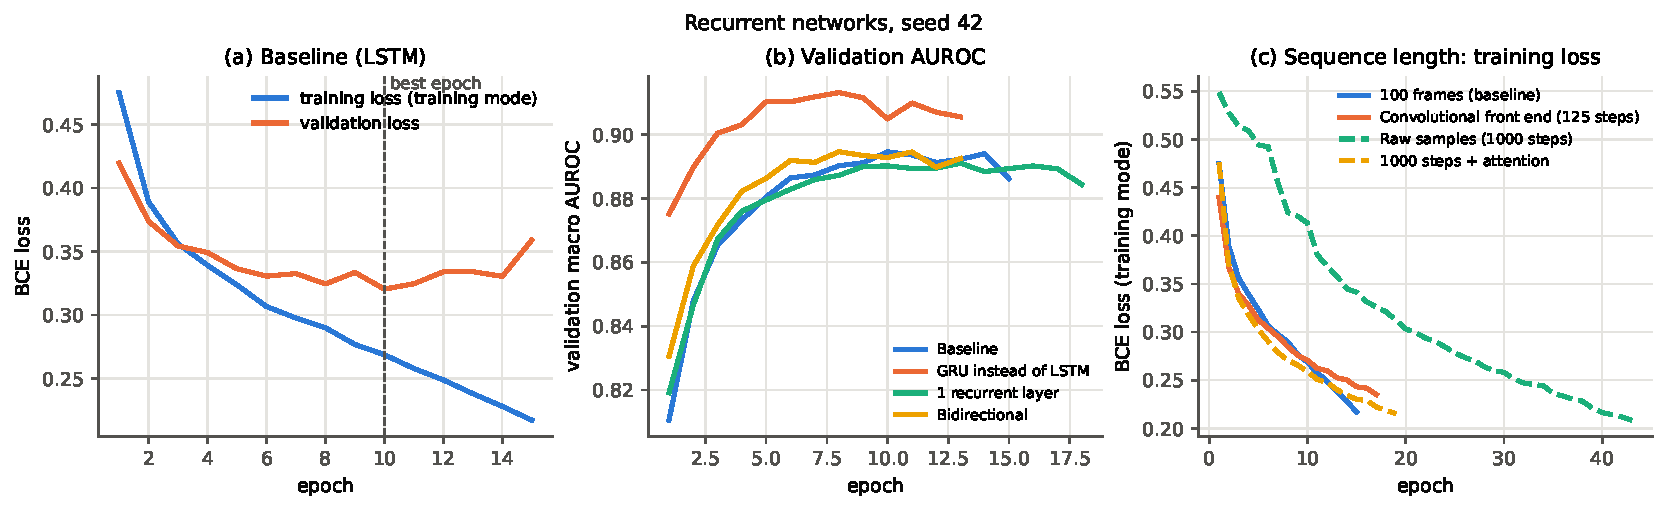
\includegraphics[width=\textwidth,height=0.42\textheight,keepaspectratio]{figures/rnn_curves.pdf}
\caption[Recurrent networks: learning curves]{Recurrent networks, seed 42. (a) LSTM baseline losses. (b) Validation macro AUROC of the baseline, GRU, one recurrent layer and bidirectional LSTM. (c) Training loss with 100 frames, the convolutional front end, 1000 raw steps and 1000 steps with attention.}
\label{fig:rnn_curves}
\end{figure}

% Shared float (common/make_floats.py). Figure: figures/transformer_curves.pdf
\begin{figure}[htbp]
\centering
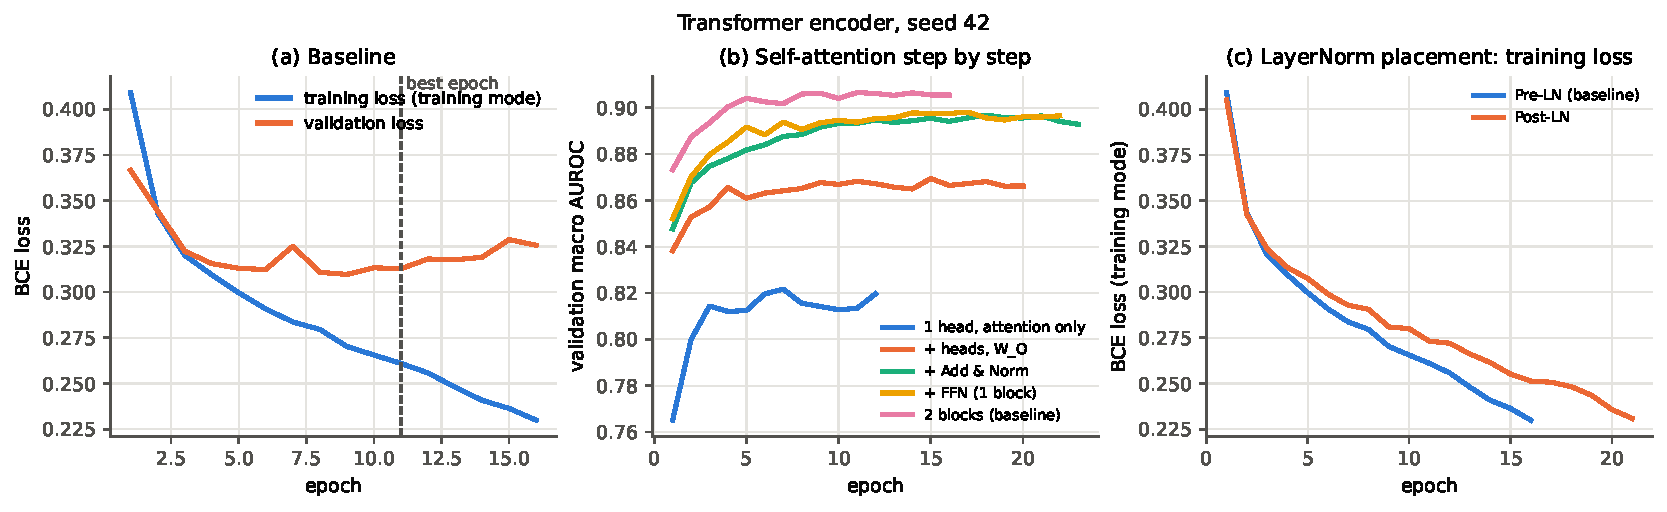
\includegraphics[width=\textwidth,height=0.42\textheight,keepaspectratio]{figures/transformer_curves.pdf}
\caption[Transformer: learning curves and self-attention step by step]{Transformer encoder, seed 42. (a) Baseline losses. (b) Self-attention step by step: validation macro AUROC from one single-head attention layer to two full blocks. (c) Training loss with Pre-LN and Post-LN.}
\label{fig:transformer_curves}
\end{figure}


\subsection{Evaluation code}

\paragraph{Metrics.} Probabilities are \texttt{sigmoid(logits)}, computed outside the model. The AUROC of
each class comes from scikit-learn and the macro AUROC is their plain mean. For F1, each class gets the
threshold of the grid 0.01--0.99 that maximises its F1 on validation (lowest threshold on ties), and the
same thresholds are applied to test.

\paragraph{Patient bootstrap.} Listing~\ref{lst:boot} draws the resamples. Patients, not records, are drawn
with replacement; \texttt{np.bincount} counts how many times each patient was drawn and \texttt{np.repeat}
repeats all of that patient's records as many times. Because the draws depend only on the patient
identifiers and the seed, every model evaluated on the same split sees exactly the same resamples. A
resample in which a class has no positive or no negative record (AUROC undefined) is discarded and counted
in the log.

\lstinputlisting[firstnumber=101,caption={Patient-level bootstrap resamples (\texttt{src/metrics.py}).},label={lst:boot}]{common/code/patient_bootstrap.py}

\paragraph{Paired difference.} Listing~\ref{lst:paired} uses those same resamples to compute the interval of
the difference in macro AUROC between two models on the same records. It needs both models' predictions in
the same record order, which is why every run saves its probabilities with the record and patient
identifiers, and why \texttt{python -m src.compare RUN\_A RUN\_B} refuses two runs whose records differ.

\lstinputlisting[firstnumber=164,caption={Paired bootstrap difference of two models (\texttt{src/metrics.py}).},label={lst:paired}]{common/code/paired_bootstrap.py}

\subsection{Run logs and numbers of the reports}

Every run is named \texttt{<model>\_<tag>\_s<seed>\_<date-time>} and writes three files: a JSON log
(configuration, seed, data description, curves, best epoch, results per split with intervals, parameter
counts, software versions, git commit and whether the code under \texttt{src/} had uncommitted changes), the
predictions (\texttt{.npz}) and the best weights (not committed). The test fold is evaluated only with
\texttt{--final}, and a second final run with the same model, tag and seed is refused.

\texttt{report/runs.json} maps a short alias to each log or block summary allowed in a report, and
\texttt{report/make\_numbers.py} turns every scalar of those logs into a LaTeX macro. Macro names can only
contain letters, so the key is cut at underscores and at letter--digit boundaries and digits are spelled
out: the mean test macro AUROC of the final RNN is \verb|\rnnFinalTestMacroAurocMean| and prints
\rnnFinalTestMacroAurocMean{}. A report therefore cannot contain a number that is not in a log, and a
re-run updates every table and sentence at once.

% =====================================================================
% 4. Architectures in PyTorch (MLLB, Maria Martinez)
% Own blocks in depth: src/models/rnn.py (T11), src/models/attention.py and
% src/models/transformer.py (T12). Dense and CNN (Oriana) summarised.
% =====================================================================
\section{Architectures in PyTorch}\label{sec:mllb-arch}

This section explains how my models are implemented, with the PyTorch details that matter for them; the
theory and the analysis of the results are in my PRDL report. All models map (batch, 12, 1000) to five
logits, and my models end with the head of the CNN baseline: dropout 0.5 and one linear layer.

\subsection{Dense network and CNN (Oriana's blocks)}

Oriana's dense network flattens the record (\texttt{nn.Flatten}) and applies fully connected layers with
batch norm, ReLU and dropout. Her CNN stacks residual blocks of \texttt{Conv1d}, batch norm and ReLU with a
$1\times1$ convolution on the shortcut when the number of channels changes, and ends with global average
pooling. I reused the first three of her convolutional blocks, unchanged, as the front end of my best
recurrent model.

\subsection{Recurrent networks}

\paragraph{From a signal to a sequence.} \texttt{nn.LSTM(batch\_first=True)} expects (batch, time,
features), the opposite axis order of \texttt{Conv1d} (batch, channels, time). Listing~\ref{lst:rnnseq}
builds the sequence. For frames, \texttt{reshape(b, c, t, frame)} cuts each lead into $t$ frames,
\texttt{permute(0, 2, 1, 3)} moves time before the leads, and the last \texttt{reshape} flattens the 12
leads $\times$ 10 samples of each frame into one vector of 120 numbers; a test checks this element by
element. For the convolutional front end, the output of the CNN blocks (batch, 128, 125) is simply
permuted to (batch, 125, 128). No padding is needed, because every record has exactly 1000 samples.

\lstinputlisting[firstnumber=152,caption={From the signal to the sequence read by the RNN, and the final state (\texttt{src/models/rnn.py}).},label={lst:rnnseq}]{common/code/rnn_sequence_encode.py}

\paragraph{What \texttt{nn.LSTM} returns.} The second part of Listing~\ref{lst:rnnseq} handles the outputs:
\begin{itemize}[leftmargin=1.2em,itemsep=1pt]
  \item \texttt{out} has the hidden states of the top layer at every step, (batch, $T$, hidden) or
        (batch, $T$, 2 $\times$ hidden) if bidirectional.
  \item The LSTM also returns \texttt{(h\_n, c\_n)}, the final hidden and cell states of every layer and
        direction; the GRU returns only \texttt{h\_n}, because it has no cell state. The code checks for a
        tuple so that one class handles both cells.
  \item For a unidirectional network, \texttt{h\_n[-1]} (top layer) equals \texttt{out[:, -1, :]}.
  \item For a bidirectional network the final summary is the concatenation of \texttt{h\_n[-2]}, the
        forward direction, which has read the record from left to right, and \texttt{h\_n[-1]}, the
        backward direction, which has read it from right to left. The backward final state is at
        \texttt{out[:, 0, hidden:]}, not at \texttt{out[:, -1, :]}: taking the last row of \texttt{out}
        would pair the forward summary with a backward state that has read only one step. A test checks
        both facts.
\end{itemize}
Two more details. The \texttt{dropout} argument of \texttt{nn.LSTM} only acts between stacked layers, so it is
left at 0 and dropout is applied to the summary vector before the classifier. And a test checks causality:
in a unidirectional network, changing the second half of the record leaves the states of the first half
unchanged.

\paragraph{Attention pooling.} Listing~\ref{lst:attnpool} computes the scores, the weights and the context
vector. \texttt{nn.Linear} acts on the last axis, with the same weights at every time step, so it is already
``time distributed''. The softmax is taken over time (\texttt{dim=1}), and \texttt{torch.bmm} multiplies the
weights (batch, 1, $T$) by the states (batch, $T$, $d$) to give the context vector (batch, 1, $d$). The weights
are returned too, for the figures.

\lstinputlisting[firstnumber=66,caption={Attention scores and context vector over the RNN states (\texttt{src/models/rnn.py}).},label={lst:attnpool}]{common/code/attention_pooling.py}

\paragraph{Gradients with respect to the input.} The sensitivity analysis needs
$\partial\,\mathrm{logit}/\partial x$: the input tensor gets \texttt{requires\_grad\_(True)} and
\texttt{torch.autograd.grad} computes the gradient of the summed logit. In eval mode the records of a batch do
not interact, so the gradient of the sum gives each record's gradient. This is computed on the CPU, because
cuDNN only runs the backward pass of an RNN in training mode, where dropout would change the result.

\subsection{Self-attention and the Transformer, written by hand}

I wrote multi-head self-attention myself instead of using \file{nn.MultiheadAttention} or
\file{nn.TransformerEncoderLayer}, so that every step can be explained and the attention weights are
available; a test checks that my module gives the same output as \texttt{nn.MultiheadAttention} with the
same weights, with and without a causal mask.

\paragraph{Patches as tokens.} Listing~\ref{lst:patches} cuts the record into patches with the same
reshape and permute as the RNN frames, so both models see the same 100 steps. One linear layer embeds each
patch; it is exactly a \texttt{Conv1d} with kernel and stride equal to the patch length (checked by a test).
An optional CLS token is an \texttt{nn.Parameter} of shape (1, 1, $d$), expanded to the batch and
concatenated in front of the patches. The sinusoidal positional encoding is registered as a buffer with
\texttt{persistent=False}: it moves to the GPU with the model, the optimiser does not change it, and it is
not saved in the checkpoint, because it is rebuilt when the model is created.

\lstinputlisting[firstnumber=96,caption={Patch tokens, CLS token and positional encoding (\texttt{src/models/transformer.py}).},label={lst:patches}]{common/code/patch_tokens.py}

\paragraph{Scaled dot-product attention.} In Listing~\ref{lst:attn}, \texttt{q @ k.transpose(-2, -1)} computes
all query--key dot products at once, shape (\ldots, $T$, $T$); they are divided by $\sqrt{d_k}$, the dimension
of one head, not of the model. Masked scores are set to $-\infty$ with \texttt{masked\_fill} before the
softmax, so their weights are exactly 0; the softmax is over the keys (last axis), so each query's weights
sum to 1. My classifier does not use the mask, but Oriana's generator reuses this same function with the
causal mask of \texttt{causal\_mask}, a lower-triangular boolean matrix.

\lstinputlisting[firstnumber=29,caption={Causal mask and scaled dot-product attention (\texttt{src/models/attention.py}).},label={lst:attn}]{common/code/causal_attention.py}

\paragraph{Splitting into heads.} Listing~\ref{lst:mhsa} projects the input into queries, keys and values
with three bias-free linear layers and splits $d_\text{model}$ into heads: \texttt{view(b, t, heads,
head\_dim)} cuts the last axis and \texttt{permute(0, 2, 1, 3)} moves the heads before time, giving (batch,
heads, $T$, head\_dim), so the attention runs on every head in parallel. Joining the heads back needs
\texttt{reshape}, not \texttt{view}: after \texttt{permute} the tensor is no longer contiguous in memory and
\texttt{view} would fail. $W_O$ then mixes the concatenated heads.

\lstinputlisting[firstnumber=93,caption={Multi-head self-attention: heads, attention and $W_O$ (\texttt{src/models/attention.py}).},label={lst:mhsa}]{common/code/mhsa_split_forward.py}

\paragraph{Pre-LN and Post-LN in one function.} Listing~\ref{lst:sublayer} applies one sub-layer with its
skip connection and LayerNorm. With Pre-LN the input is normalised before the sub-layer and the result is
added to the unnormalised residual stream; with Post-LN the LayerNorm is applied after the addition. The
flags \texttt{residual}, \texttt{ffn} and \texttt{out\_proj} remove components, which is how the five models of
the step-by-step study are built from the same class. Because Pre-LN leaves the residual stream
unnormalised after the last block, the encoder applies a final LayerNorm. The attention maps are returned by
every block and collected in eval mode on the CPU.

\lstinputlisting[firstnumber=173,caption={One sub-layer with skip connection and LayerNorm (\texttt{src/models/attention.py}).},label={lst:sublayer}]{common/code/block_sublayer.py}

\subsection{Results of my blocks in brief}

The final models are an LSTM with a convolutional front end (\texttt{conv},
\rnnFinalTestMacroAurocMean{}~$\pm$~\rnnFinalTestMacroAurocSd{} on test), an LSTM with attention over 1000 raw
steps (\texttt{raw\_attn}, \rnnAttnfinalTestMacroAurocMean{}~$\pm$~\rnnAttnfinalTestMacroAurocSd{}) and a
two-block Transformer without positional encoding (\texttt{no\_pos},
\transformerFinalTestMacroAurocMean{}~$\pm$~\transformerFinalTestMacroAurocSd{}), against
\cnnFinalTestMacroAurocMean{} for the CNN (Table~\ref{tab:comparison_final}). The implementation points that
mattered most for these results were the axis order of the sequence (any mistake there would silently mix
leads and time), reading all hidden states instead of the last one, and the shapes of the attention heads.

% =====================================================================
% 5. Learning strategies and generator: implementation (MLLB, Maria Martinez)
% Shared T13, T14, T24 (DECISIONS D20, block note 08); generator (Oriana,
% T23, D19, block note 13), summarised and attributed.
% =====================================================================
\section{Learning strategies and generator: implementation}\label{sec:mllb-strategies}

\subsection{Transfer from the self-supervised generator}

Oriana and I ran the transfer experiments together. The pre-trained network is Oriana's ECG-GPT
(Section~\ref{sec:mllb-generator}); its \texttt{record\_features} method returns one vector of 128 numbers
per record, the mean of the outputs of its final LayerNorm over the windows that cover lead II. Listing~\ref{lst:transfer}
puts a new head on top.

\lstinputlisting[firstnumber=185,caption={Generator backbone with a new classification head (\texttt{src/transfer.py}).},label={lst:transfer}]{common/code/transfer_classifier.py}

\begin{itemize}[leftmargin=1.2em,itemsep=1pt]
  \item \textbf{Freezing.} For the linear probe every backbone parameter gets \texttt{requires\_grad\_(False)};
        since the optimiser only receives trainable parameters, the backbone cannot change.
        Freezing the weights is not enough, though: the loop calls \texttt{model.train()} every epoch, which
        would switch on the backbone's dropout and give a different vector for the same record each time.
        The class therefore overrides \texttt{train()} to keep the frozen backbone in eval mode.
  \item \textbf{Caching the features.} With a frozen backbone each record always gives the same vector, so
        the vectors are computed once per checkpoint and the head is trained on them; a test checks that this
        is the same model as passing the tokens every epoch.
  \item \textbf{Fine-tuning.} Everything trainable, with a learning rate of $10^{-4}$ instead of $10^{-3}$, as in
        the class transfer-learning notebook \cite{course_nb_transfer}: at the start the new head is random and
        its large gradients flow into the pre-trained layers. The ablation at $10^{-3}$ showed that this was
        not essential here.
  \item \textbf{Memory.} One record is four windows of 250 tokens, so the activations kept for
        backpropagation grow fast; the transfer runs use batches of 32 records instead of 64, the same for
        every transfer configuration.
  \item \textbf{The 10\,\% subset} is drawn by patient with a generator seeded by the run's seed, and is the
        same for the three strategies of that seed, so they are compared on the same labelled records.
\end{itemize}
Results (Table~\ref{tab:transfer_main}): fine-tuning reached
\transferTestAurocMeanFinetuneFOneZeroZero{} on test with all the labels and
\transferTestAurocMeanFinetuneFOneZero{} with 10\,\%, against \transferTestAurocMeanScratchFOneZeroZero{}
and \transferTestAurocMeanScratchFOneZero{} from scratch.

% Shared float (common/make_floats.py). Table: tables/transfer_main.tex
\begin{table}[htbp]
\centering
\caption[Transfer from the ECG-GPT: main results]{ECG-GPT reused for the five superclasses (lead II): the three strategies with 100\,\% and 10\,\% of the training labels (mean $\pm$ SD over seeds 42--44).}
\label{tab:transfer_main}
\small
\begin{adjustbox}{max width=\textwidth}
% Generated by src/transfer_experiments.py from results/logs/transfer_summary.json.
% Needs report/numbers.tex (alias "transfer") and booktabs.
\begin{tabular}{llrrccc}
\toprule
Labels & Strategy & Train.\ param. & Train records & Val.\ macro AUROC & Test macro AUROC & Test macro F1 \\
\midrule
100\% & From scratch & \transferParamsScratchFOneZeroZero{} & \transferNTrainScratchFOneZeroZero{} & \transferValAurocMeanScratchFOneZeroZero{} $\pm$ \transferValAurocSdScratchFOneZeroZero{} & \transferTestAurocMeanScratchFOneZeroZero{} $\pm$ \transferTestAurocSdScratchFOneZeroZero{} & \transferTestFOneMeanScratchFOneZeroZero{} $\pm$ \transferTestFOneSdScratchFOneZeroZero{} \\
100\% & Linear probe (frozen) & \transferParamsProbeFOneZeroZero{} & \transferNTrainProbeFOneZeroZero{} & \transferValAurocMeanProbeFOneZeroZero{} $\pm$ \transferValAurocSdProbeFOneZeroZero{} & \transferTestAurocMeanProbeFOneZeroZero{} $\pm$ \transferTestAurocSdProbeFOneZeroZero{} & \transferTestFOneMeanProbeFOneZeroZero{} $\pm$ \transferTestFOneSdProbeFOneZeroZero{} \\
100\% & Fine-tuning & \transferParamsFinetuneFOneZeroZero{} & \transferNTrainFinetuneFOneZeroZero{} & \transferValAurocMeanFinetuneFOneZeroZero{} $\pm$ \transferValAurocSdFinetuneFOneZeroZero{} & \transferTestAurocMeanFinetuneFOneZeroZero{} $\pm$ \transferTestAurocSdFinetuneFOneZeroZero{} & \transferTestFOneMeanFinetuneFOneZeroZero{} $\pm$ \transferTestFOneSdFinetuneFOneZeroZero{} \\
\addlinespace
10\% & From scratch & \transferParamsScratchFOneZero{} & \transferNTrainScratchFOneZero{} & \transferValAurocMeanScratchFOneZero{} $\pm$ \transferValAurocSdScratchFOneZero{} & \transferTestAurocMeanScratchFOneZero{} $\pm$ \transferTestAurocSdScratchFOneZero{} & \transferTestFOneMeanScratchFOneZero{} $\pm$ \transferTestFOneSdScratchFOneZero{} \\
10\% & Linear probe (frozen) & \transferParamsProbeFOneZero{} & \transferNTrainProbeFOneZero{} & \transferValAurocMeanProbeFOneZero{} $\pm$ \transferValAurocSdProbeFOneZero{} & \transferTestAurocMeanProbeFOneZero{} $\pm$ \transferTestAurocSdProbeFOneZero{} & \transferTestFOneMeanProbeFOneZero{} $\pm$ \transferTestFOneSdProbeFOneZero{} \\
10\% & Fine-tuning & \transferParamsFinetuneFOneZero{} & \transferNTrainFinetuneFOneZero{} & \transferValAurocMeanFinetuneFOneZero{} $\pm$ \transferValAurocSdFinetuneFOneZero{} & \transferTestAurocMeanFinetuneFOneZero{} $\pm$ \transferTestAurocSdFinetuneFOneZero{} & \transferTestFOneMeanFinetuneFOneZero{} $\pm$ \transferTestFOneSdFinetuneFOneZero{} \\
\bottomrule
\end{tabular}

\end{adjustbox}
\end{table}


\subsection{Single lead and zero-shot}

The single-lead ablation needed no new model code: every architecture takes \texttt{n\_leads} as an
argument, so the final model of each family was rebuilt with \texttt{n\_leads=1} and its 12-lead arguments,
and fed lead II only. Runs are named \texttt{onelead\_*} so that they can never be mixed with the 12-lead
runs that each block's summary reads.

The zero-shot experiment loads CLIP ViT-B/32 with OpenAI's weights through \texttt{open\_clip}, as
\texttt{ViT-B-32-quickgelu}: OpenAI trained this model with the QuickGELU activation, and the plain
\texttt{ViT-B-32} configuration of \texttt{open\_clip} uses GELU, so it would not have been exactly the model
of the class notebook \cite{course_nb_clip}. Each ECG is drawn as a $224 \times 224$ image, the size CLIP
expects, so its preprocessing does not crop it. The first run failed because the image features had been
moved to the CPU and the text features stayed on the GPU; the fix is described in
Appendix~\ref{app:ai-code}.

\subsection{The generator (Oriana's block)}\label{sec:mllb-generator}

The generator was implemented by Oriana; it reuses my attention module with \texttt{causal=True}. Lead II is
quantised on a microvolt grid into integer tokens; the training windows of 250 tokens are cut at random
positions inside \texttt{\_\_getitem\_\_}, with a NumPy generator seeded by the run, so the draws are
reproducible with \texttt{num\_workers=0}. The model returns logits of shape (batch, $T$, $V$), which must
be flattened to (batch $\cdot$ $T$, $V$) before \texttt{cross\_entropy}, otherwise PyTorch reads $T$ as the
class axis. Generation runs under \texttt{torch.no\_grad()} in eval mode, samples the next token with
\texttt{torch.multinomial} and a seeded generator, and only computes the output layer at the last position.
Its main implementation lesson concerns memory: the attention matrix grows with the square of the
context, and generating with long contexts ran out of the 4\,GB of the GPU until the batch was reduced in
proportion.

% =====================================================================
% 6. Code distribution and reproduction (MLLB, Maria Martinez)
% README, DECISIONS D5, D11, D14.
% =====================================================================
\section{Code distribution and reproduction}\label{sec:code}

\subsection{Repository}

All code, logs, tables and figures are in the public repository
\url{https://github.com/orianafe16/ptbxl-DL}. The raw data and the cache are not committed: they are
downloaded from PhysioNet, checked against the published checksums and rebuilt. Checkpoints are not
committed either; predictions and logs are.

\begin{table}[htbp]
\centering
\caption{Structure of the repository and the files of my blocks.}
\label{tab:repo}
\small
\begin{tabularx}{\textwidth}{>{\raggedright\arraybackslash}p{4.2cm} >{\raggedright\arraybackslash}X}
\toprule
\textbf{Path} & \textbf{Content} \\
\midrule
\file{src/config.py}, \file{src/data.py}, \file{src/prepare_data.py}, \file{src/dataset.py} & Paths and settings; integrity check, labels and cache; split, normalisation, \texttt{Dataset} and \texttt{DataLoader}s (mine) \\
\file{src/metrics.py}, \file{src/tasks.py}, \file{src/train.py}, \file{src/runlog.py}, \file{src/compare.py} & Metrics and bootstrap, tasks, training loop, run logs, paired comparison (evaluation mine, loop shared) \\
\file{src/models/rnn.py}, \file{src/rnn_experiments.py} & LSTM, GRU and attention pooling; ablations, final models, report (mine) \\
\file{src/models/attention.py}, \file{src/models/transformer.py}, \file{src/transformer_experiments.py} & Hand-written attention, encoder blocks, Transformer classifier; ablations, final model, report (mine) \\
\file{src/models/dense.py}, \file{src/models/cnn.py}, generative and learning-strategy modules & Oriana's blocks and the shared area-2 experiments \\
\file{tests/} & Automated tests (pytest) of every module \\
\file{results/logs/}, \file{results/predictions/} & One JSON log and one prediction file per run; one summary per block \\
\file{report/} & Tables and figures generated by the code, \file{runs.json}, \file{make_numbers.py}, \file{numbers.tex}, these reports \\
\file{docs/} & Decisions log, task plan, AI usage log, one note per block, literature quotes \\
\bottomrule
\end{tabularx}
\end{table}

\subsection{Reproducing my results}

From a clean copy, with the Python environment of \file{requirements.txt} and the PTB-XL files in
\file{data/raw/ptbxl/}:
\begin{lstlisting}[language=bash,numbers=none,caption={Commands to reproduce my blocks.}]
python -m src.prepare_data                  # check the files, build the cache
python -m pytest -q tests                   # tests
python -m src.rnn_experiments estimate      # time per epoch on this GPU
python -m src.rnn_experiments all --fast    # smoke test (not reported)
python -m src.rnn_experiments all           # ablations + final models + report
python -m src.transformer_experiments estimate
python -m src.transformer_experiments all --fast
python -m src.transformer_experiments all
python report/make_numbers.py               # report/numbers.tex
\end{lstlisting}
\texttt{run} and \texttt{final} skip what has already been run, so an interrupted block can be resumed. The
cost of each configuration on the laptop is in Table~\ref{tab:mllb-cost}. Reproduction has three levels.
(1) From a clean clone, without data or GPU, the test suite runs on synthetic data, and
\file{report/make_numbers.py} rebuilds \file{numbers.tex} from the committed logs, which is all the reports
need; we checked that it gives exactly the same macros. (2) With the PTB-XL files and the checkpoints,
which are kept outside git and backed up separately, the \texttt{report} step of each block rebuilds its
tables and figures; the interpretation figures (attention weights, input sensitivity) need the
checkpoints. (3) Retraining repeats the runs; on a GPU, results can differ slightly from the logged ones,
because PyTorch's fully deterministic mode is not enabled.

\subsection{Tests}

The tests run on a CPU with synthetic data, so they need neither the GPU nor the dataset (the tests on the
real cache are skipped when it is missing). For my blocks they check, among other things:
\begin{itemize}[leftmargin=1.2em,itemsep=1pt]
  \item the data: split by fold, exclusion of records without a superclass, training-only statistics,
        class counts against the PhysioNet table, no patient in two splits;
  \item the evaluation: metrics on toy cases with known answers, patients kept together in the bootstrap,
        identical resamples for the same seed, a refused second final run;
  \item the recurrent models: framing element by element, LSTM and GRU states, the bidirectional final
        state, causality, the attention weights and the bound of the notebook score, the input sensitivity;
  \item the attention models: equality with \texttt{nn.MultiheadAttention}, the causal mask, the order of
        Pre-LN and Post-LN, the patch embedding equal to a \texttt{Conv1d}, the parameter count, the order
        invariance without positions, and the single-layer model equal to an attention pooling;
  \item for both blocks, the selection rule and the whole pipeline on a small synthetic cache.
\end{itemize}

\subsection{Traceability of the final results}

Table~\ref{tab:comparison_final} is the final comparison of the project, generated by
\texttt{python -m src.comparison report} from the summaries of every block. Each value is a macro, and each
macro can be traced to one key of one log listed in \file{report/runs.json}; each log records the commit of
the code that produced it and whether that code had uncommitted changes. The runs of my blocks were made
at committed versions of the code (commits \texttt{cae71d5} for the recurrent block and \texttt{f11e501} for
the Transformer). The only values typed by hand are the published benchmark rows, stored in
\file{report/published.json} with file, page and quote.

% Shared float (common/make_floats.py). Table: tables/comparison_final.tex
\begin{table}[htbp]
\centering
\caption[Final comparison (test)]{Final comparison on the test fold. Mean $\pm$ SD over seeds; interval: 95\,\% patient bootstrap of the first seed. Published rows: macro AUC of the superclass task in Table~I of \cite{strodthoff2021deep}, obtained in a different setting (described in the text).}
\label{tab:comparison_final}
\small
\begin{adjustbox}{max width=\textwidth}
% Generated by src/comparison.py from results/logs/comparison_summary.json.
% Mean +- SD over seeds (one run: no SD); CI = 95% patient bootstrap of the first seed. Needs alias "comparison".
\begin{tabular}{lcrrccc}
\toprule
Model & Labels & Train.\ param. & Seeds & Test macro AUROC & First seed [95\% CI] & Test macro F1 \\
\midrule
\multicolumn{7}{l}{\textit{12 leads}} \\
\quad Trivial (lead mean and SD) & 100\% & \comparisonParamsTrivial{} & \comparisonNSeedsTrivial{} & \comparisonTestAurocMeanTrivial{} & \comparisonTestAurocFirstTrivial{} [\comparisonTestAurocLoFirstTrivial{}, \comparisonTestAurocHiFirstTrivial{}] & \comparisonTestFOneMeanTrivial{} \\
\quad Dense & 100\% & \comparisonParamsTwelveDense{} & \comparisonNSeedsTwelveDense{} & \comparisonTestAurocMeanTwelveDense{} $\pm$ \comparisonTestAurocSdTwelveDense{} & \comparisonTestAurocFirstTwelveDense{} [\comparisonTestAurocLoFirstTwelveDense{}, \comparisonTestAurocHiFirstTwelveDense{}] & \comparisonTestFOneMeanTwelveDense{} $\pm$ \comparisonTestFOneSdTwelveDense{} \\
\quad CNN & 100\% & \comparisonParamsTwelveCnn{} & \comparisonNSeedsTwelveCnn{} & \comparisonTestAurocMeanTwelveCnn{} $\pm$ \comparisonTestAurocSdTwelveCnn{} & \comparisonTestAurocFirstTwelveCnn{} [\comparisonTestAurocLoFirstTwelveCnn{}, \comparisonTestAurocHiFirstTwelveCnn{}] & \comparisonTestFOneMeanTwelveCnn{} $\pm$ \comparisonTestFOneSdTwelveCnn{} \\
\quad RNN & 100\% & \comparisonParamsTwelveRnn{} & \comparisonNSeedsTwelveRnn{} & \comparisonTestAurocMeanTwelveRnn{} $\pm$ \comparisonTestAurocSdTwelveRnn{} & \comparisonTestAurocFirstTwelveRnn{} [\comparisonTestAurocLoFirstTwelveRnn{}, \comparisonTestAurocHiFirstTwelveRnn{}] & \comparisonTestFOneMeanTwelveRnn{} $\pm$ \comparisonTestFOneSdTwelveRnn{} \\
\quad RNN + attention & 100\% & \comparisonParamsTwelveRnnattn{} & \comparisonNSeedsTwelveRnnattn{} & \comparisonTestAurocMeanTwelveRnnattn{} $\pm$ \comparisonTestAurocSdTwelveRnnattn{} & \comparisonTestAurocFirstTwelveRnnattn{} [\comparisonTestAurocLoFirstTwelveRnnattn{}, \comparisonTestAurocHiFirstTwelveRnnattn{}] & \comparisonTestFOneMeanTwelveRnnattn{} $\pm$ \comparisonTestFOneSdTwelveRnnattn{} \\
\quad Transformer & 100\% & \comparisonParamsTwelveTransformer{} & \comparisonNSeedsTwelveTransformer{} & \comparisonTestAurocMeanTwelveTransformer{} $\pm$ \comparisonTestAurocSdTwelveTransformer{} & \comparisonTestAurocFirstTwelveTransformer{} [\comparisonTestAurocLoFirstTwelveTransformer{}, \comparisonTestAurocHiFirstTwelveTransformer{}] & \comparisonTestFOneMeanTwelveTransformer{} $\pm$ \comparisonTestFOneSdTwelveTransformer{} \\
\addlinespace
\multicolumn{7}{l}{\textit{Lead II only (T14)}} \\
\quad Dense & 100\% & \comparisonParamsOneleadDense{} & \comparisonNSeedsOneleadDense{} & \comparisonTestAurocMeanOneleadDense{} $\pm$ \comparisonTestAurocSdOneleadDense{} & \comparisonTestAurocFirstOneleadDense{} [\comparisonTestAurocLoFirstOneleadDense{}, \comparisonTestAurocHiFirstOneleadDense{}] & \comparisonTestFOneMeanOneleadDense{} $\pm$ \comparisonTestFOneSdOneleadDense{} \\
\quad CNN & 100\% & \comparisonParamsOneleadCnn{} & \comparisonNSeedsOneleadCnn{} & \comparisonTestAurocMeanOneleadCnn{} $\pm$ \comparisonTestAurocSdOneleadCnn{} & \comparisonTestAurocFirstOneleadCnn{} [\comparisonTestAurocLoFirstOneleadCnn{}, \comparisonTestAurocHiFirstOneleadCnn{}] & \comparisonTestFOneMeanOneleadCnn{} $\pm$ \comparisonTestFOneSdOneleadCnn{} \\
\quad RNN & 100\% & \comparisonParamsOneleadRnn{} & \comparisonNSeedsOneleadRnn{} & \comparisonTestAurocMeanOneleadRnn{} $\pm$ \comparisonTestAurocSdOneleadRnn{} & \comparisonTestAurocFirstOneleadRnn{} [\comparisonTestAurocLoFirstOneleadRnn{}, \comparisonTestAurocHiFirstOneleadRnn{}] & \comparisonTestFOneMeanOneleadRnn{} $\pm$ \comparisonTestFOneSdOneleadRnn{} \\
\quad RNN + attention & 100\% & \comparisonParamsOneleadRnnattn{} & \comparisonNSeedsOneleadRnnattn{} & \comparisonTestAurocMeanOneleadRnnattn{} $\pm$ \comparisonTestAurocSdOneleadRnnattn{} & \comparisonTestAurocFirstOneleadRnnattn{} [\comparisonTestAurocLoFirstOneleadRnnattn{}, \comparisonTestAurocHiFirstOneleadRnnattn{}] & \comparisonTestFOneMeanOneleadRnnattn{} $\pm$ \comparisonTestFOneSdOneleadRnnattn{} \\
\quad Transformer & 100\% & \comparisonParamsOneleadTransformer{} & \comparisonNSeedsOneleadTransformer{} & \comparisonTestAurocMeanOneleadTransformer{} $\pm$ \comparisonTestAurocSdOneleadTransformer{} & \comparisonTestAurocFirstOneleadTransformer{} [\comparisonTestAurocLoFirstOneleadTransformer{}, \comparisonTestAurocHiFirstOneleadTransformer{}] & \comparisonTestFOneMeanOneleadTransformer{} $\pm$ \comparisonTestFOneSdOneleadTransformer{} \\
\addlinespace
\multicolumn{7}{l}{\textit{Lead II, ECG-GPT transfer (T13)}} \\
\quad ECG-GPT, from scratch & 100\% & \comparisonParamsScratchFOneZeroZero{} & \comparisonNSeedsScratchFOneZeroZero{} & \comparisonTestAurocMeanScratchFOneZeroZero{} $\pm$ \comparisonTestAurocSdScratchFOneZeroZero{} & \comparisonTestAurocFirstScratchFOneZeroZero{} [\comparisonTestAurocLoFirstScratchFOneZeroZero{}, \comparisonTestAurocHiFirstScratchFOneZeroZero{}] & \comparisonTestFOneMeanScratchFOneZeroZero{} $\pm$ \comparisonTestFOneSdScratchFOneZeroZero{} \\
\quad ECG-GPT, linear probe (frozen) & 100\% & \comparisonParamsProbeFOneZeroZero{} & \comparisonNSeedsProbeFOneZeroZero{} & \comparisonTestAurocMeanProbeFOneZeroZero{} $\pm$ \comparisonTestAurocSdProbeFOneZeroZero{} & \comparisonTestAurocFirstProbeFOneZeroZero{} [\comparisonTestAurocLoFirstProbeFOneZeroZero{}, \comparisonTestAurocHiFirstProbeFOneZeroZero{}] & \comparisonTestFOneMeanProbeFOneZeroZero{} $\pm$ \comparisonTestFOneSdProbeFOneZeroZero{} \\
\quad ECG-GPT, fine-tuning & 100\% & \comparisonParamsFinetuneFOneZeroZero{} & \comparisonNSeedsFinetuneFOneZeroZero{} & \comparisonTestAurocMeanFinetuneFOneZeroZero{} $\pm$ \comparisonTestAurocSdFinetuneFOneZeroZero{} & \comparisonTestAurocFirstFinetuneFOneZeroZero{} [\comparisonTestAurocLoFirstFinetuneFOneZeroZero{}, \comparisonTestAurocHiFirstFinetuneFOneZeroZero{}] & \comparisonTestFOneMeanFinetuneFOneZeroZero{} $\pm$ \comparisonTestFOneSdFinetuneFOneZeroZero{} \\
\quad ECG-GPT, from scratch & 10\% & \comparisonParamsScratchFOneZero{} & \comparisonNSeedsScratchFOneZero{} & \comparisonTestAurocMeanScratchFOneZero{} $\pm$ \comparisonTestAurocSdScratchFOneZero{} & \comparisonTestAurocFirstScratchFOneZero{} [\comparisonTestAurocLoFirstScratchFOneZero{}, \comparisonTestAurocHiFirstScratchFOneZero{}] & \comparisonTestFOneMeanScratchFOneZero{} $\pm$ \comparisonTestFOneSdScratchFOneZero{} \\
\quad ECG-GPT, linear probe (frozen) & 10\% & \comparisonParamsProbeFOneZero{} & \comparisonNSeedsProbeFOneZero{} & \comparisonTestAurocMeanProbeFOneZero{} $\pm$ \comparisonTestAurocSdProbeFOneZero{} & \comparisonTestAurocFirstProbeFOneZero{} [\comparisonTestAurocLoFirstProbeFOneZero{}, \comparisonTestAurocHiFirstProbeFOneZero{}] & \comparisonTestFOneMeanProbeFOneZero{} $\pm$ \comparisonTestFOneSdProbeFOneZero{} \\
\quad ECG-GPT, fine-tuning & 10\% & \comparisonParamsFinetuneFOneZero{} & \comparisonNSeedsFinetuneFOneZero{} & \comparisonTestAurocMeanFinetuneFOneZero{} $\pm$ \comparisonTestAurocSdFinetuneFOneZero{} & \comparisonTestAurocFirstFinetuneFOneZero{} [\comparisonTestAurocLoFirstFinetuneFOneZero{}, \comparisonTestAurocHiFirstFinetuneFOneZero{}] & \comparisonTestFOneMeanFinetuneFOneZero{} $\pm$ \comparisonTestFOneSdFinetuneFOneZero{} \\
\addlinespace
\multicolumn{7}{l}{\textit{Lead II, zero-shot (T24)}} \\
\quad CLIP ViT-B/32, zero-shot & 0\% & --- & \comparisonNSeedsZeroshot{} & \comparisonTestAurocMeanZeroshot{} & \comparisonTestAurocFirstZeroshot{} [\comparisonTestAurocLoFirstZeroshot{}, \comparisonTestAurocHiFirstZeroshot{}] & \comparisonTestFOneMeanZeroshot{} \\
\addlinespace
\multicolumn{7}{l}{\textit{Published (quoted, different settings: see text)}} \\
\quad resnet1d\_wang, 12 leads~\cite{strodthoff2021deep} & & & & \comparisonPublishedStrodthoffResnetOneDWang{} & & \\
\quad xresnet1d101, 12 leads~\cite{strodthoff2021deep} & & & & \comparisonPublishedStrodthoffXresnetOneDOneZeroOne{} & & \\
\quad lstm, 12 leads~\cite{strodthoff2021deep} & & & & \comparisonPublishedStrodthoffLstm{} & & \\
\quad fcn\_wang, 12 leads~\cite{strodthoff2021deep} & & & & \comparisonPublishedStrodthoffFcnWang{} & & \\
\quad inception1d, 12 leads~\cite{strodthoff2021deep} & & & & \comparisonPublishedStrodthoffInceptionOneD{} & & \\
\quad lstm\_bidir, 12 leads~\cite{strodthoff2021deep} & & & & \comparisonPublishedStrodthoffLstmBidir{} & & \\
\quad Wavelet+NN, 12 leads~\cite{strodthoff2021deep} & & & & \comparisonPublishedStrodthoffWaveletNn{} & & \\
\quad ensemble, 12 leads~\cite{strodthoff2021deep} & & & & \comparisonPublishedStrodthoffEnsemble{} & & \\
\bottomrule
\end{tabular}

\end{adjustbox}
\end{table}


% =====================================================================
% 7. Conclusions (MLLB, Maria Martinez)
% =====================================================================
\section{Conclusions}\label{sec:mllb-conclusions}

\begin{enumerate}[leftmargin=1.4em,itemsep=2pt]
  \item \textbf{A shared pipeline makes architectures comparable.} One data pipeline, one training loop
        driven by a task object, one evaluation module and one log format served every classifier and the
        generators. Adding a model meant writing an \texttt{nn.Module}; nothing else changed, so the
        differences we report come from the models.
  \item \textbf{The silent errors are in the data and the shapes.} A wrong label rule, statistics computed
        on evaluation records, a wrong axis order or the wrong row of a bidirectional output all train
        without error and give plausible numbers. Each of them is now covered by a test that checks a known
        answer: published class counts, training-only statistics, element-by-element framing, the forward
        and backward final states, equality with \texttt{nn.MultiheadAttention}.
  \item \textbf{Writing attention by hand was worth it.} It made every step explainable (scores, scaling,
        mask, heads, $W_O$, Pre-LN), gave the attention maps for free, and the same module served
        Oriana's generator with a causal mask.
  \item \textbf{Reproducibility needs more than a seed.} Seeding the libraries, a seeded generator for the
        batch order, deterministic cuDNN and \texttt{CUBLAS\_WORKSPACE\_CONFIG} made the final runs of my
        blocks reproduce their validation runs exactly on the laptop's GPU.
  \item \textbf{Numbers from logs, comparisons on the same patients.} Generating every number from the
        logs, and comparing models on the same patient-bootstrap resamples seed by seed, is what allowed
        us to say which ablations mattered (reading all hidden states, the GRU, the convolutional front
        end, the heads and the residual path of self-attention) and which did not (the attention score, the
        number of heads beyond one block, the readout of the Transformer).
  \item \textbf{Limits.} Small models and budgets on a 4\,GB GPU, three seeds, and one dataset. The
        cost table shows the price of recurrence over long sequences: the LSTMs over 1000 raw steps, with and
        without attention, were the slowest configurations of my blocks (Table~\ref{tab:mllb-cost}).
\end{enumerate}

\subsection{My activities in the team}

Table~\ref{tab:contrib_mm_mllb} gives my role in each completed task, generated from the task log
(\texttt{docs/PLAN\_DL.md}); ``did (shared)'' marks joint tasks.

\begin{table}[htbp]
\centering
\caption{My role in each completed task (generated from \texttt{docs/PLAN\_DL.md}).}
\label{tab:contrib_mm_mllb}
% Generated by common/make_contributions.py from docs/PLAN_DL.md (MM). Do not edit.
{\small
\begin{tabularx}{\textwidth}{l>{\raggedright\arraybackslash}X>{\raggedright\arraybackslash}p{3.6cm}l}
\toprule
ID & Task & Role of Mar\'ia Mart\'inez & Status \\
\midrule
T0 & Dataset shortlist (8 candidates) and choice & did (shared) & done \\
T1 & \texttt{DECISIONS.md} and \texttt{PLAN\_DL.md} first version & did (shared), reviewed & done \\
T2 & Decide the transfer-learning approach: own pre-trained model (not confirmed with the professor; raise it in the class discussion) & did (shared) & done \\
T3 & Verify licence and recommended folds on PhysioNet & did (shared) & done \\
T4 & Local project structure, \texttt{.gitignore}, environment file; GitHub repository later & reviewed & done \\
T5 & Download script, label construction, fold split, \texttt{Dataset}/\texttt{DataLoader} & did & done \\
T6 & EDA: class balance, co-occurrence, demographics, signal quality, example traces & reviewed & done \\
T7 & Evaluation module: macro AUROC, bootstrap CI, JSON logging, \texttt{make\_numbers.py} & did & done \\
T8 & Shared training loop (zero\_grad, forward, loss, backward, step; train/eval modes) & did (shared) & done \\
T9 & Dense baseline + ablations & reviewed & done \\
T10 & CNN 1D + ablations & reviewed & done \\
T11 & LSTM/GRU (+bidirectional) and RNN + attention model + ablations & did & done \\
T12 & Self-attention step by step (single layer, attention maps) and Transformer + ablations & did & done \\
T13 & Transfer learning: ECG-GPT (T23) reused on the 5 superclasses, scratch vs frozen vs fine-tuning, 10\% and 100\% labels & did (shared) & done \\
T14 & Cross-cutting ablation: 12 leads vs single lead & did (shared) & done \\
T15 & Final comparison table and figures; comparison with published results & did (shared) & done \\
T16 & Literature: dataset and CNN-related papers & reviewed & done \\
T17 & Literature: RNN/Transformer-related papers & did & done \\
T18 & Reviewed first assignment (learning strategies) for the PRDL reports & did her own part, cross review & done \\
T19 & PRDL-DL report (theory + critical analysis), opening with a summary of at most 3 pages & did her own part & done \\
T20 & MLLB-DL report (Section 0 AI environment, code, training, evaluation), opening with a summary of at most 3 pages & did her own part & done \\
T21 & \texttt{AI\_USAGE\_LOG.md} and AI Error Bounty sheets & did her own part & done \\
T22 & Adversarial review before delivery; preparation of the class discussion and oral defence & planned: owner & todo \\
T23 & Generative autoregressive model (ECG-GPT): tokenisation of lead II, causal Transformer and LSTM, sampling with temperature, ablations (D13) & reviewed & done \\
T24 & Zero-shot learning: theory and a short experiment on the class CLIP notebook & did (shared) & done \\
T25 & Initial draft of the DL reports submitted (due 1 December 2026) & planned: owner & todo \\
\bottomrule
\end{tabularx}}

\end{table}

In code, my part was the data layer (\file{src/data.py}, \file{src/dataset.py}), the evaluation module
and the run logs (\file{src/metrics.py}, \file{src/compare.py}, \file{src/runlog.py}), the recurrent
models and the hand-written attention and Transformer (\file{src/models/rnn.py},
\file{src/models/attention.py}, \file{src/models/transformer.py}) with their experiment scripts and tests.
For each I went through the code and the tests with the assistant before launching the runs, read the
logs and checked the figures. The training loop and the area-2 experiments were joint work with Oriana,
whose code I reviewed; her implementations are summarised here from her block notes and credited to her.



\clearpage
\section{References}
\begingroup
\renewcommand{\section}[2]{}
\bibliographystyle{IEEEtran}
\bibliography{references,common/course}
\endgroup

\newpage
% =====================================================================
% APPENDIX A (MLLB, Maria Martinez): use of AI code assistants
% Sources: docs/AI_USAGE_LOG.md (Bounty candidates B6, B2/B3/B7/B11, B10,
% B19; one report per error), CHATS protocol.
% =====================================================================
\appendixbanner{APPENDIX A: USE OF AI CODE ASSISTANTS}
\addcontentsline{toc}{section}{Appendix A: Use of AI code assistants}\label{app:ai-code}

\subsection*{Workflow}

For the code, each block went through the same cycle with Claude: a written proposal of the decisions,
which we accepted or changed; code and tests written by the assistant and run by it on a CPU copy with
synthetic data; then our own run of the tests, the smoke test and the real runs on the laptop, whose output
we pasted back; and finally the analysis, in which the assistant recomputed the metrics from the saved
predictions and we checked the figures and tables. For my blocks (data, evaluation, recurrent networks,
self-attention and Transformer) I read each function with the assistant's explanation before running it.
Every session is in \texttt{docs/AI\_USAGE\_LOG.md}.

\subsection*{Errors detected (candidates for the AI Error Bounty)}

Each assistant error of the project is documented in exactly one of our four reports. These four sheets
cover the code errors of my blocks, of the shared zero-shot experiment and of the project's file handling:
\begin{itemize}[leftmargin=1.2em,itemsep=2pt]
  \item \textbf{A code comment that contradicted the code} in my Transformer model (B6; Sheet C1).
  \item \textbf{Files reported as written when an older copy had reached the folder}, four times in four
        blocks (B2, B3, B7, B11; Sheet C2).
  \item \textbf{Tensors on two devices} in the zero-shot code (B10; detected by Oriana and me; Sheet C3).
  \item \textbf{A clean compilation reported without reading the BibTeX log} (B19; Sheet C4).
\end{itemize}
The errors found in Oriana's blocks and runs (out of memory when generating, a figure legend over a data
point, commands without the repository folder, a wrong cause for a log flag, a smoke test that stopped)
are documented in her MLLB report.

\subsection*{AI Error Bounty sheets}

\subsubsection*{Sheet C1. A comment that contradicted the code (Claude)}
\begin{description}[style=nextline,leftmargin=1.2em]
  \item[Prompt] The complete self-attention and Transformer block (decision D18): model, experiments and
        tests.
  \item[Faulty response] The comment above \texttt{register\_buffer("pe", \ldots, persistent=False)} in
        \file{src/models/transformer.py} said that the positional-encoding buffer is ``saved with the model''.
  \item[Detected by] The assistant, when it checked the PyTorch details of my block note against the code
        after the runs.
  \item[Proof] With \texttt{persistent=False} PyTorch leaves the buffer out of \texttt{state\_dict()}, so it
        is not in the checkpoint: \texttt{'pe' in TransformerClassifier().state\_dict()} is \texttt{False},
        while the attribute \texttt{pe} exists.
  \item[Correction] Comment rewritten: the buffer moves to the GPU with the model, is not trained, and is
        not saved, because it is rebuilt when the model is created. The behaviour of the code did not change,
        so the runs and the results stand.
  \item[Reproduction] \texttt{python -c "from src.models.transformer import TransformerClassifier as T;
        print('pe' in T().state\_dict())"} prints \texttt{False}.
  \item[Reflection] A wrong comment is dangerous in a course with an oral defence about specific lines: it
        would have taught me the wrong behaviour. Buffers, parameters and the state dictionary are now one of
        the PyTorch points I can explain with this example.
\end{description}

\subsubsection*{Sheet C2. Older copies of files left in the folder (Claude)}
\begin{description}[style=nextline,leftmargin=1.2em]
  \item[Prompt] Four times, in four blocks, to write files to the project folder after an edit: the EDA
        decision D12 (B2), the evaluation decisions D14 in my evaluation block (B3), three files of the
        generative block (B7), and \file{src/zero_shot.py} with \file{docs/DECISIONS.md} (B11).
  \item[Faulty response] Each copy was reported as successful, or was about to be used, while the folder
        still held the previous content, because the file was copied right after being written, before the
        new version could be read.
  \item[Detected by] The assistant itself each time, when it re-read the folder before the next step; from
        B7 on, through the rule we added to the common protocol (check every written file in the folder).
  \item[Proof] Sizes in the folder that did not match the intended files (for D14: 22,839 bytes instead of
        28,866, with the assistant's own modification time, so no other conversation had changed it).
  \item[Correction] Each file copied again after waiting, and compared by size or byte by byte with the
        intended version before anyone was told it was written or asked to run anything.
  \item[Reproduction] Not in git, because no incomplete copy was ever committed; the evidence is the sizes
        recorded in \texttt{docs/AI\_USAGE\_LOG.md} (B2, B3, B7, B11). The check is repeated after every write.
  \item[Reflection] The same error came back four times until checking became a rule rather than an
        intention: an assistant that writes files must prove that the right version is there.
\end{description}

\subsubsection*{Sheet C3. Tensors on two devices (Claude)}
\begin{description}[style=nextline,leftmargin=1.2em]
  \item[Prompt] The zero-shot experiment with CLIP on CIFAR-100 and on ECG images (shared task T24).
  \item[Faulty response] The image features were moved to the CPU while the text features stayed on the
        GPU, and the two were multiplied. The assistant's tests used a fake CLIP on the CPU only, so they
        could not show it.
  \item[Detected by] Oriana and me, when the run stopped on the laptop.
  \item[Proof] On the laptop the run stopped with \texttt{RuntimeError: Expected all tensors to be on the
        same device}.
  \item[Correction] Both feature sets are returned on the CPU, with a regression test. In the same fix the
        model was loaded as \texttt{ViT-B-32-quickgelu}, the exact activation of the OpenAI weights used in the
        class notebook.
  \item[Reproduction] Remove \texttt{.cpu()} from the text features and from the similarity function of
        \file{src/zero_shot.py} and run \texttt{python -m src.zero\_shot run --fast} on the GPU: same error.
  \item[Reflection] Tests on the CPU cannot catch device errors; the smoke run on the real GPU is a test in
        its own right and must not be skipped.
\end{description}

\subsubsection*{Sheet C4. A clean compilation reported without the BibTeX log (Claude)}
\begin{description}[style=nextline,leftmargin=1.2em]
  \item[Prompt] Compile the reports and check that they have no errors (the condition for closing a report).
  \item[Faulty response] Oriana's two reports were reported three times as compiling with ``0 errors, 0
        undefined'', checking only the LaTeX log. The BibTeX log had one error: an entry of
        \file{report/references.bib} contained a comment, which BibTeX does not accept inside an entry, so the
        rest of that entry was skipped. The reference still printed, so the PDF looked correct.
  \item[Detected by] The assistant, when it compiled my reports and read the \texttt{.blg} file as well.
  \item[Proof] The BibTeX logs of the earlier builds ended with ``(There was 1 error message)'' and pointed to
        the line of the entry.
  \item[Correction] The comment was moved out of the entry; every compilation since then checks the LaTeX log
        and the BibTeX log (0 errors in the four reports).
  \item[Reproduction] Put a \texttt{\% comment} line inside the entry \texttt{chelba2017ngram}, run BibTeX on
        any report and read the end of its \texttt{.blg}.
  \item[Reflection] ``It compiles'' has two logs; a check is only as good as the file it reads.
\end{description}

\subsection*{Reflection}

The coding assistant was most useful for long code that can be checked: experiment scripts, tests,
summaries, tables and figures. Its errors fell where its own checks could not reach: the real GPU, the
real folder, and statements it did not verify. The rules of Section~\ref{sec:ai-env}, above all running
everything ourselves and generating every number from the logs, are what kept those errors out of the
results.


\end{document}
